\documentclass[11pt]{article}
\usepackage[utf8]{inputenc}
\usepackage{amsmath}
\usepackage{graphicx}
\usepackage{listings}
\usepackage{verbatim}
\usepackage{float}
\usepackage{xcolor}
\usepackage{subcaption}
\usepackage[english]{babel}
\usepackage{caption}
\usepackage{hyperref}
\usepackage{biblatex}
\addbibresource{project2.bib}
\usepackage{setspace}
\usepackage{wrapfig}
\usepackage{lipsum}
\usepackage{amssymb}
\linespread{1.15}
\usepackage[a4paper, total={6in, 9in}]{geometry}
\DeclareMathOperator*{\E}{\mathbb{E}}


\hypersetup{
    colorlinks,
    linkcolor={red!50!black},
    citecolor={blue!50!black},
    urlcolor={blue!80!black}
}
\definecolor{codegreen}{rgb}{0,0.6,0}
\definecolor{codegray}{rgb}{0.5,0.5,0.5}
\definecolor{codepurple}{rgb}{0.58,0,0.82}
\definecolor{backcolour}{rgb}{0.95,0.95,0.92}
\definecolor{dkgreen}{rgb}{0,0.6,0}
\definecolor{gray}{rgb}{0.5,0.5,0.5}
\definecolor{mauve}{rgb}{0.58,0,0.82}

\lstdefinestyle{mystyle}{
    backgroundcolor=\color{backcolour},
    commentstyle=\color{codegreen},
    keywordstyle=\color{magenta},
    numberstyle=\tiny\color{codegray},
    stringstyle=\color{codepurple},
    basicstyle=\ttfamily\footnotesize,
    breakatwhitespace=false,
    breaklines=true,
    captionpos=b,
    keepspaces=true,
    numbers=left,
    numbersep=5pt,
    showspaces=false,
    showstringspaces=false,
    showtabs=false,
    tabsize=2
}

\lstset{style=mystyle}
\title{Project 2\\ Classification and Regression, from linear and logistic regression to neural networks}
\author{Filip Severin von der Lippe}
\date{\today}
\begin{document}
\maketitle
GitHub repository containing code and further instructions on how to reproduce the results of this report: \url{https://github.com/Fslippe/FYS-STK4155/tree/main/project2}
\begin{abstract}
    We implement and look into the performance of different methods such as gradient descent, logistic regression and our own feed forward neural network. We also compare these to built in functionalities in scikit learn and TensorFlow, and use all these methods for regression on a simple one-dimensional function and on the Franke function. Furthermore, we use the methods on classification of breast cancer data. In the regression case we compare both gradient descent and the neural network to ordinary least squares and ridge regression. We see that stochastic gradient descent perform better than OLS and ridge regression giving at the lowest a mean squared error of $0.0082$ when using ADAM as tuning function compared to ridge giving 0.00980. For the Franke function our neural network perform the best when using sigmoid as activation function with a mean square error of 0.0395 compared to ridge with 0.0407. In the classification case, both logistic regression and our neural network with accuracies of 98.1\% outperform scikit learn with an accuracy of 97.4\%.
\end{abstract}
\newpage
\tableofcontents
\newpage
\section{Introduction}
The human brain and how it functions is something we still not fully understand. Its ability to recognize patterns, feel emotion and learn is what makes us unique and what we are. This does not mean we are perfect, and this can easily be seen when we want to analyze data or do predictions based on just some numbers. This is where computers come in as a big helper for us humans to better understand the world around us. But in order to improve these computers and the algorithms they run, we can use some inspiration from our own brain. This is exactly what a neural network does. A neural network has in the same way as our brains layers by layers of neurons connected to each other. In order to test such a network we will in this report implement a Feed Forward Neural Network (FFNN) in python. We will look into both classification and regression problems and comparing our neural network's performance to logistic regression, ordinary least squares and ridge regression. To help us on the way we will implement different gradient descent algorithms to use in both our neural network and logistic regression, and we will in the end give an evaluation of which methods are superior in different cases.

First in the method section of this report, we will derive the equations and algorithms used to produce the results. This includes the algorithms for gradient descent, and a derivation of both the feed forward and backpropagation processes found in a FFNN. Then we will present our results in the result section before discussing what we have found, and in the end summarizing all our findings in the conclusion section.
\section{Method}
\subsection{Gradient descent}\label{sec:GD}
In order to perform both logistic regression and regression of a continuous function, we implement both Gradient Descent and Stochastic Gradient Descent (GD and SGD) in python. Both these methods are based on minimizing some cost function to reduce the error of predictions. This can be done by following the negative gradient of this function and thereby reaching either a global or local minimum. For Gradient Descent this can be written in terms of a step size or learning rate $\eta_k$ with the total stepping process for $k$ iterations:
\begin{align}
    \label{eq:GD}
    \boldsymbol{\theta}_{k+1} = \boldsymbol{\theta}_k - \eta_k \nabla_\theta C(\boldsymbol{\theta}_k),\quad k \geq 0
\end{align}
Here we have a randomly chosen an initial $\theta_0$ from a normal distribution of mean 0 and variance 1 ($N(0,1)$), and a cost function $C$ which for a typical problem can choose to be the error given our input and target training data. For a regression problem this can be written in terms of the Ridge method where the cost function can be written in terms of the optimal parameter $\theta$, a chosen design matrix $X$, the target data $y$ and a $L_2$ norm $\lambda \geq 0$ :
\begin{align*}
    C_{ridge}(\theta) = \frac{1 }{n }||\boldsymbol{X}\theta - \boldsymbol{y}||^2 + \lambda ||\theta||^2
\end{align*}
giving us the cost gradient:
\begin{align*}
    \nabla_\theta C_{ridge}(\theta) = \frac{2}{n}\boldsymbol{X}^T(\boldsymbol{X}\beta - \boldsymbol{y}) + 2\lambda \theta
\end{align*}
For $\lambda=0$ the cost function become the OLS cost function.

For a well-chosen learning rate we will by following (\ref{eq:GD}) reach a local or global minimum.

To further optimize the Gradient descent we shuffle and split up our design matrix $\boldsymbol{X}$ and target data $\boldsymbol{y}$ in $M$ minibatches $B_j$ denoted as $\boldsymbol{x}_i$ $\boldsymbol{y}_i$ where the gradient is computed for each one of them. This gives us a new way of writing (\ref{eq:GD}) and gives us stochastic gradient descent:
\begin{align}
    \label{eq:SGD}
    \theta_{j+1} = \theta_j - \eta_j \sum_{i\in B_k}^M \nabla_\theta C(\boldsymbol{x}_i, \theta)
\end{align}

\subsection{Optimizing methods}
\subsubsection*{AdaGrad}
AdaGrad reduces the learning rate over time by dividing by an accumulative gradient of the last iterations. For GD, we have implemented this as follows:
\begin{align*}
    g_t = \nabla_\theta C(\theta) \quad\quad g_t^2 = g_{t-1}^2 + g_t^2
\end{align*}
\begin{align*}
    \theta_{t+1} = \theta_t - \eta \frac{g_t}{\sqrt{g_t^2} + \epsilon}
\end{align*}
For SGD we have set $g_t^2$ to 0 for every iteration meaning that the gradient squared only is accumulated over the iteration of the minibatches. This greatly reduces the value of the accumulated gradient especially after many iterations.
\subsubsection*{Momentum}
To help the updates in both (\ref{eq:GD}) and (\ref{eq:SGD}) to gain speed in small gradient regions and suppressing oscillations in high curvature regions and thereby reduce the risk of ending up in a local minimum we introduce momentum denoted as $\gamma$:
\begin{align}
    \label{eq:GD_mom}
    \boldsymbol{v}_{k} = \gamma\boldsymbol{v}_{k-1} - \eta_k \nabla_\theta C(\boldsymbol{\theta}_k),\quad\quad\quad\boldsymbol{\theta}_{k+1} = \boldsymbol{\theta}_k + \boldsymbol{v}_k
\end{align}
$\gamma$ can be chosen to any or an optimal value, but we use $\gamma=0.3$ in all our analysis using momentum.

\subsubsection*{RMSprop}
We also implement RMSprop which keeps track of the second moment $s_t$ to update our parameter $\theta$:
\begin{align*}
    g_t^2 = (\nabla_\theta C(\theta_k))^2  \quad\quad s_t = \rho_1 s_{t-1} + (1- \rho_1)g_t^2
\end{align*}
\begin{align*}
    \theta_{t+1} = \theta_t - \eta_t \frac{\nabla_\theta C(\theta_k)}{\sqrt{s_t} + \epsilon }
\end{align*}
where $\epsilon=10^{-8}$ to prevent dividing by 0 and $\rho_1 = 0.9$. Similar to AdaGrad the gradient squared ($g_t^2$) is for SGD an accumulated gradient over the minibatches while it is recalculated for each iteration when using GD.
\subsubsection*{ADAM}
We have the same accumulated gradient for ADAM, and we also keep track of the second moment. The difference is that we now introduce the first moment to the algorithm giving us:
\begin{align*}
    m_t = \rho_1 m_{t-1} + (1-\rho_1)\nabla_\theta C(\theta_k) \quad\quad s_t = \rho_2 s_{t-1} + (1- \rho_2)(\nabla_\theta C(\theta_k))^2
\end{align*}
\begin{align*}
    \hat{m}_t = \frac{m_t }{1-\rho_1^t} \quad\quad \hat{s}_t = \frac{s_t }{1- \rho_2^t}
\end{align*}
\begin{align*}
    \theta_{t+1} = \theta_t - \eta_t \frac{\hat{m}_t}{\sqrt{\hat{s}_t} + \epsilon }
\end{align*}
Where $\rho_2=0.99$
\subsection{Logistic regression}
To analyze binary data where possible solutions are $y_i=0$ and $y_i=1$ we define the logistic function:
\begin{align}
    \label{eq:logistic}
    p(t) =  \frac{e^{\hat{y}_i}}{1+e^{\hat{y}_i}}
\end{align}
Where $\hat{y}_i$ is defined by:
\begin{align*}
    \hat{y}_i = \theta_0 + \theta_1 x_i +...+ \theta_n x_i^n
\end{align*}
To find a cost function and following gradient we use Maximum Likelihood Estimation from the dataset $\mathcal{D} \in \{x_i, y_i\}$:
\begin{align*}
    p(\mathcal{D}|\boldsymbol{\theta}) = \prod_{i=1}^n (p(y_i = 1|x_i,\boldsymbol{\theta}))^{y_i}\left( 1- p(y_i = 1 | x_i, \boldsymbol{\theta})\right)^{1-y_i}
\end{align*}
where we have used:
\begin{align*}
    p(y_i=0|x_i, \boldsymbol{\theta} ) = 1 - p(y_i=1 | x_i, \boldsymbol{\theta})
\end{align*}
giving us the log-likelihood and our cost function:
\begin{align*}
    C(\boldsymbol{\theta}) = \sum_{i=1}^n (y_i \log p(y_i =1 | x_i, \boldsymbol{\theta})) + (1- y_i) \log [1 - p(y_i \log p(y_i =1 | x_i, \boldsymbol{\theta}))]
\end{align*}
Recognizing the log-likelihood being a maximizing function we use the negative log-likelihood which rewritten gives us:
\begin{align*}
    C(\boldsymbol{\theta}) = -\sum_{i=1}^n (y_i \hat{y}_i - \log [1 + e^{\hat{y}_i}])
\end{align*}
This is the cross entropy function.
Its derivative can more easily be written in terms of matrices giving us:
\begin{align*}
    \frac{\partial C(\boldsymbol{\theta})}{\partial \boldsymbol{\theta}} = - \boldsymbol{X}^T (\boldsymbol{y}- \boldsymbol{p})
\end{align*}
where $\boldsymbol{p}$ is the logistic function defined earlier in (\ref{eq:logistic}).
\subsection{Neural Network}
As an alternative to both logistic regression and regression of a continuous function we implement a feed forward Neural Network. This type of network is built up around one input layer, $n$ number of hidden layers and one output layer. The input layer contains one neuron for every feature of the data where each of them are connected to every neuron in the first hidden layer. These hidden layers can have any chosen amount of neurons and every neuron is also connected to each and every neuron of the next layer. Lastly we have the output layer containing one neuron per target category.

The connection and following activation of each neuron is dependent on weights and biases which in a trained model are parameters calculated to best fit the input data. The training and predictions performed by such a Neural Network is split up in several steps. The first is the feeding forward process. After either random or chosen weights and biases has been initialized the feed forward process starts. In our case of choosing a SGD method for our gradient descent, our training input and target data are split up and shuffled in minibatches as described in section \ref{sec:GD}. After this the following process starts.
\begin{enumerate}
    \item The input neurons send their input value scaled by each connection's weight to the first hidden layer
    \item The weighted sum of inputs arriving at each neuron of the first layer gets an addition corresponding to the bias of that neuron giving us a value $z_l$ for each neuron.
    \item The value $z_l$ is then fed into an activation function for the hidden layer which outputs a value $a_l$
    \item This process continues until we arrive at the last hidden layer
    \item At the last layer $z_o$ is calculated in the same way as $z_l$ earlier but now fed into the last layer's activation function giving $a_o$ corresponding to the predicted value of the Neural Network
\end{enumerate}
Depending on the chosen weights and biases this model will not perform well. In order to adjust these weights and biases we define a cost function to minimize using gradient descent. For a continuous function we use a squared error function defined as:
\begin{align*}
    C(\hat{\boldsymbol{y}}) = \frac{1}{2}(\hat{\boldsymbol{y}}_i - \boldsymbol{y}_i)^2
\end{align*}
giving the gradient:
\begin{align*}
    \frac{\partial C(\hat{\boldsymbol{y}})}{\partial  \hat{\boldsymbol{y}}} = \hat{\boldsymbol{y}}_i - \boldsymbol{y}_i
\end{align*}
For a binary classification problem we use the cross entropy function defined earlier.

The gradients calculated is only a function of the prediction and target value and does not say anything on how we should update the weights and biases. To apply the cost function on the weight and biases we use the chain rule for layer $L$:
\begin{align*}
    \frac{\partial C}{\partial w^{(L)}_{ij}}  = \frac{\partial z^{(L)}_j}{\partial w^{(L)}_{ij}}  \frac{\partial a^{(L)}_{j}}{\partial z^{(L)}_j}  \frac{\partial C}{\partial a^{(L)}_j}
\end{align*}
rewriting in terms of the activation function for simplicity here denoted as the sigmoid $\sigma$, and using the calculation of $z$ throughout the layers:
\begin{align*}
    a_j^L = \sigma(z_j^{(L)}) \quad\quad z_j^{(L)} = \sum_{i=1}^{n_{L-1}}w^{(L)}_{ij}a{(L-1)}_{i} + b{(L)}_{j}
\end{align*}
giving us:
\begin{align*}
    \frac{\partial C}{\partial w^{(L)}_{ij}} = \frac{\partial C}{\partial a^{(L)}_{j}}\sigma(z_j^{(L)})a_i^{(L-1)}
\end{align*}
Similarly for the bias we get:
\begin{align*}
    \frac{\partial C}{\partial b^{(L)}_{j}} = \frac{\partial z^{(L)}_j}{\partial b^{(L)}_{j}}  \frac{\partial a^{(L)}_{j}}{\partial z^{(L)}_j}  \frac{\partial C}{\partial a^{(L)}_j} =
    \frac{\partial C}{\partial a^{(L)}_{j}}\sigma(z_j^{(L)})
\end{align*}
We define a local gradient (error $E$) as:
\begin{align*}
    E_j^{(L)} = \frac{\partial C }{\partial z_j^{(L)}} = \frac{\partial C }{\partial a_j^{(L)}}\frac{\partial a_j^{(L)} }{\partial z_j^{(L)}} = \frac{\partial C }{\partial a_j^{(L)}} \sigma(z_j^{(L)})
\end{align*}
which gives us:
\begin{align*}
    \frac{\partial C }{\partial w_{ij}^{(L)}} = E_j^{(L)} a_i^{(L-1)} \quad\quad
    \frac{\partial C }{\partial b_{j}^{(L)}} = E_j^{(L)}
\end{align*}
and in terms of matrices:
\begin{align*}
    E^{(L)} = \nabla_a C \odot \frac{\partial \sigma }{\partial z^{(L)}} \quad \text{for} \quad \nabla_a C = \left(\frac{\partial C }{\partial a_1^{(L)}}, \frac{\partial C }{\partial a_2^{(L)}},..., \frac{\partial C }{\partial a_{n_L}^{(L)}}\right)
\end{align*}
By using the chain rule we arrive at an expression for the error of one node at one layer dependent on a sum of all the errors of the next layer with neurons denoted $k$:
\begin{align*}
    E^{(l-1)}_j = \sum_k E^{(l)}_k w_{jk}^{(l)}\sigma(z_j^{(l-1)})
\end{align*}
This means that we can calculate the error and following bias and weight gradients of one layer if we know the error at the last layer. This gives us a way of updating all the weights and biases in order to reduce the error of the Neural Network's predictions. This is called back propagation and is given by:
\begin{enumerate}
    \item calculating the error at the last layer $L$:
          \begin{align*}
              \boldsymbol{E}^{(L)} = \frac{\partial C }{\partial \boldsymbol{a}^{(L)}} \sigma(\boldsymbol{z}^{(L)})
          \end{align*}
    \item Using this to calculate the error of the other layers starting at $l=L-1$:
          \begin{align*}
              \text{for}\quad  l=L-1, L-2,...,1 \quad\quad
              E_j^{(l)} = \sum_k E^{(l+1)}_k w_{jk}^{(l+1)} \sigma(z_j^{(l)})
          \end{align*}
\end{enumerate}
We then update the weights and biases for a chosen learning rate $\eta$ and L2 norm $\lambda$:
\begin{align*}
    w^{(l)}_{ij} = w^{(l)}_{ij} - \eta(E_j^{(l-1)}  + \lambda w_{ij}^{(l)}) \quad\quad b_j^{(l)} = b_j^{(l)} - \eta(E_j^{(l)} + \lambda b_j^{(l)})
\end{align*}
After the backpropagation algorithm has updated the weights and biases the feed forward algorithm reruns which updates the values returned by our cost function which in turn gives new instructions to the backpropagation algorithm on how to update the weights and biases once again. The process runs over for a given number of iterations and minibatches and in the end giving a final set of weights and biases which can be used for prediction.

\subsection{Weight and bias initialization}
We implement the possibility to initialize the biases and weights differently. For the bias the Neural Network takes in either an argument "zeros" meaning every bias is initialized with the value 0.01 which generally works well  \cite{bias} and is what we will use, and "random" where the biases are randomly chosen from a normal distribution $N(0,1)$. For the weights we have three possibilities. An option "zeros" initializing all weights with the value 0, "random" for initializing all values with values randomly chosen from a normal distribution $N(0,1)$, and "random scaled" which is the same process as for "random" only that a scaling factor $s$ is multiplied equalling $s^{(l)}=\sqrt{2/n^{(l-1)}}$ where $n^{(l-1)}$ is the number of neurons in the last layer. This is called He initialization and helps solve a exploding gradient problem often seen while using ReLU as activation function \cite{he}\cite{he_2}.

\subsection{Activation functions}
In our Neural Network we implement different activation functions. The common sigmoid is the one we mainly will use:
\begin{align*}
    f(x) = \frac{1 }{1 + e^{-x}} \quad\quad \frac{d f }{dx} = f(x) (1 - f(x))
\end{align*}
We also use this as activation for the output layer which comes with a set of challenges. We are now restricted to output values in the interval [0,1] for prediction of continuous functions, which for a classification case also means that output values never would be exactly 1 or 0. The scaling of the input target data to the interval [0,1] for a continuous function (\ref{eq:scale}), and a rounding to 0 or 1 for a classification problem (\ref{eq:sigmoid_out}) solves this:
\begin{align}
    \label{eq:scale}
    z_{scaled} = \frac{z- min(z)}{max(z)- min(z)}
\end{align}
\begin{align}
    \label{eq:sigmoid_out}
    \hat{y} =
    \begin{cases}
        0 & \text{if } y_{pred} < 0.5    \\
        1 & \text{if } y_{pred} \geq 0.5
    \end{cases}
\end{align}
For the sigmoid function we will use a "random" weights initialization.

We also have alternative activation functions such as the ReLU function:
\begin{align*}
    f(x) = max(0, x) \quad\quad \frac{df }{dx} =
    \begin{cases}
        0 & x\leq 0 \\
        1 & x > 0   \\
    \end{cases}
\end{align*}
and the Leaky ReLU:
\begin{align*}
    f(x) =
    \begin{cases}
        x     & x > 0    \\
        0.01x & x \leq 0 \\
    \end{cases}
    \quad\quad \frac{df }{dx} =
    \begin{cases}
        1    & x > 0    \\
        0.01 & x \leq 0 \\
    \end{cases}
\end{align*}
For both ReLU and leaky ReLU we use no activation for the output layer when predicting the Franke function. We do not perform any analysis of a classification problem using any of the ReLU functions, but by choosing sigmoid or softmax as activation for the last layer will make it possible to do classification problems using ReLU and leaky ReLU for the hidden layers. For both of these functions we use the "random scaled" weight initialization.


\subsection{Datasets}
In order to test and compare the different regression methods, gradient descent, and our Neural Network, we look at a simple $x$ dependent function, the $x$ and $y$ dependent Franke function, and in the end breast cancer data.

\subsubsection*{Simple function}
Our simple function is implemented as:
\begin{align*}
    f(x) = a_0 + a_1 x + a_2 x^2 + ... + a_n x^n
\end{align*}
Where we define $x$ as a vector of $n=100$ equally spaced values in the interval [0,1], and $a$ as randomly picked values from a standard normal distribution $N(0,1)$.
To this function we add some normally distributed noise $\epsilon\sim N(0,0.1)$, and use it to compare the performance of our different gradient descent methods  with both OLS and Ridge regression by computing the $MSE$. When using SGD we choose a batch size of 16 giving a total of 5 minibatches of the train data for a 80-20 train-test split. We also look into how different batch sizes influences the performance and convergence of the different tuning methods for SGD. For train data with 80 data points we use factorized values giving $N=20, 10, 5, 4$ equally large minibatches corresponding to batch sizes of 4, 8, 16, 20, and 40.

\subsubsection*{Franke function}
We continue with the Franke function defined as:
\begin{align*}
    f(x,y) & = \frac{3}{4 }\exp\left(- \frac{(9x -2 )^2}{4} - \frac{(9y-2)^2}{4}\right) +\frac{3}{4}\exp{\left(-\frac{(9x+1)^2}{49}- \frac{(9y+1)}{10}\right)} \\
           & +\frac{1}{2}\exp{\left(-\frac{(9x-7)^2}{4} - \frac{(9y-3)^2}{4}\right)} -\frac{1}{5}\exp{\left( -(9x-4)^2 - (9y-7)^2\right) }
\end{align*}
For this function we use $n=30$ equally spaced $x$ and $y$ both in the interval [0,1], generating a mesh grid with size $30 \times 30$ giving us the possibility to predict a three-dimensional surface. To this we also add a normally distributed noise $\epsilon\sim N(0, 0.2)$ to make use of optimal parameters found in project 1 \cite{project1}. For the case of Ridge and OLS regression we set up a design matrix matching the parameter $\beta$:
\begin{align*}
    \boldsymbol{X} = \begin{bmatrix}
        1      & x_0    & y_0    & x_0^2  & x_0y_0 & y_0^2  & \hdots & x_0^N  & y_0^N  \\
        1      & x_1    & y_1    & x_1^2  & x_1y_1 & y_1^2  & \hdots & x_1^N  & y_1^N  \\
        \vdots & \vdots & \vdots & \vdots & \vdots & \vdots &        & \vdots & \vdots \\
        1      & x_n    & y_n    & x_n^2  & x_ny_n & y_n^2  & \hdots & x_n^N  & y_n^N
    \end{bmatrix}
    , \quad
    \boldsymbol{\beta} =
    \begin{bmatrix}
        \beta_0 \\
        \beta_1 \\
        \vdots  \\
        \beta_n
    \end{bmatrix}
\end{align*}
Where we for OLS use a design matrix of degree 6, and for ridge a design matrix of degree 8 together with $\lambda = 1.61 \times10^{-7}$
for our neural network on the other hand we define the two feature input matrix on the form:
\begin{align*}
    \boldsymbol{X} =
    \begin{bmatrix}
        x_0      & y_0    \\
        x_1      & y_1    \\
        \vdots\  & \vdots \\
        x_n      & y_n
    \end{bmatrix}
\end{align*}
We also feed TensorFlow keras with this the same design matrix giving us another neural network to compare our own neural network with.

As mentioned earlier our output values for the sigmoid function are restricted to the interval [0,1]. We therefore scale our input target data following (\ref{eq:scale})
We scale the data the same way for consistency when using keras and when using ReLU and leaky ReLU as activation functions even though these are not restricted to the interval [0,1].

We perform a grid search for $MSE$ and $R^2$ for our neural network to find optimal parameters for the three activation functions. For TensorFlow, we use the default settings. We then plot the predictions for the optimal parameters found in the grid search.

\subsubsection*{Breast cancer data}
In the end we compare Logistic regression with our neural network looking at breast cancer data containing 569 data points for a total of 30 features containing attributes of the tumour, and an output value of 0 for a malignant, and 1 for a benign tumour. When using the sigmoid function as an output activation function we again gain Predictions in the interval [0,1] and perform as described in equation (\ref{eq:sigmoid_out}). For Logistic regression we use only SGD and test different tuning functions. We perform an accuracy grid search for both logistic regression and our neural network, and let scikit learn's logistic regression use it's default parameters. We then perform the same analysis again for a new shuffle of the train and test data to see if this influences the model's accuracy.

\section{Results}
\subsection{Gradient descent on a one dimensional function}
We look into how the different scaling methods perform compared to standard ordinary least squares. In figure \ref{fig:compare_GD_SGD} we see the performance of the different methods at each iteration where the mean squared error has been evaluated using test data:
\begin{figure}[H]
    \begin{subfigure}{.5\textwidth}
        \centering
        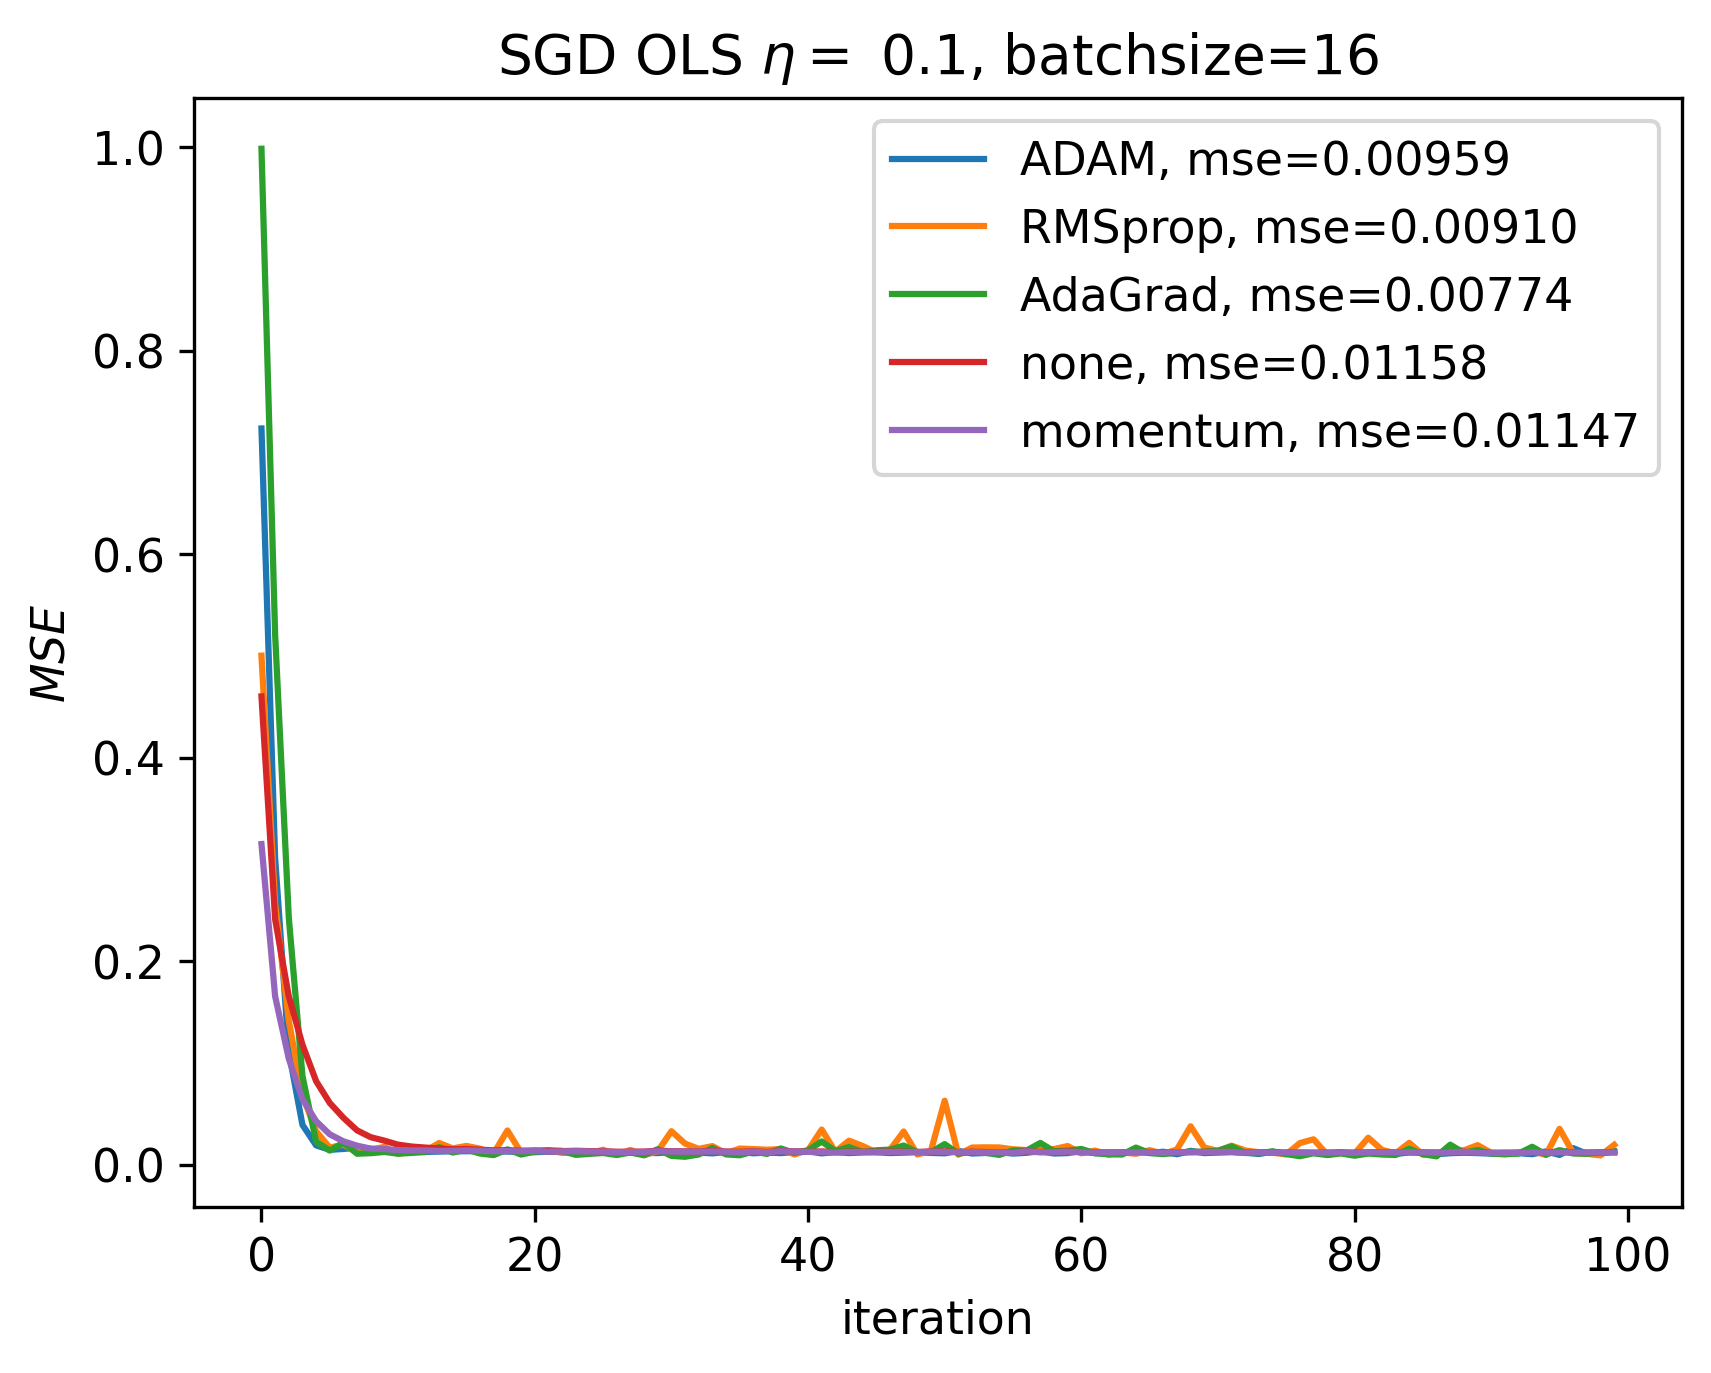
\includegraphics[width=\textwidth]{../figures/SGD_methods_OLS_eta_0.1.png}
        \caption{SGD}
        \label{fig:}
    \end{subfigure}
    \begin{subfigure}{.5\textwidth}
        \centering
        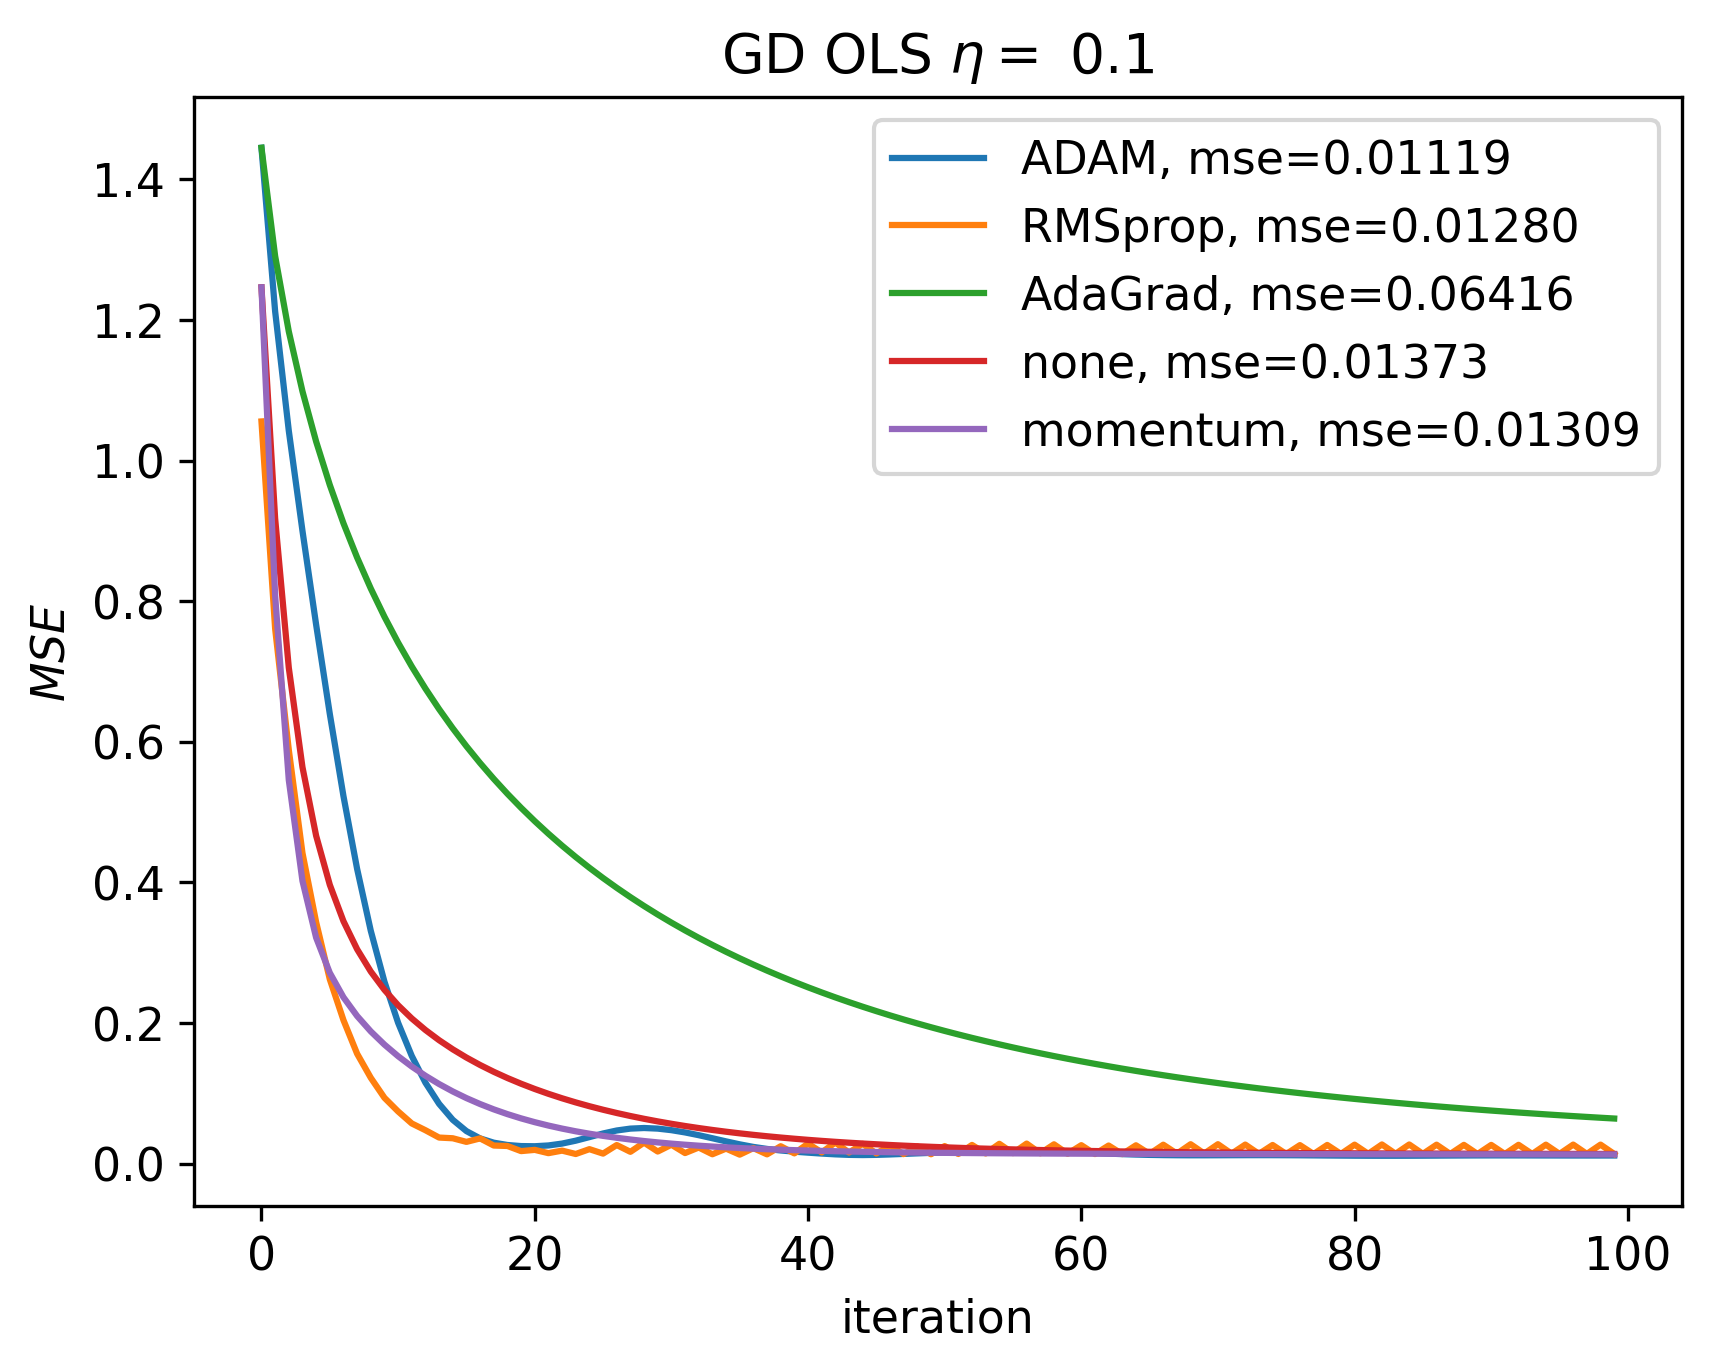
\includegraphics[width=\textwidth]{../figures/GD_methods_OLS_eta_0.1.png}
        \caption{GD}
        \label{fig:}
    \end{subfigure}
    \caption{$MSE$ for different tuning methods for both SGD and GD using $n=100$ data points with a 80-20 train-test split from a 4th order polynomial, a learning rate of $\eta=0.1$ and for SGD a batch size of 16 giving 5 mini batches. $MSE$ has been evaluated at each iteration using test data.}
    \label{fig:compare_GD_SGD}
\end{figure}
We see that SGD needs fewer iterations than GD in order to perform well. We also see a difference in how well the different tuning methods perform, and how fast they converge towards a low $MSE$.

When looking at the same methods for a lower learning rate of $\eta=0.01$ we get the following plots in figure \ref{fig:compare_GD_SGD_2}
\begin{figure}[H]
    \begin{subfigure}{.5\textwidth}
        \centering
        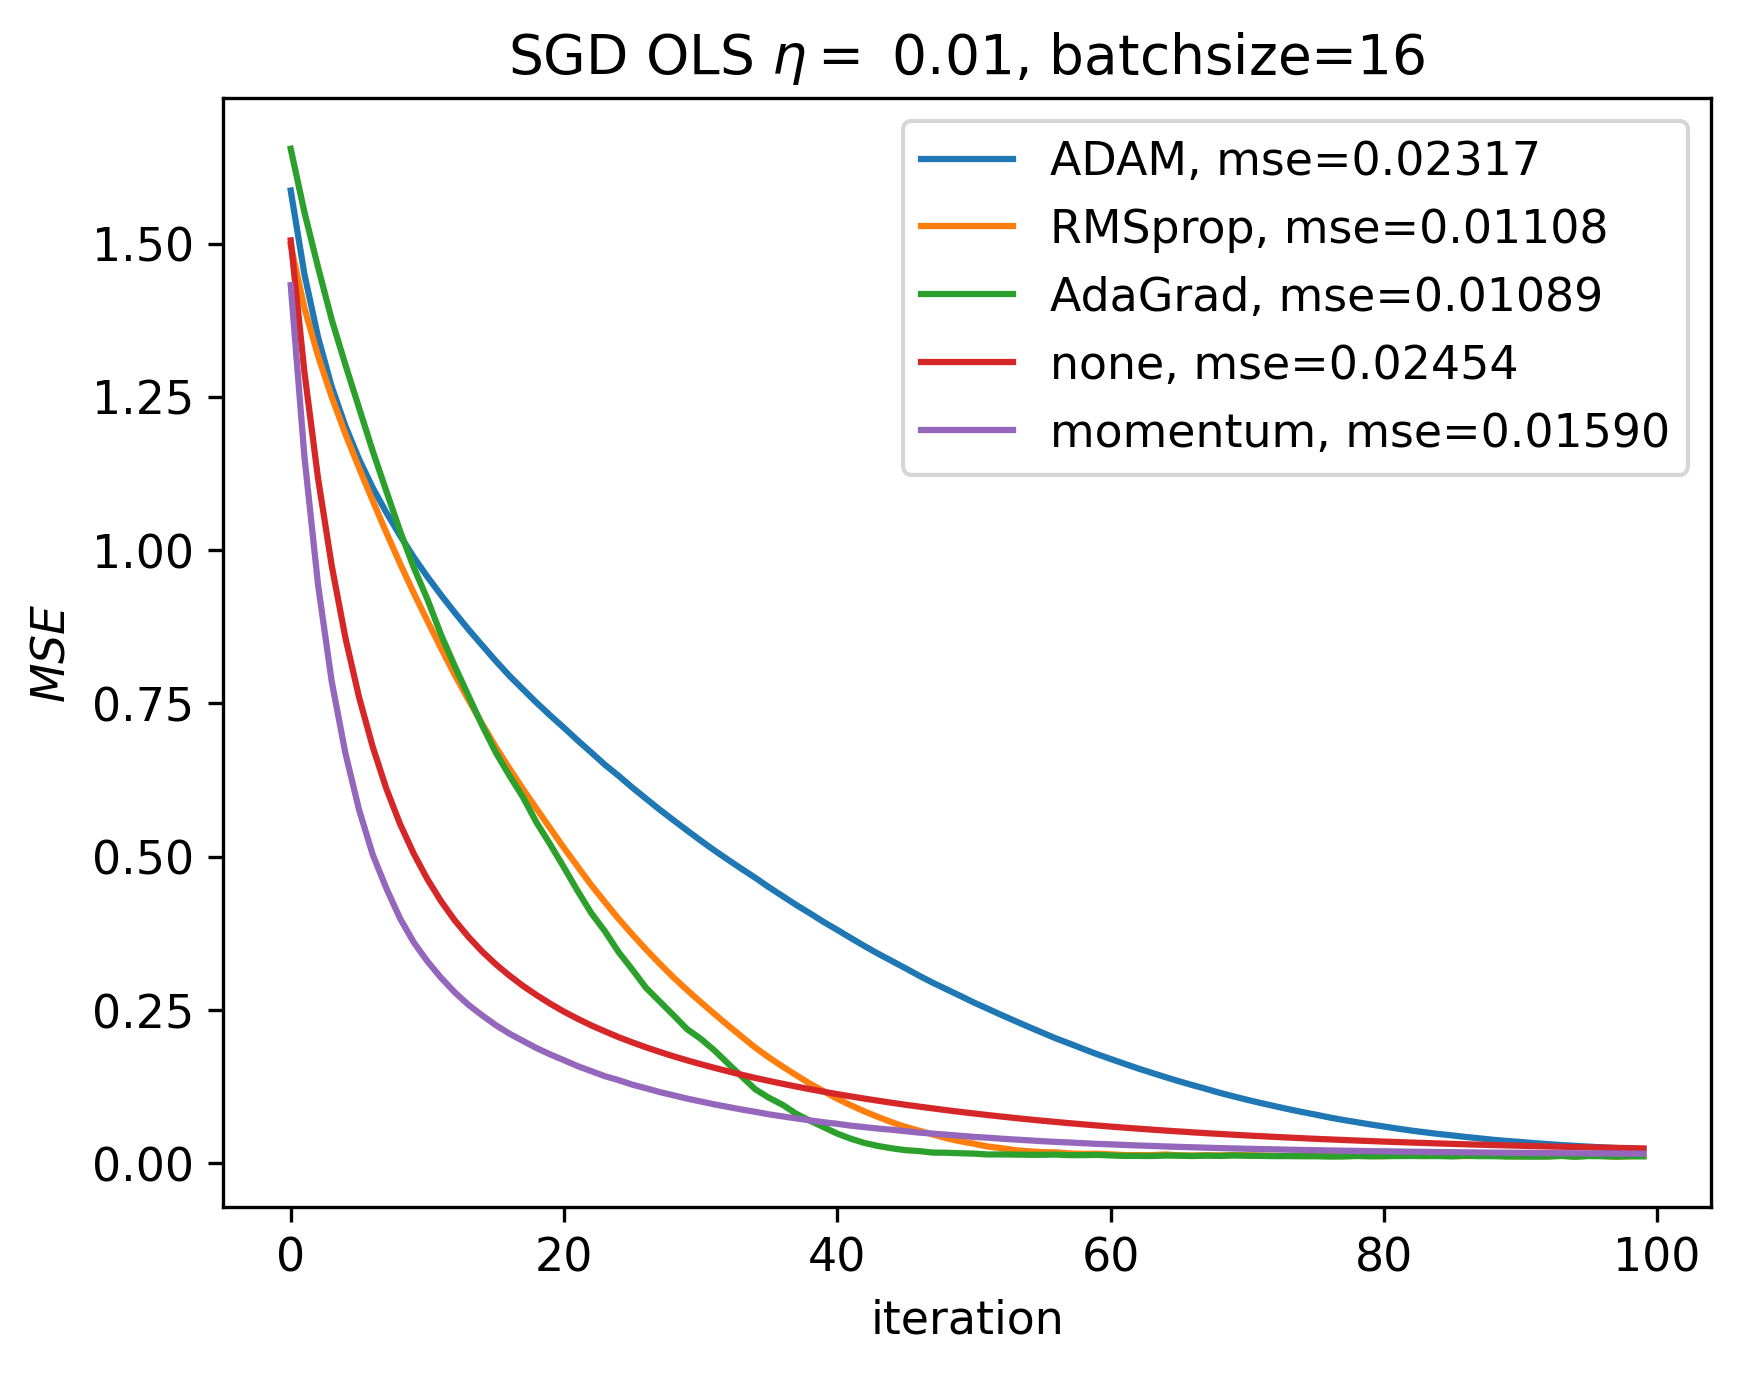
\includegraphics[width=\textwidth]{../figures/SGD_methods_OLS_eta_0.01.png}
        \caption{SGD}
        \label{fig:}
    \end{subfigure}
    \begin{subfigure}{.5\textwidth}
        \centering
        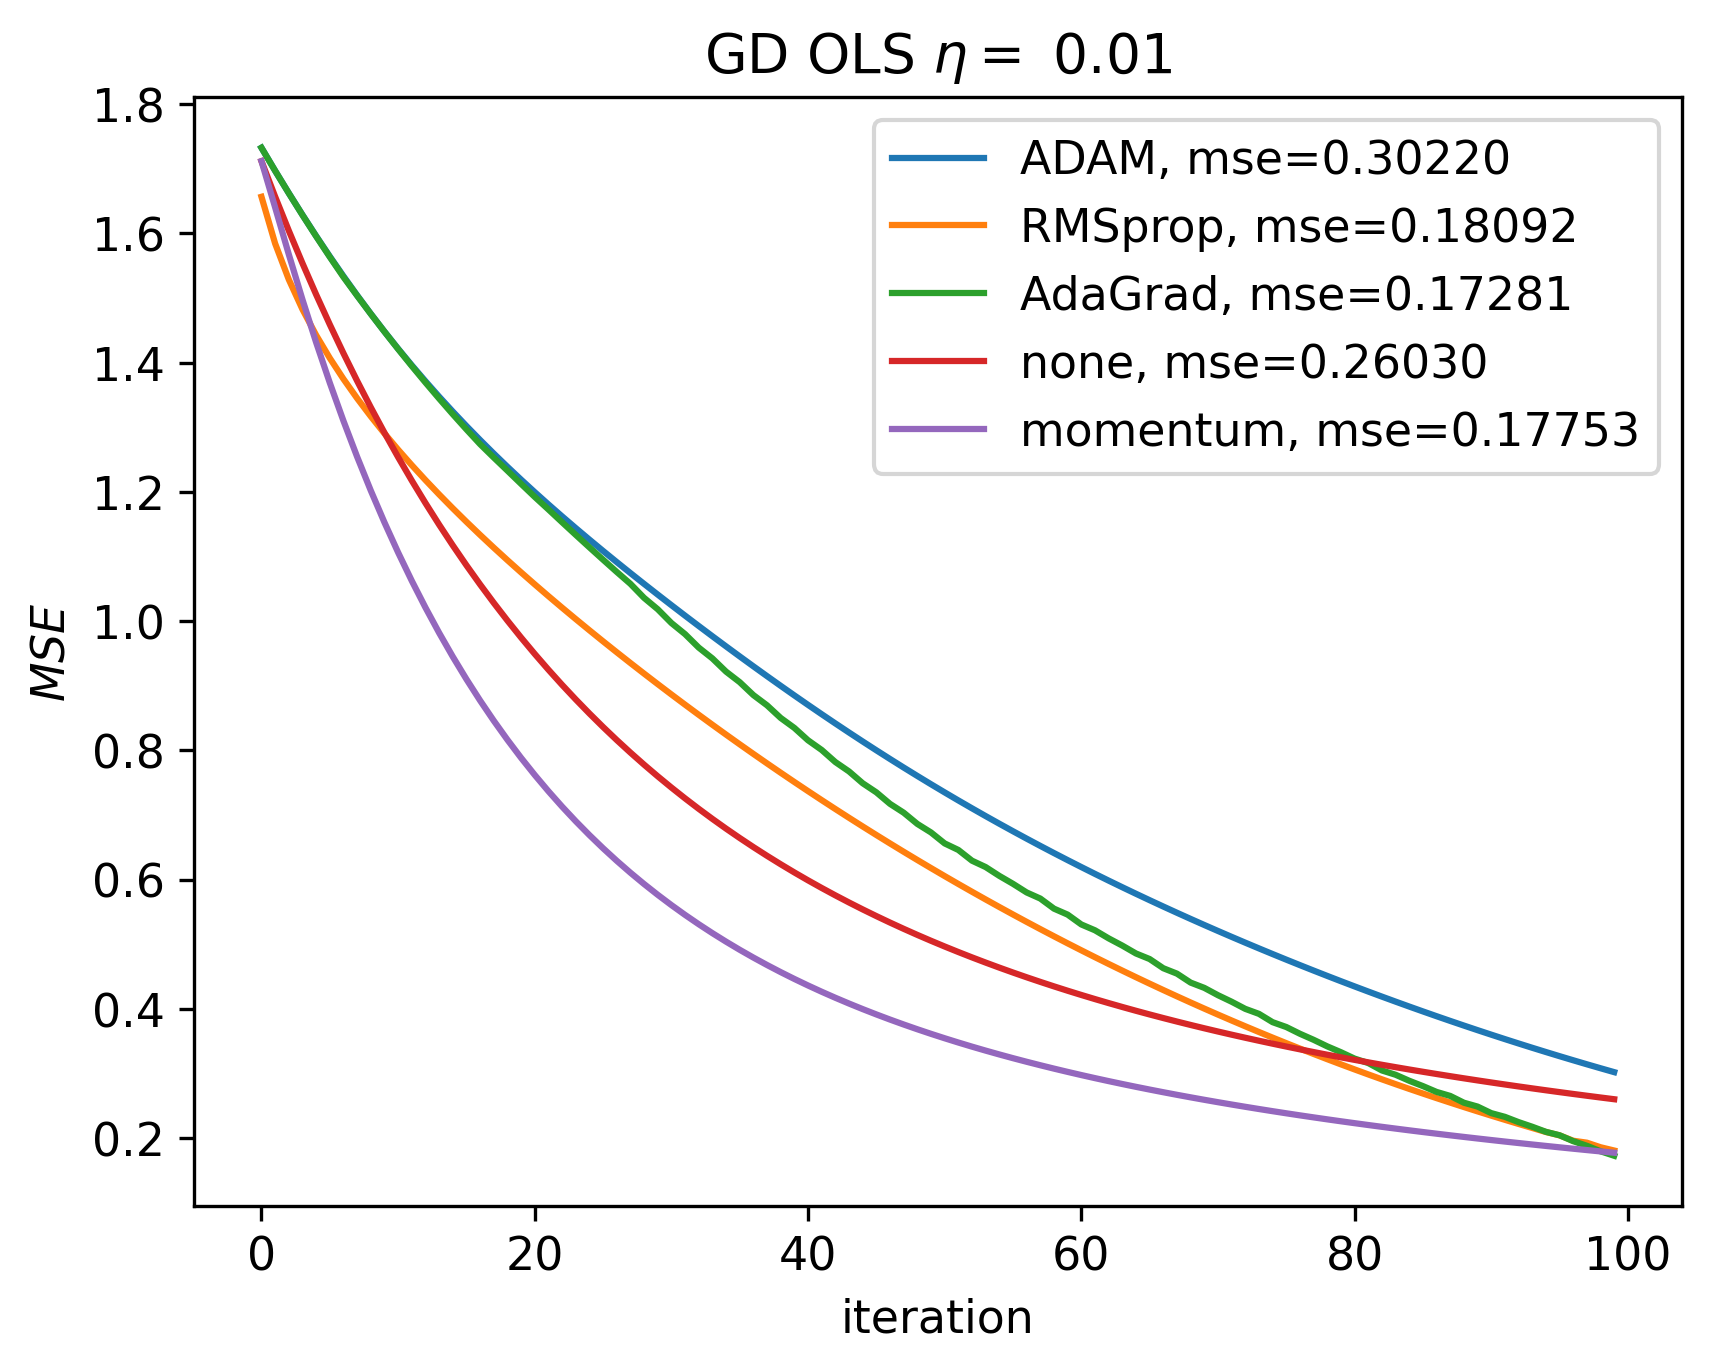
\includegraphics[width=\textwidth]{../figures/GD_methods_OLS_eta_0.01.png}
        \caption{GD}
        \label{fig:}
    \end{subfigure}
    \caption{$MSE$ for different tuning methods for both SGD and GD using $n=100$ data points with a 80-20 train-test split from a 4th order polynomial, a learning rate of $\eta=0.01$, and for SGD a batch size of 16 giving 5 mini batches. $MSE$ has been evaluated at each iteration using the training data.}
    \label{fig:compare_GD_SGD_2}
\end{figure}
In figure \ref{fig:compare_GD_SGD_2} we see the same as in figure \ref{fig:compare_GD_SGD} but now with an even slower convergence. We also see that the tuning methods for GD does not converge after 100 iterations, while SGD seem to start converging, giving $MSE$ values close to what we saw for a learning rate $\eta =0.1$ in figure \ref{fig:compare_GD_SGD}.

The minimum $MSE$ values for the different methods in figure \ref{fig:compare_GD_SGD} and \ref{fig:compare_GD_SGD_2} is shown in table \ref{tab:OLS_compare}
\begin{table}[H]
    \centering
    \caption{$MSE$ using test data for OLS and the different tuning methods for GD and SGD using  $\eta=0.01$ and $\eta=0.1$ over 100 iterations}
    \label{tab:OLS_compare}
    \begin{tabular}{|c|c|c|c|c|c|c|}
        \hline
        Method          & OLS     & AdaGrad & no tune & Momentum & RMSprop & ADAM    \\
        \hline
        SGD $\eta=0.1$  & 0.00980 & 0.00774 & 0.01158 & 0.01147  & 0.00910 & 0.00959 \\
        \hline
        GD  $\eta=0.1$  & 0.00980 & 0.06416 & 0.01373 & 0.01309  & 0.01280 & 0.01119 \\
        \hline
        SGD $\eta=0.01$ & 0.00980 & 0.01089 & 0.02454 & 0.01590  & 0.01108 & 0.02317 \\
        \hline
        GD  $\eta=0.01$ & 0.00980 & 1.26583 & 0.26030 & 0.17753  & 0.18092 & 0.30220 \\
        \hline
    \end{tabular}
\end{table}
In table \ref{tab:OLS_compare} above we see that the overall best performer is SGD with AdaGrad as tuning function reaching the lowest $MSE$ of 0.00774 which together with RMSprop and ADAM is better than the OLS $MSE$. We also see that $SGD$ performs the best, and that AdaGrad, RMSprop and ADAM are the tuning methods with generally best results.

An analysis of the $MSE$ for Ridge regression for different choices of $\lambda$ and $\eta$ can be seen in figure  \ref{fig:compare_ridge_2} and \ref{fig:compare_ridge}.

\begin{figure}[H]
    \begin{subfigure}{.5\textwidth}
        \centering
        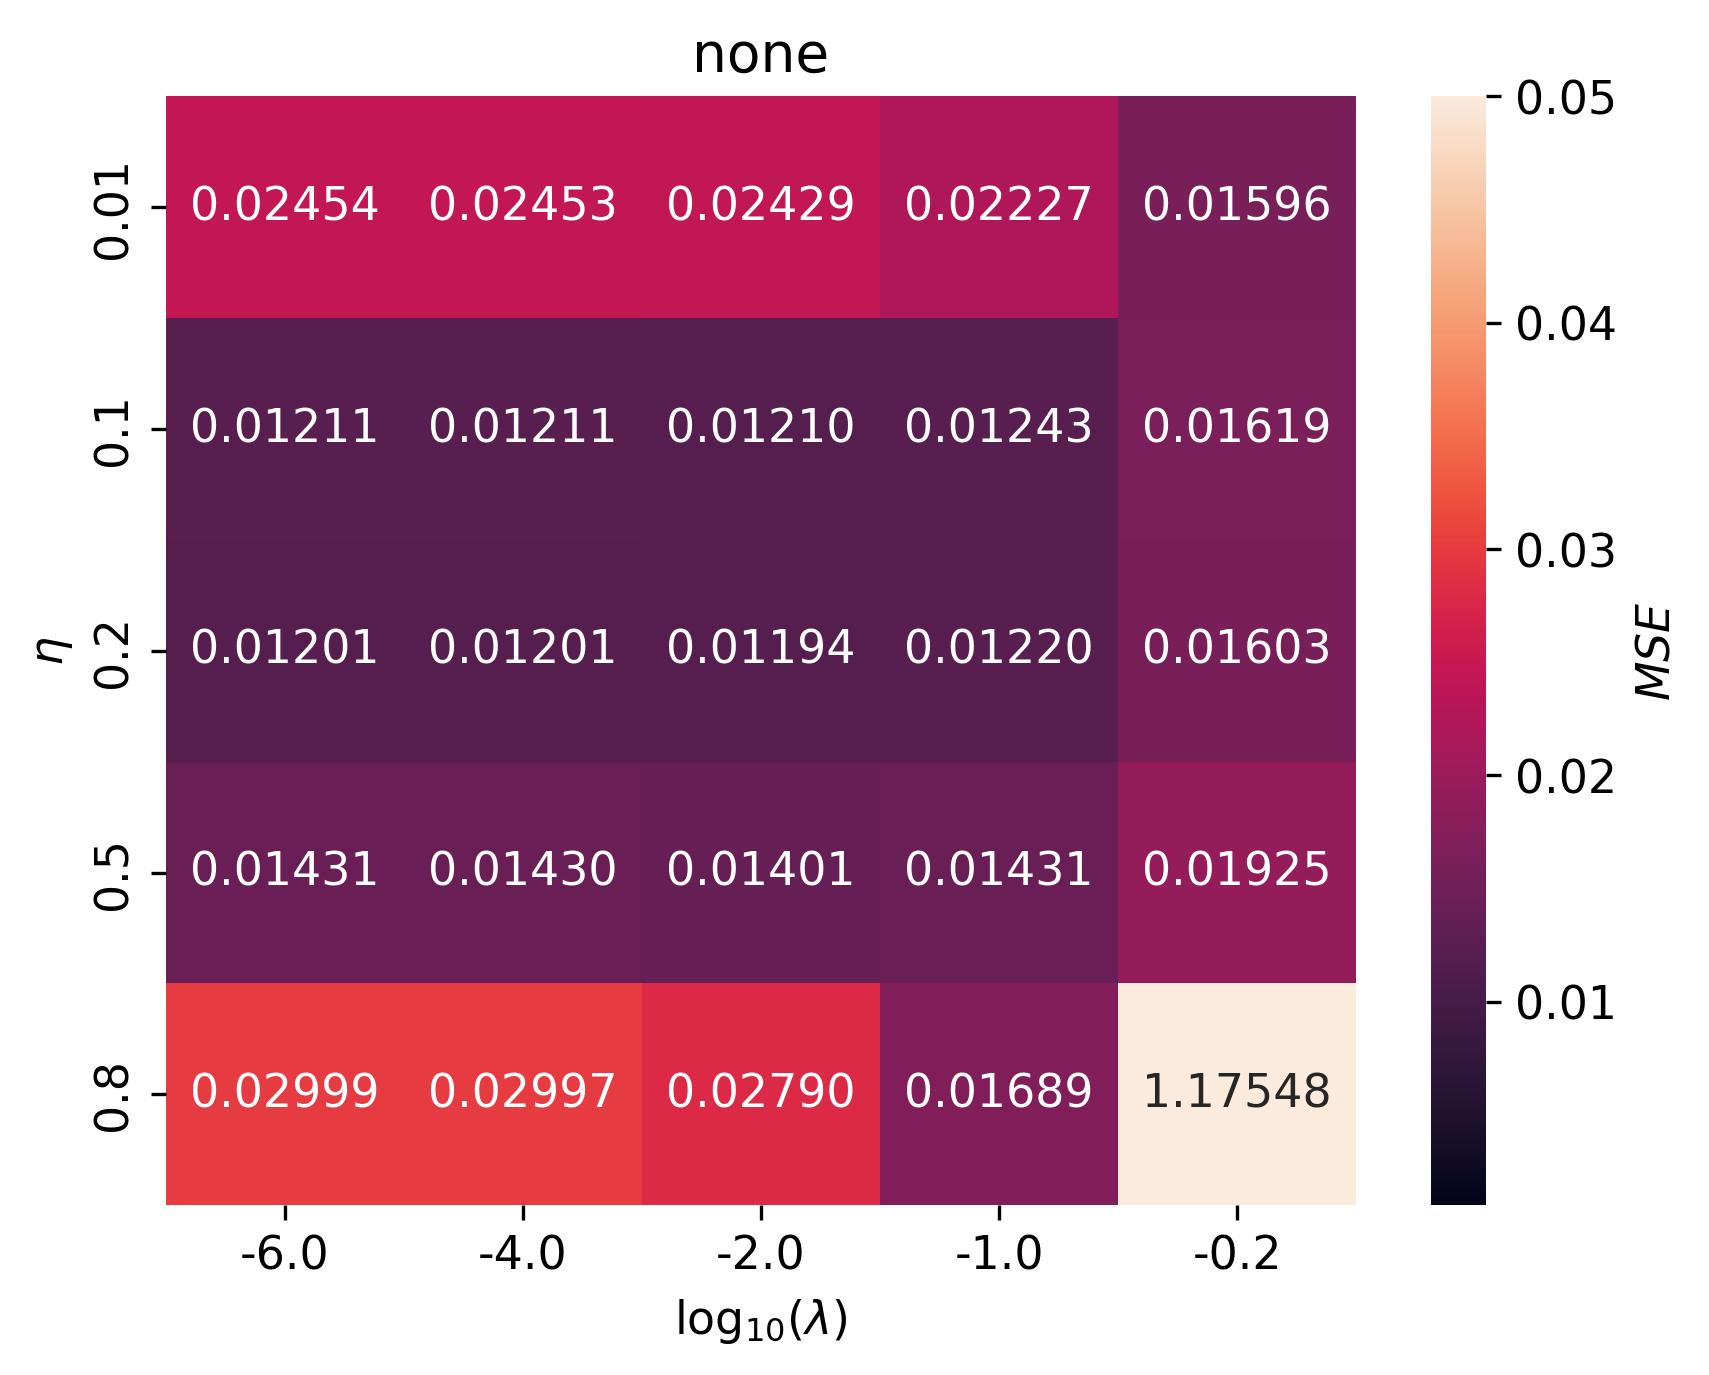
\includegraphics[width=\textwidth]{../figures/none_SGD_eta_lmb.png}
        \caption{SGD no tune}
        \label{fig:}
    \end{subfigure}
    \begin{subfigure}{.5\textwidth}
        \centering
        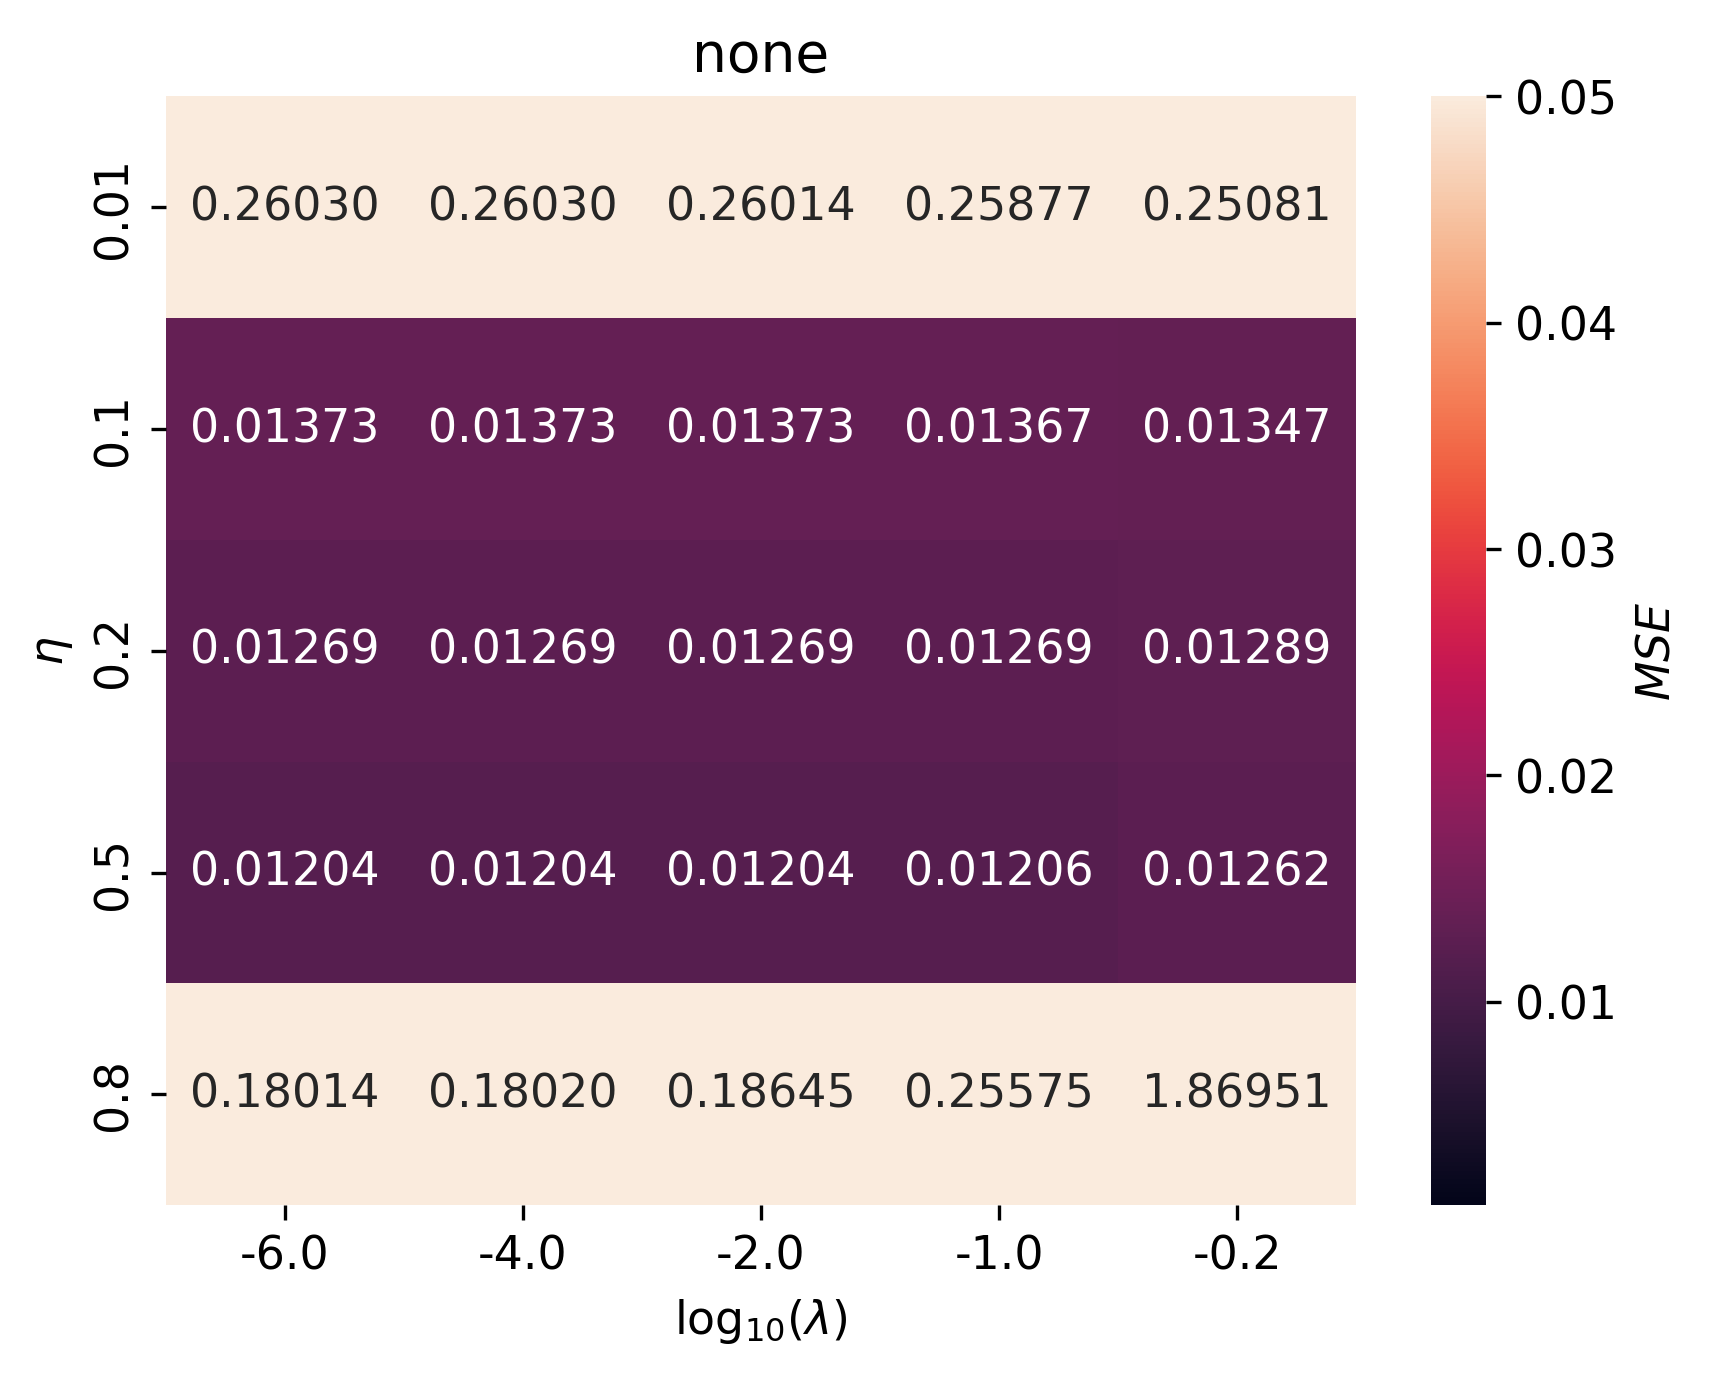
\includegraphics[width=\textwidth]{../figures/none_GD_eta_lmb.png}
        \caption{GD no tune}
        \label{fig:}
    \end{subfigure}
    \begin{subfigure}{.5\textwidth}
        \centering
        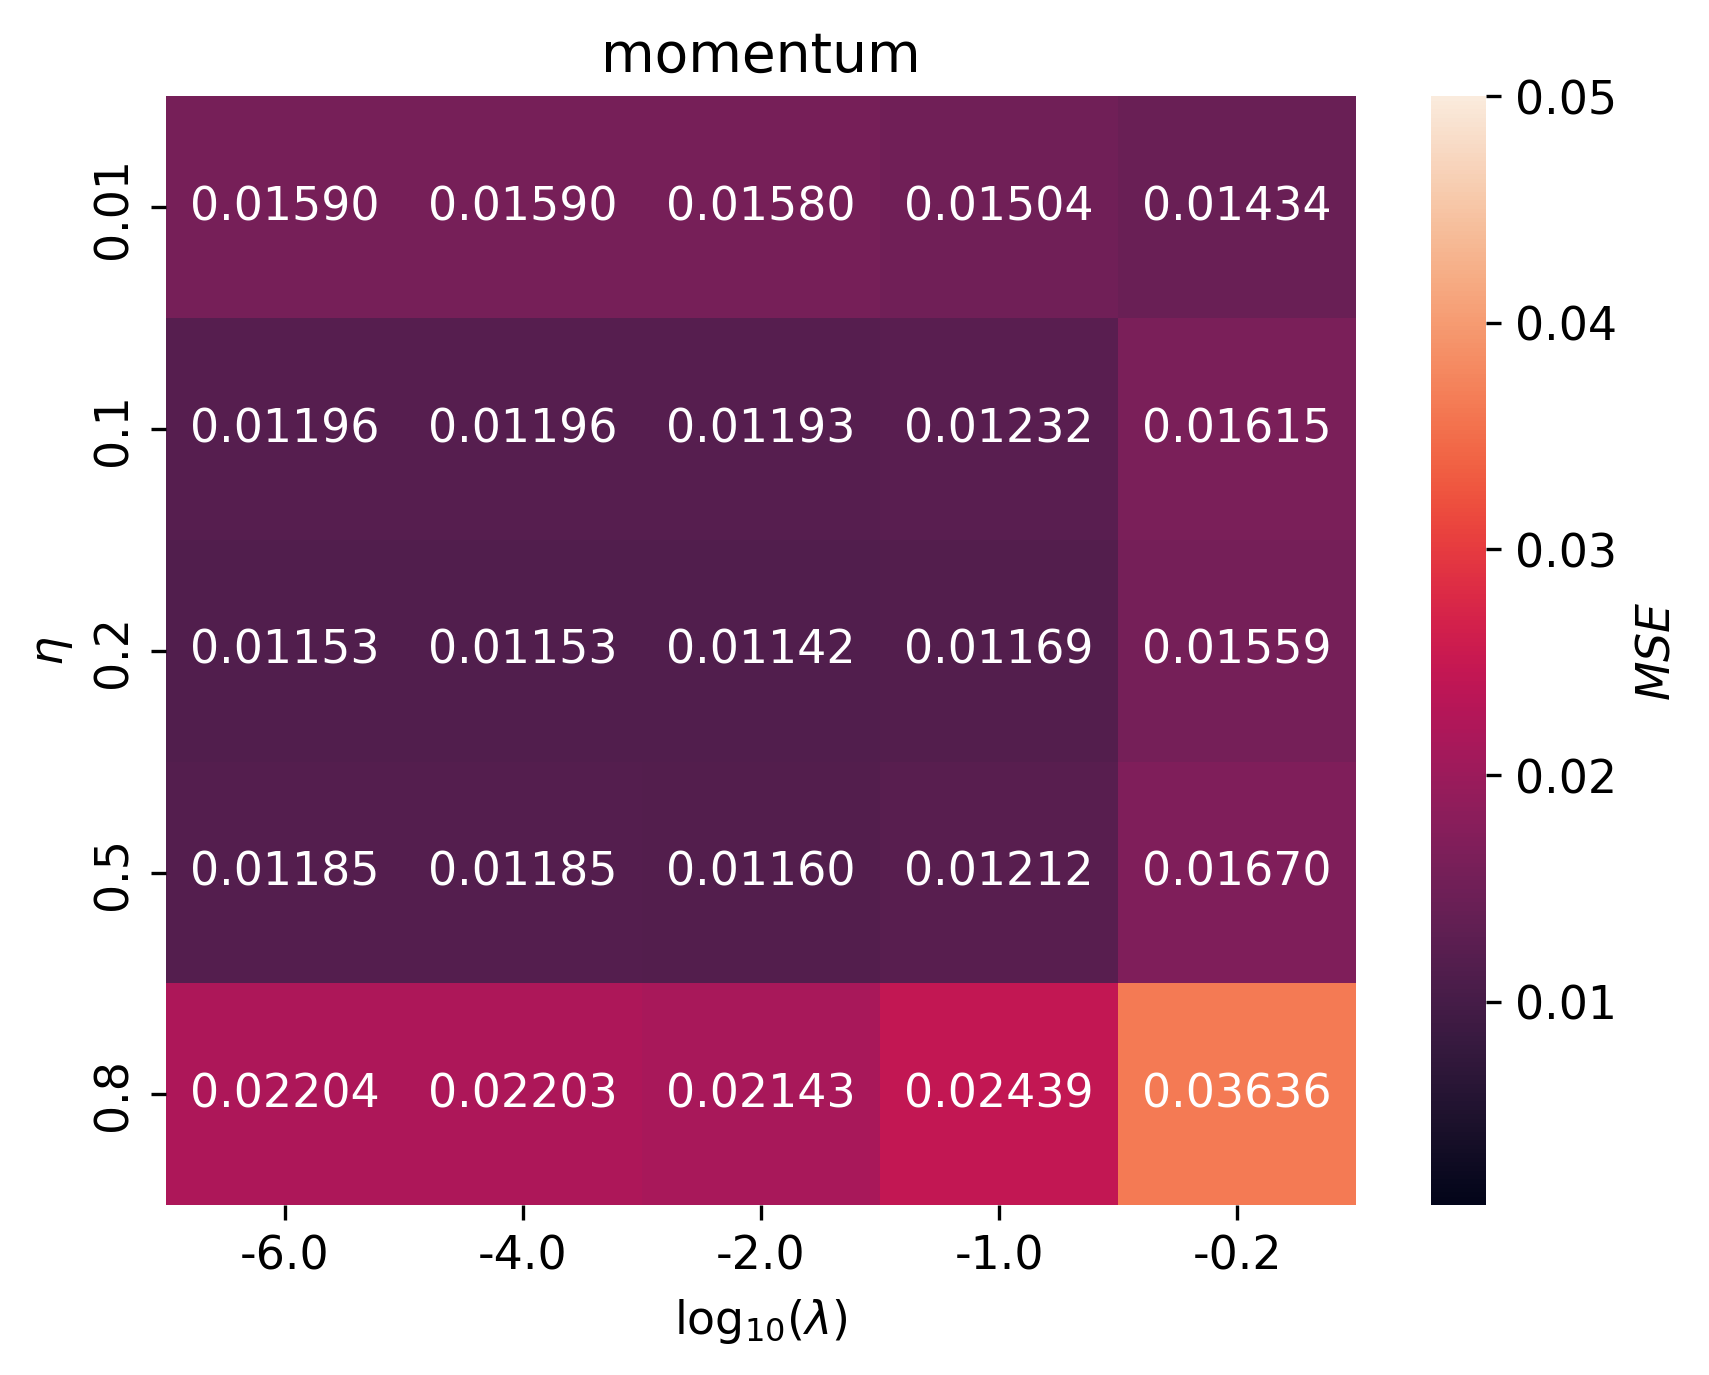
\includegraphics[width=\textwidth]{../figures/momentum_SGD_eta_lmb.png}
        \caption{SGD momentum}
        \label{fig:}
    \end{subfigure}
    \begin{subfigure}{.5\textwidth}
        \centering
        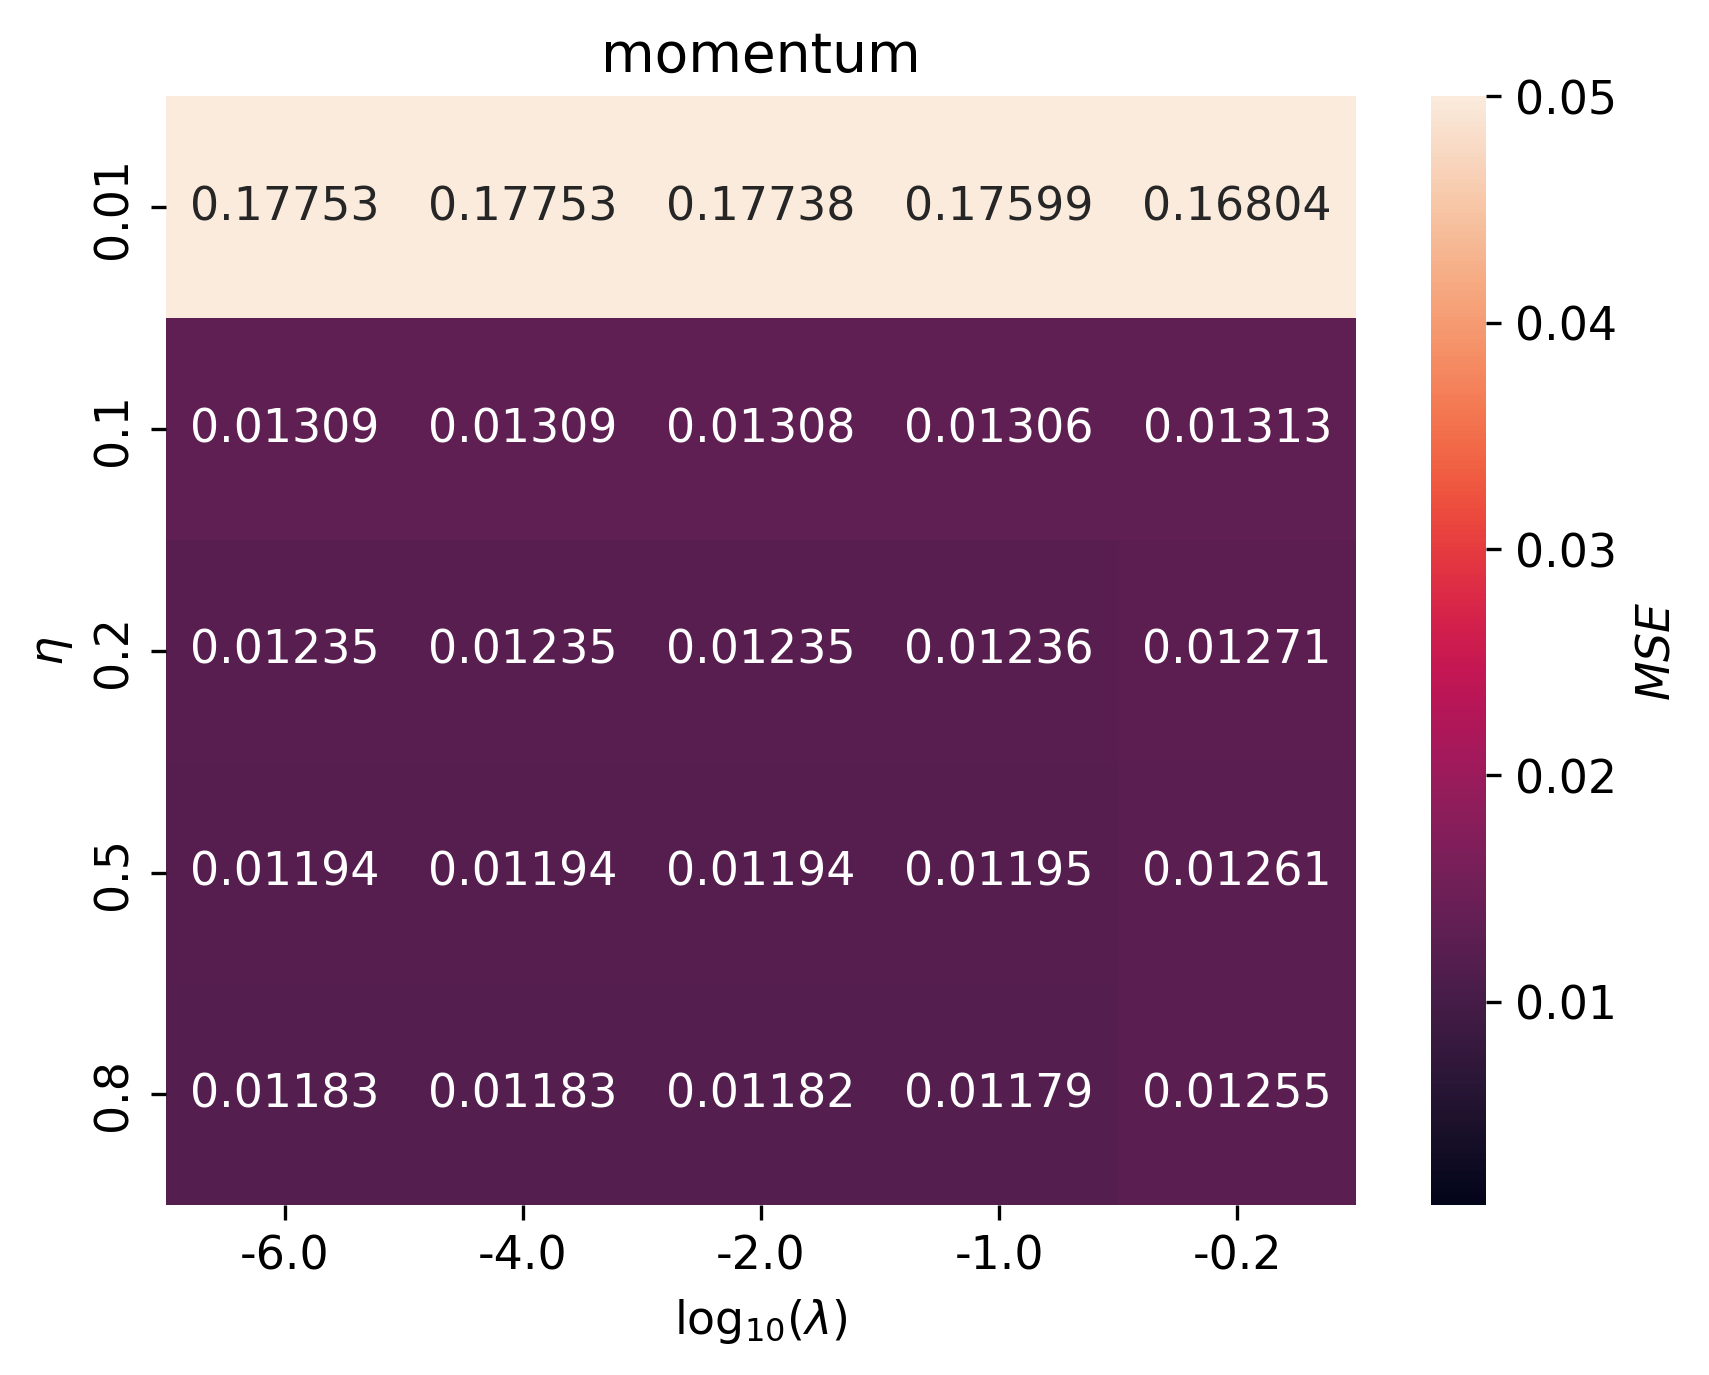
\includegraphics[width=\textwidth]{../figures/momentum_GD_eta_lmb.png}
        \caption{GD momentum}
        \label{fig:}
    \end{subfigure}
    \begin{subfigure}{.5\textwidth}
        \centering
        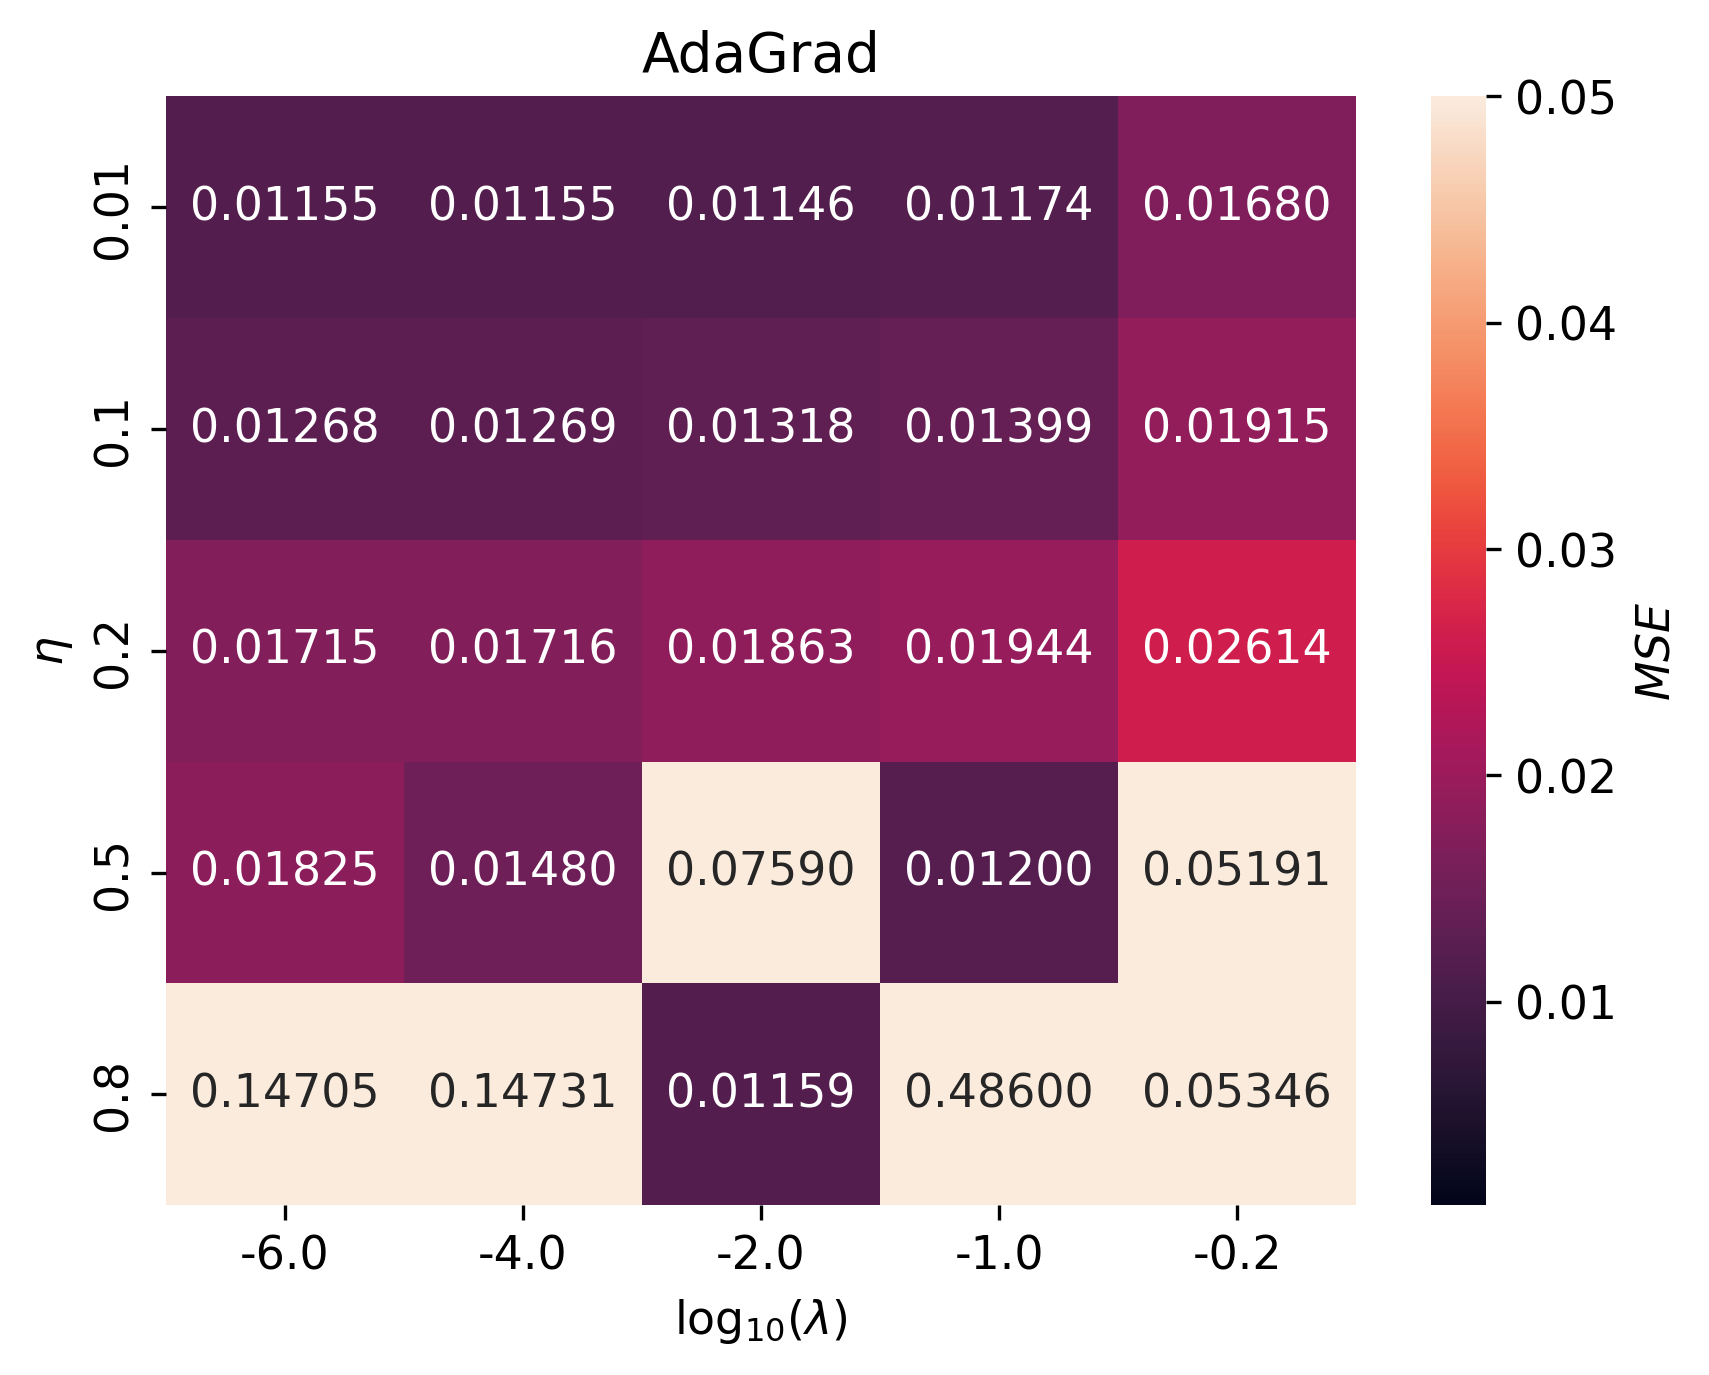
\includegraphics[width=\textwidth]{../figures/AdaGrad_SGD_eta_lmb.png}
        \caption{SGD AdaGrad}
        \label{fig:}
    \end{subfigure}
    \begin{subfigure}{.5\textwidth}
        \centering
        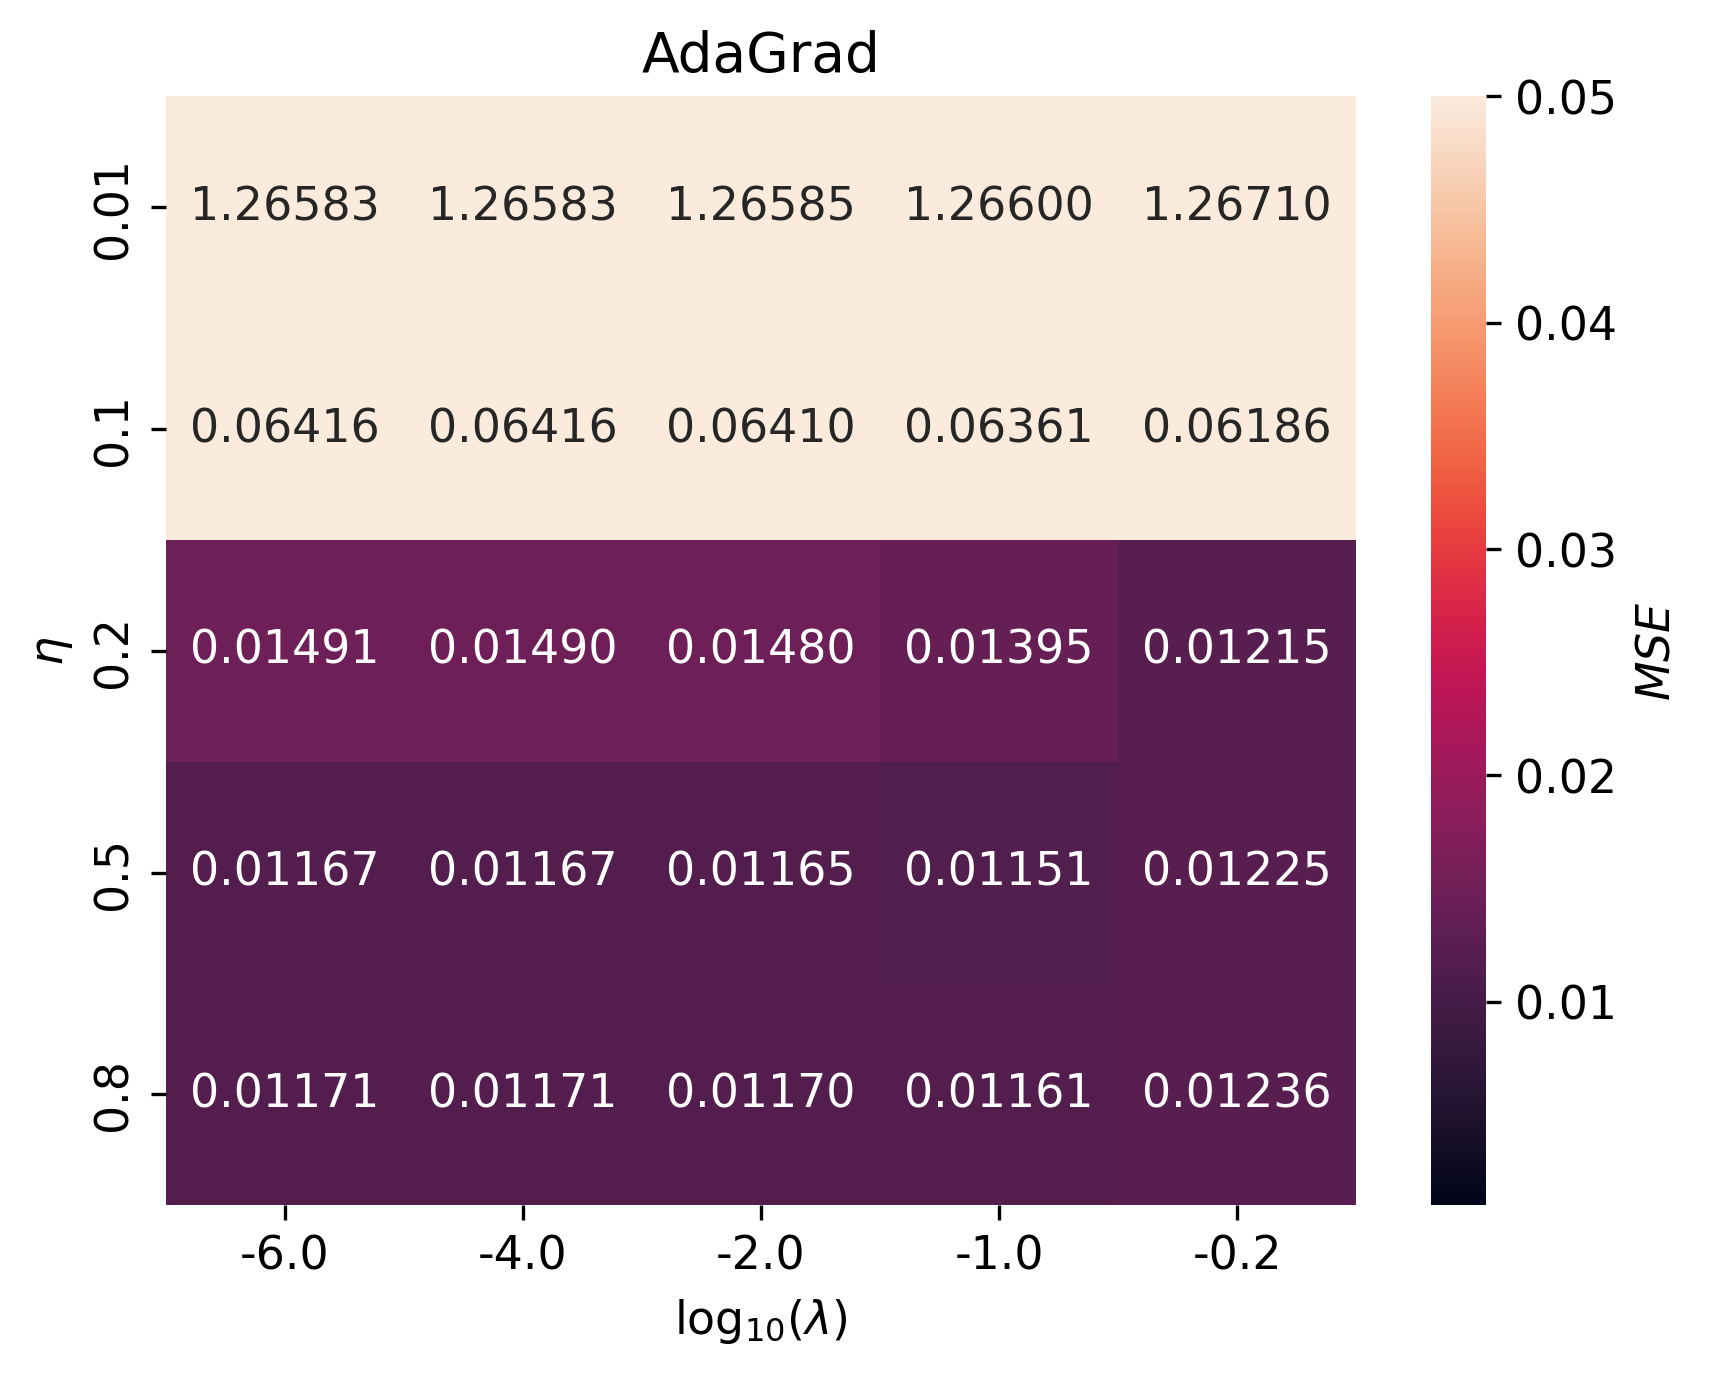
\includegraphics[width=\textwidth]{../figures/AdaGrad_GD_eta_lmb.png}
        \caption{GD AdaGrad}
        \label{fig:}
    \end{subfigure}
    \caption{$MSE$ for different methods for different choices of $\eta$ and $\lambda$ for both SGD (figures on the left) and GD (figures on the right) using $n=100$ data points from a 4th order polynomial with a batch size of 16 for SGD giving 5 mini batches}
    \label{fig:compare_ridge_2}
\end{figure}
\begin{figure}[H]

    \begin{subfigure}{.5\textwidth}
        \centering
        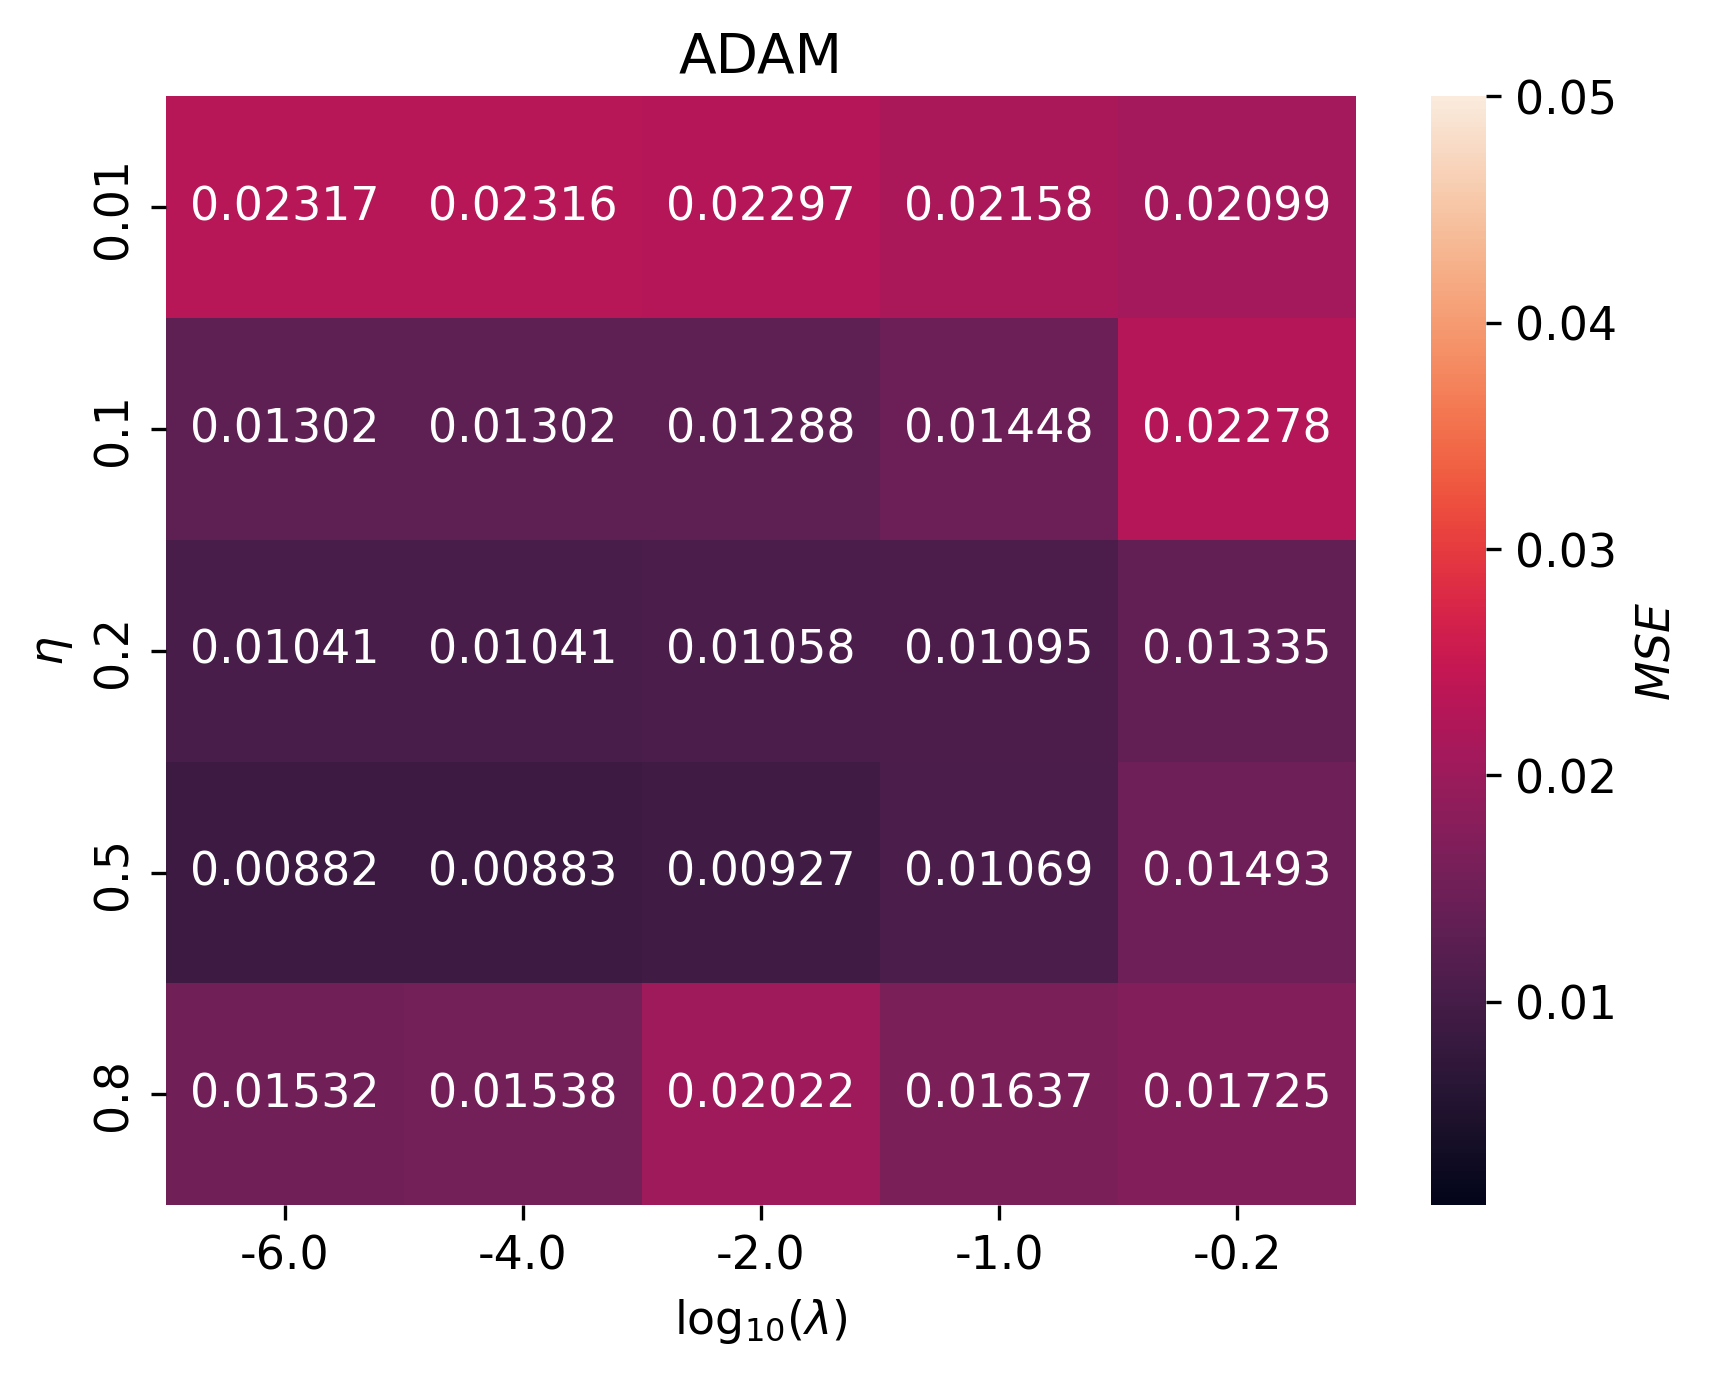
\includegraphics[width=\textwidth]{../figures/ADAM_SGD_eta_lmb.png}
        \caption{SGD ADAM}
        \label{fig:}
    \end{subfigure}
    \begin{subfigure}{.5\textwidth}
        \centering
        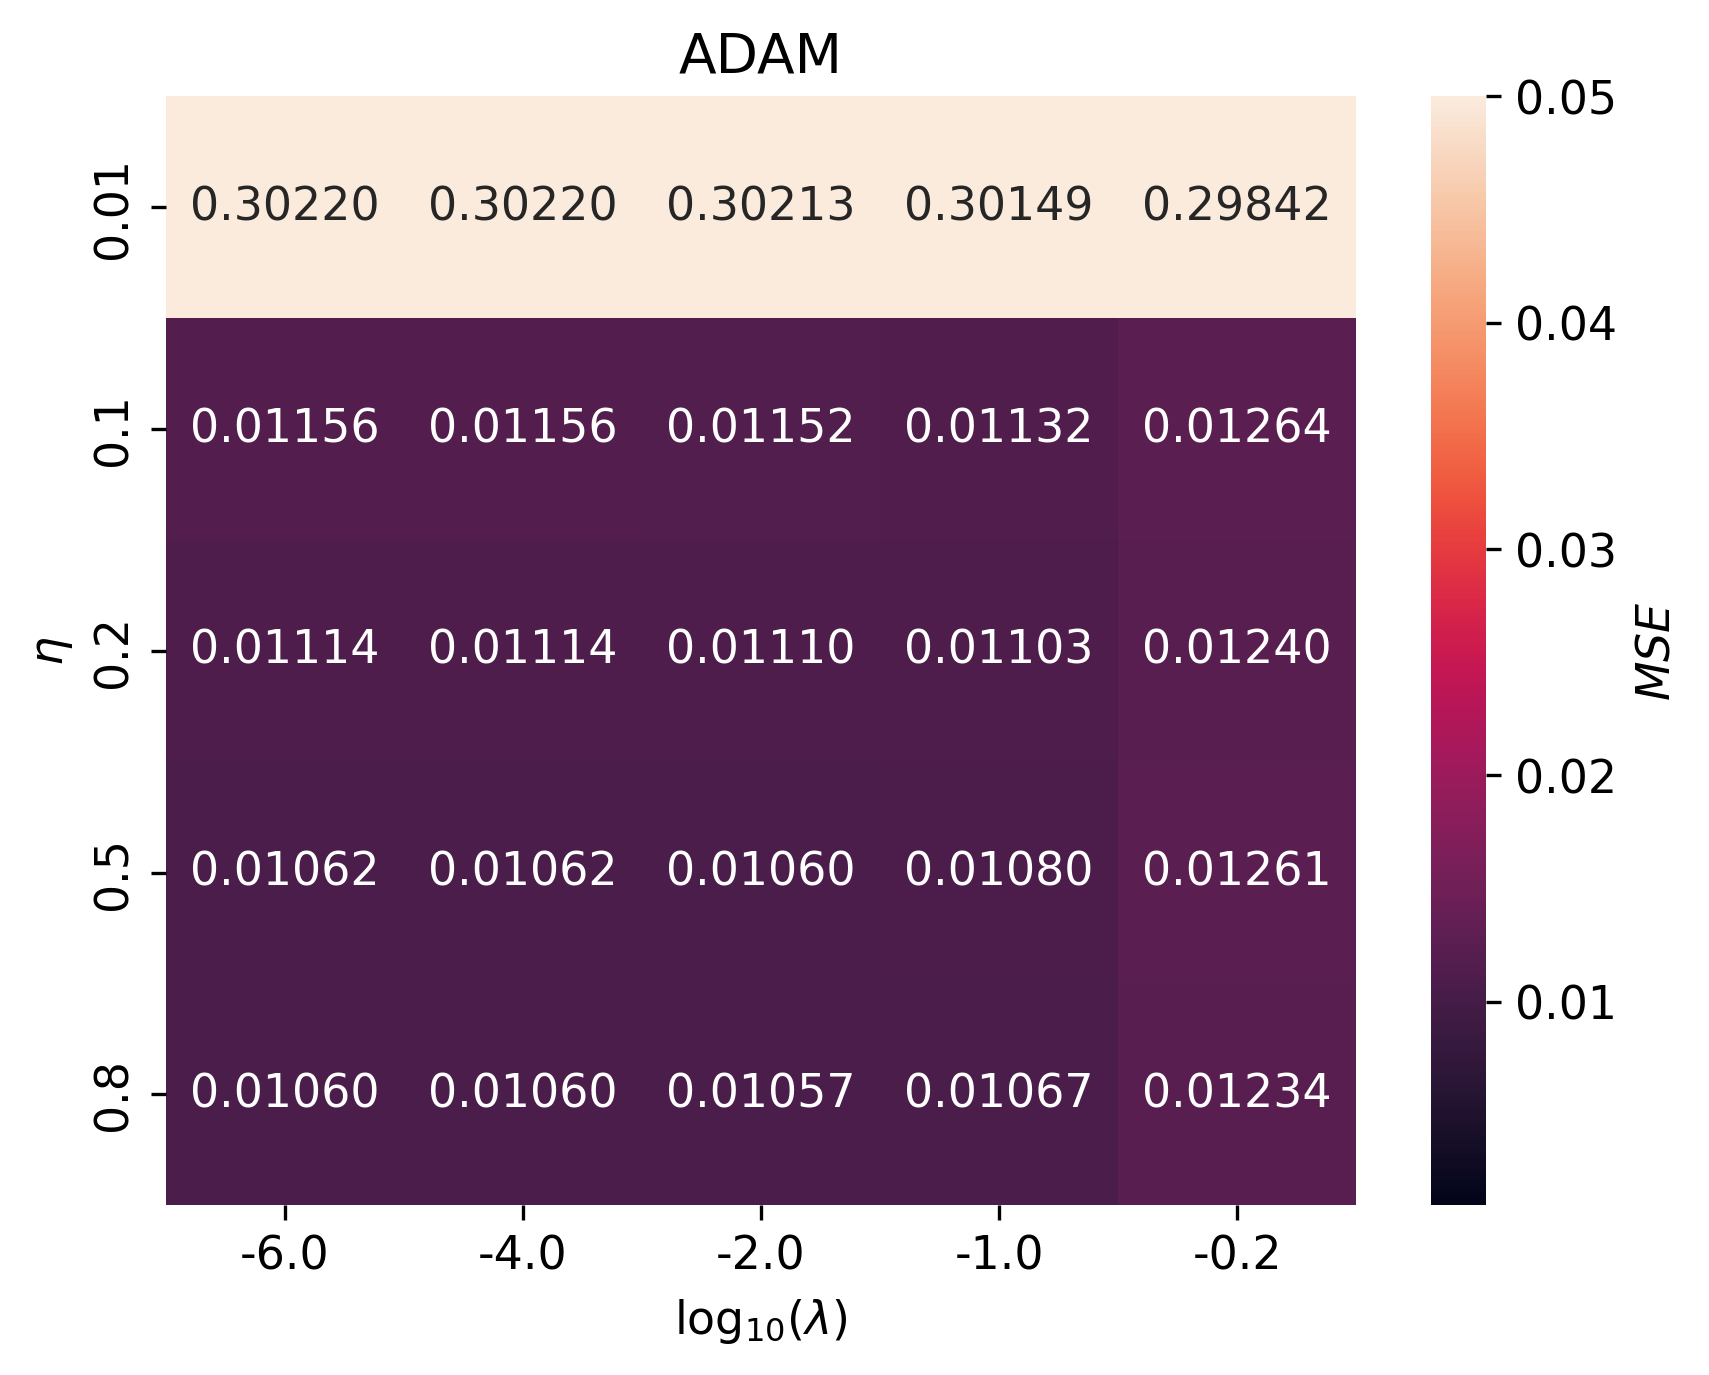
\includegraphics[width=\textwidth]{../figures/ADAM_GD_eta_lmb.png}
        \caption{GD ADAM}
        \label{fig:}
    \end{subfigure}
    \begin{subfigure}{.5\textwidth}
        \centering
        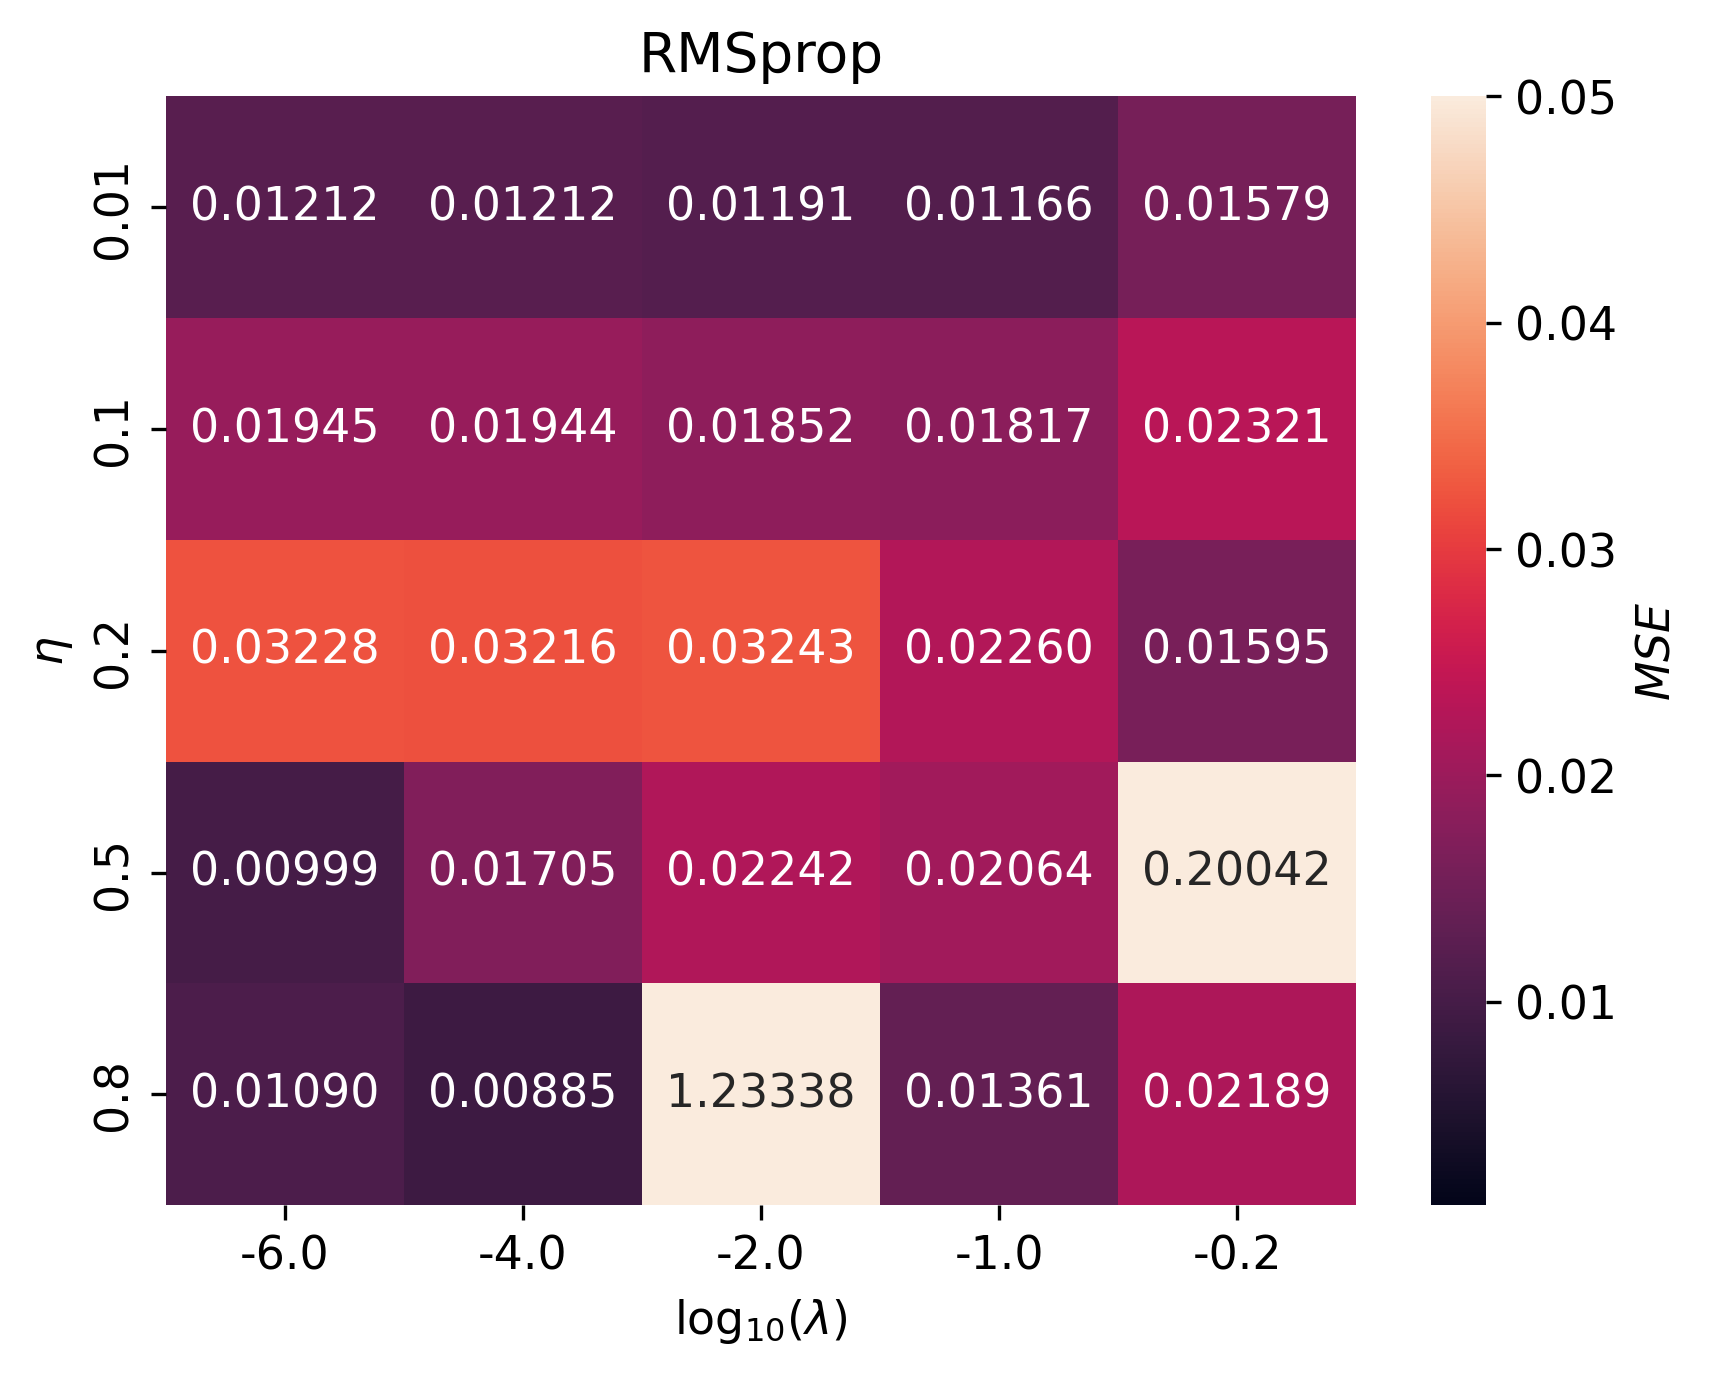
\includegraphics[width=\textwidth]{../figures/RMSprop_SGD_eta_lmb.png}
        \caption{SGD RMSprop}
        \label{fig:}
    \end{subfigure}
    \begin{subfigure}{.5\textwidth}
        \centering
        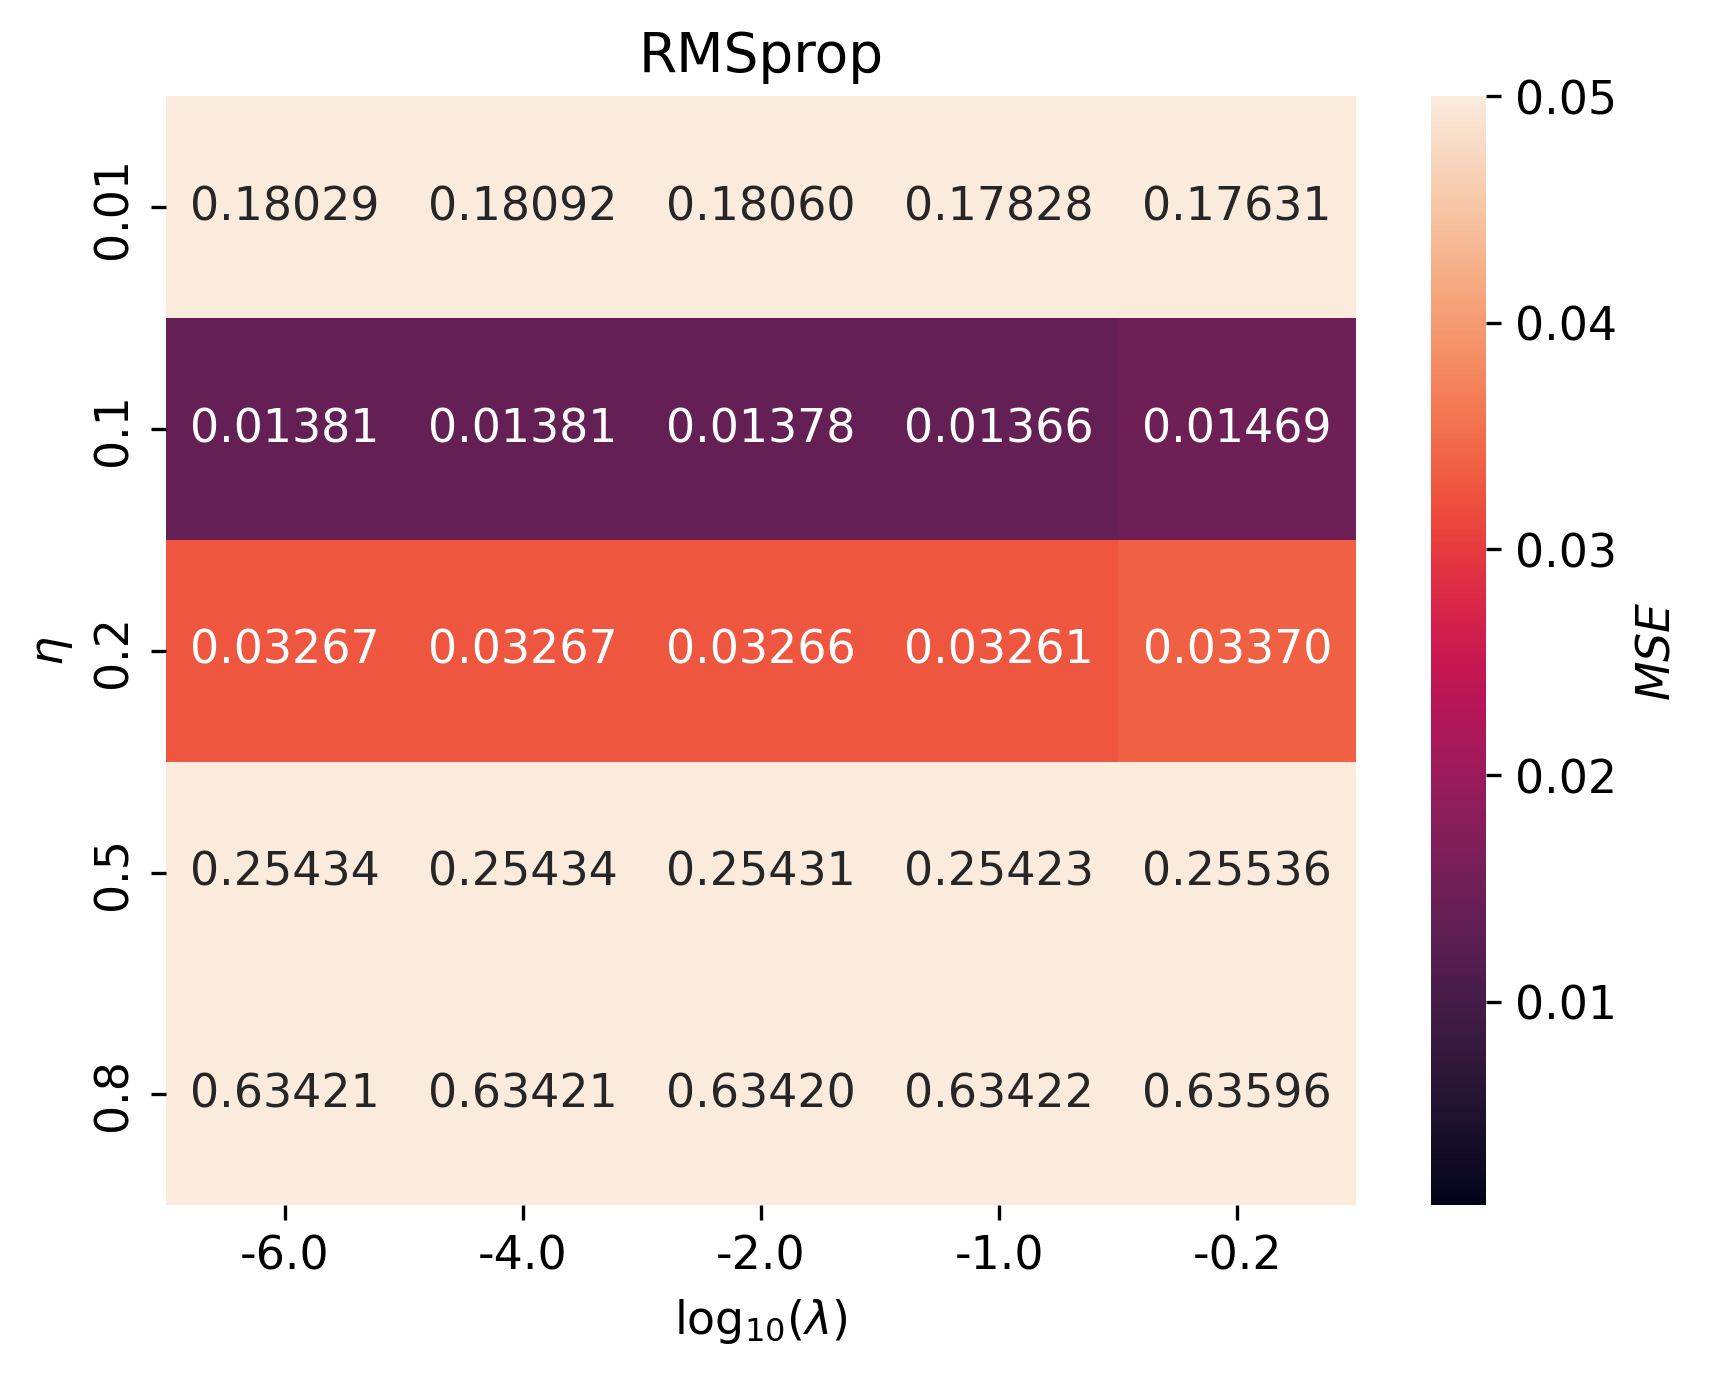
\includegraphics[width=\textwidth]{../figures/RMSprop_GD_eta_lmb.png}
        \caption{GD RMSprop}
        \label{fig:}
    \end{subfigure}
    \caption{$MSE$ for different methods for different choices of $\eta$ and $\lambda$ for both SGD (figures on the left) and GD (figures on the right) using $n=100$ data points from a 4th order polynomial with a batch size of 16 for SGD giving 5 mini batches}
    \label{fig:compare_ridge}
\end{figure}
In figure \ref{fig:compare_ridge} and \ref{fig:compare_ridge_2} we see that the methods vary in $MSE$ both when changing the learning rate $\eta$ and when changing the L2 norm $\lambda$. In table \ref{tab:ridge_compare_GD} and \ref{tab:ridge_compare_SGD} we see the lowest $MSE$ for each method together with the parameters used.
\begin{table}[H]
    \centering
    \caption{$MSE$ of ridge and the best performing tuning methods for SGD after 100 iterations}
    \label{tab:ridge_compare_SGD}
    \begin{tabular}{|c|c|c|c|c|c|c|}
        \hline
        Method    & ridge               & AdaGrad   & no tune   & Momentum  & RMSprop   & ADAM      \\
        \hline
        $MSE$     & 0.00980             & 0.01146   & 0.01194   & 0.01142   & 0.00885   & 0.00882   \\
        \hline
        $\lambda$ & $1.61\times10^{-7}$ & $10^{-2}$ & $10^{-2}$ & $10^{-2}$ & $10^{-4}$ & $10^{-6}$ \\
        \hline
        $\eta$    & -                   & 0.01      & 0.2       & 0.2       & 0.8       & 0.5       \\
        \hline
    \end{tabular}
\end{table}
\begin{table}[H]
    \centering
    \caption{$MSE$ of ridge and the best performing tuning methods for GD after 100 iterations}
    \label{tab:ridge_compare_GD}
    \begin{tabular}{|c|c|c|c|c|c|c|}
        \hline
        Method    & ridge               & AdaGrad   & no tune   & Momentum  & RMSprop   & ADAM      \\
        \hline
        $MSE$     & 0.00980             & 0.01151   & 0.01204   & 0.01179   & 0.01366   & 0.01057   \\
        \hline
        $\lambda$ & $1.61\times10^{-7}$ & $10^{-1}$ & $10^{-4}$ & $10^{-1}$ & $10^{-1}$ & $10^{-2}$ \\
        \hline
        $\eta$    & -                   & 0.5       & 0.5       & 0.8       & 0.1       & 0.8       \\
        \hline
    \end{tabular}
\end{table}

\begin{figure}[H]
    \begin{subfigure}{.5\textwidth}
        \centering
        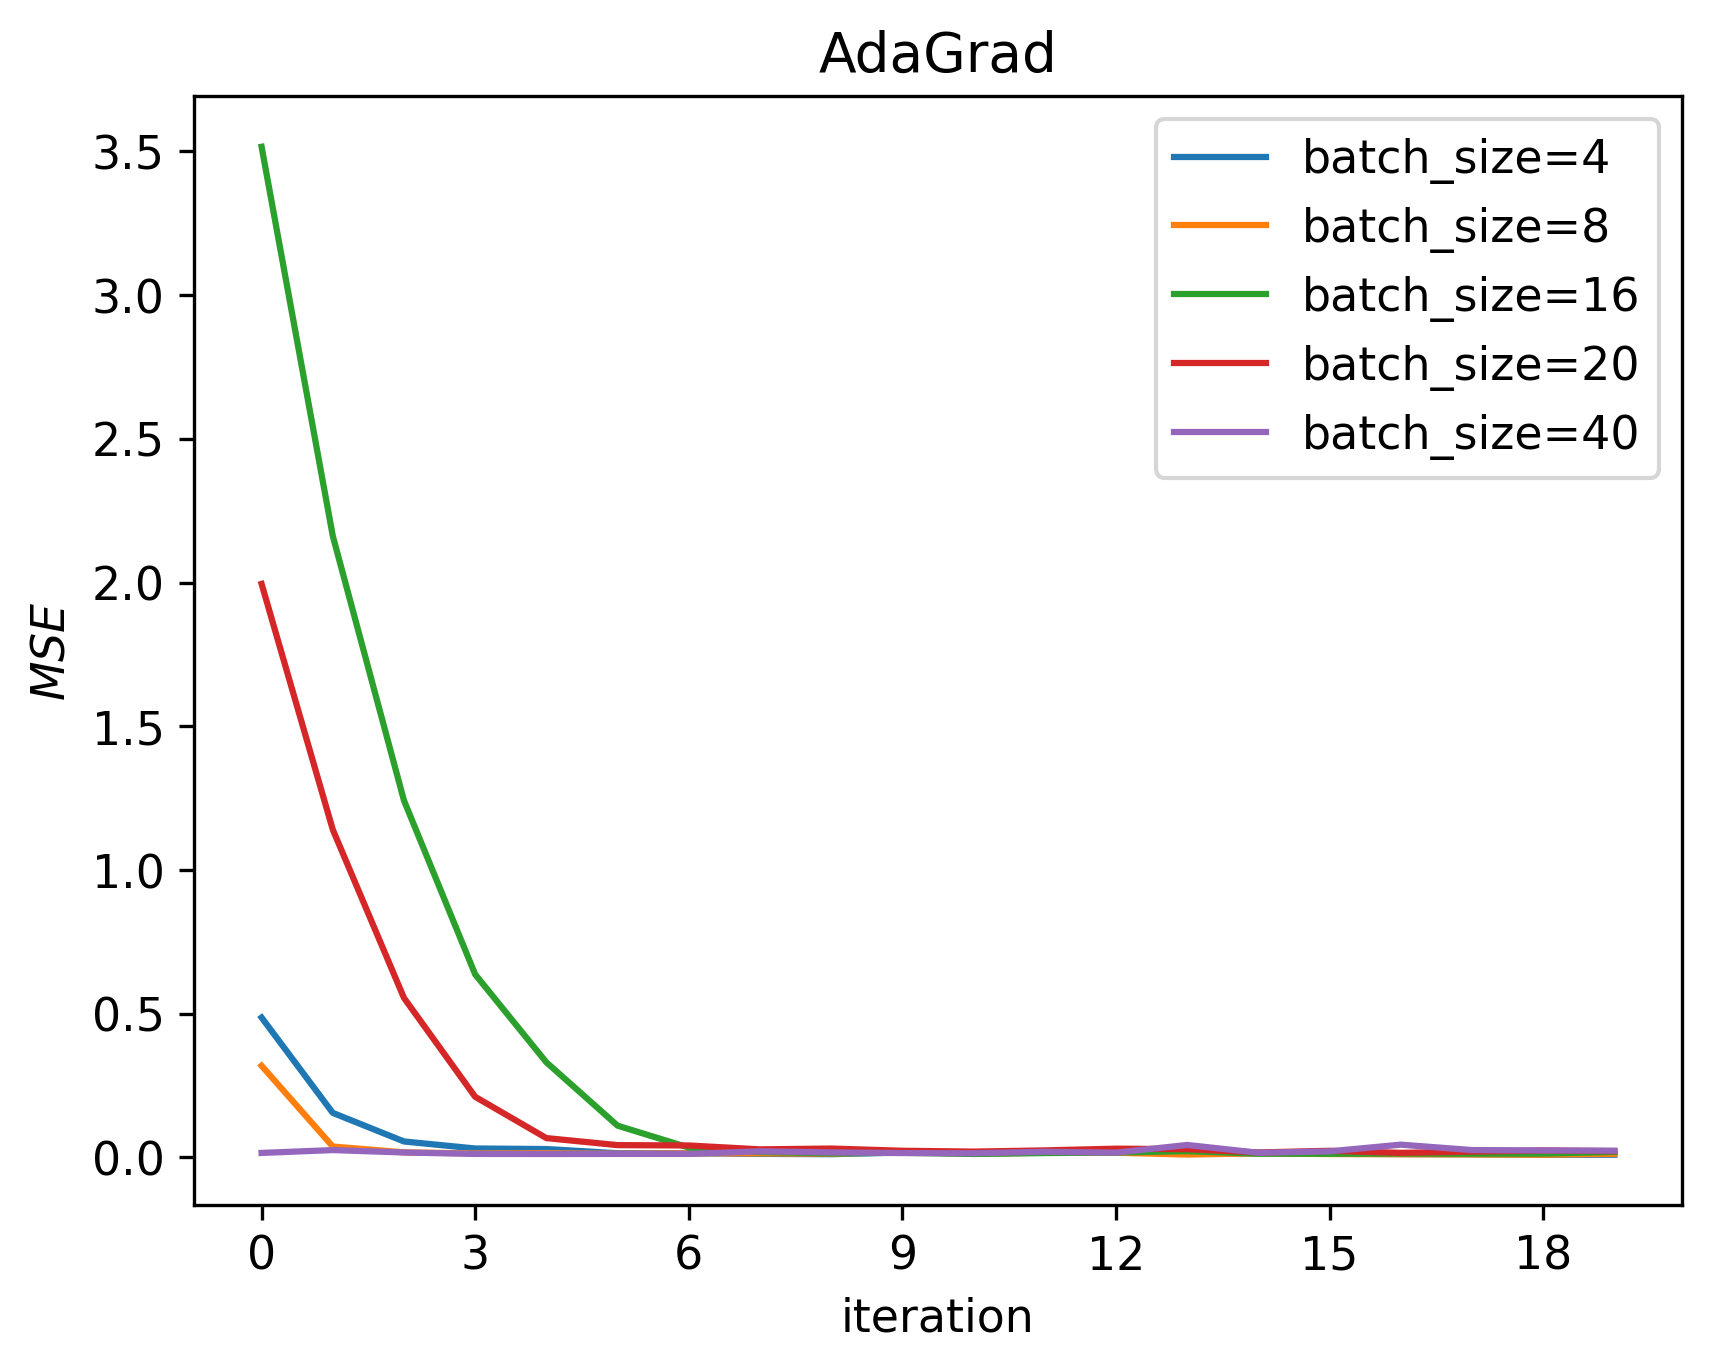
\includegraphics[width=.9\textwidth]{../figures/SGD_batch_size_AdaGrad.png}
        \caption{AdaGrad}
        \label{fig:}
    \end{subfigure}
    \begin{subfigure}{.5\textwidth}
        \centering
        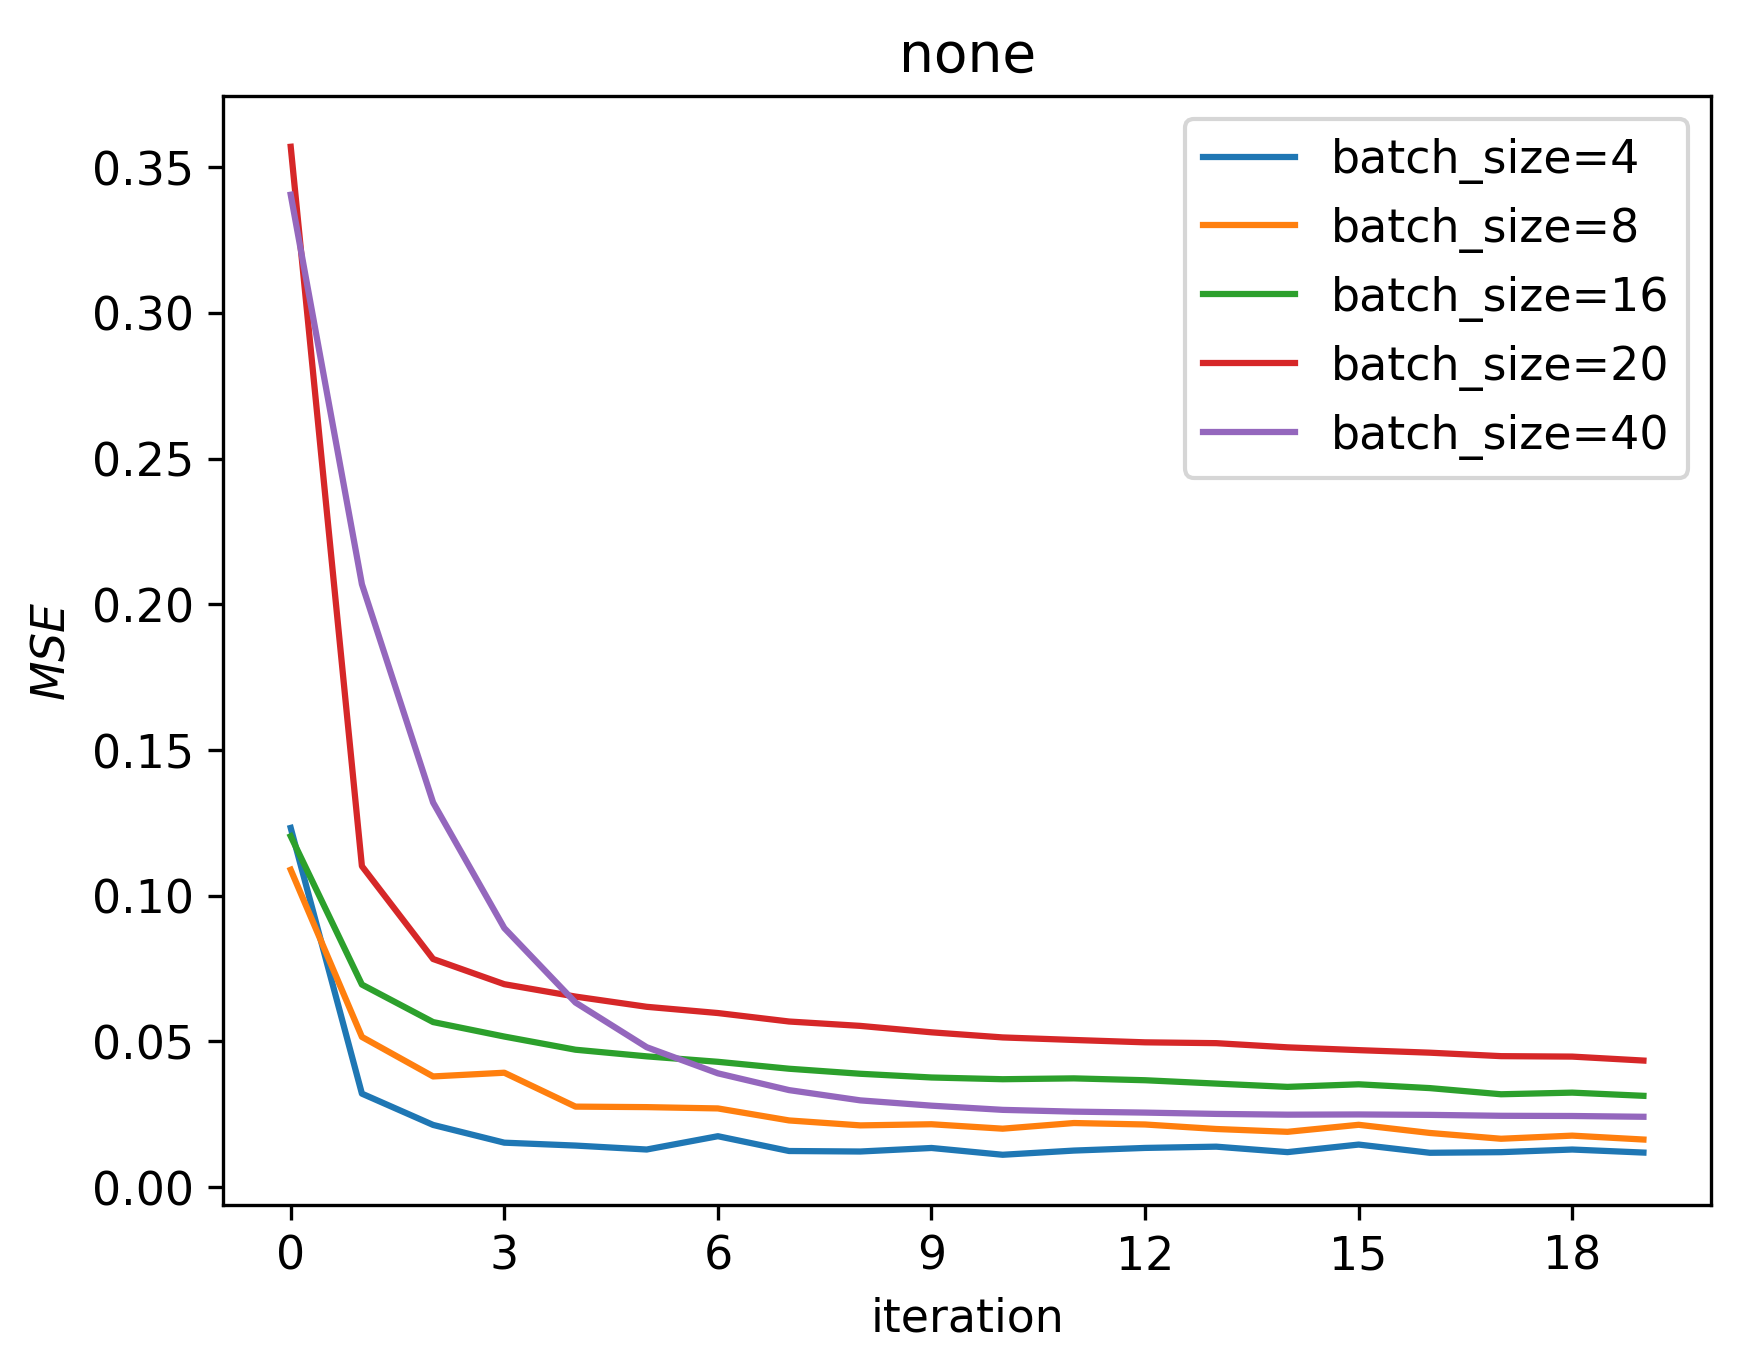
\includegraphics[width=.9\textwidth]{../figures/SGD_batch_size_none.png}
        \caption{no tune}
        \label{fig:}
    \end{subfigure}
    \begin{subfigure}{.5\textwidth}
        \centering
        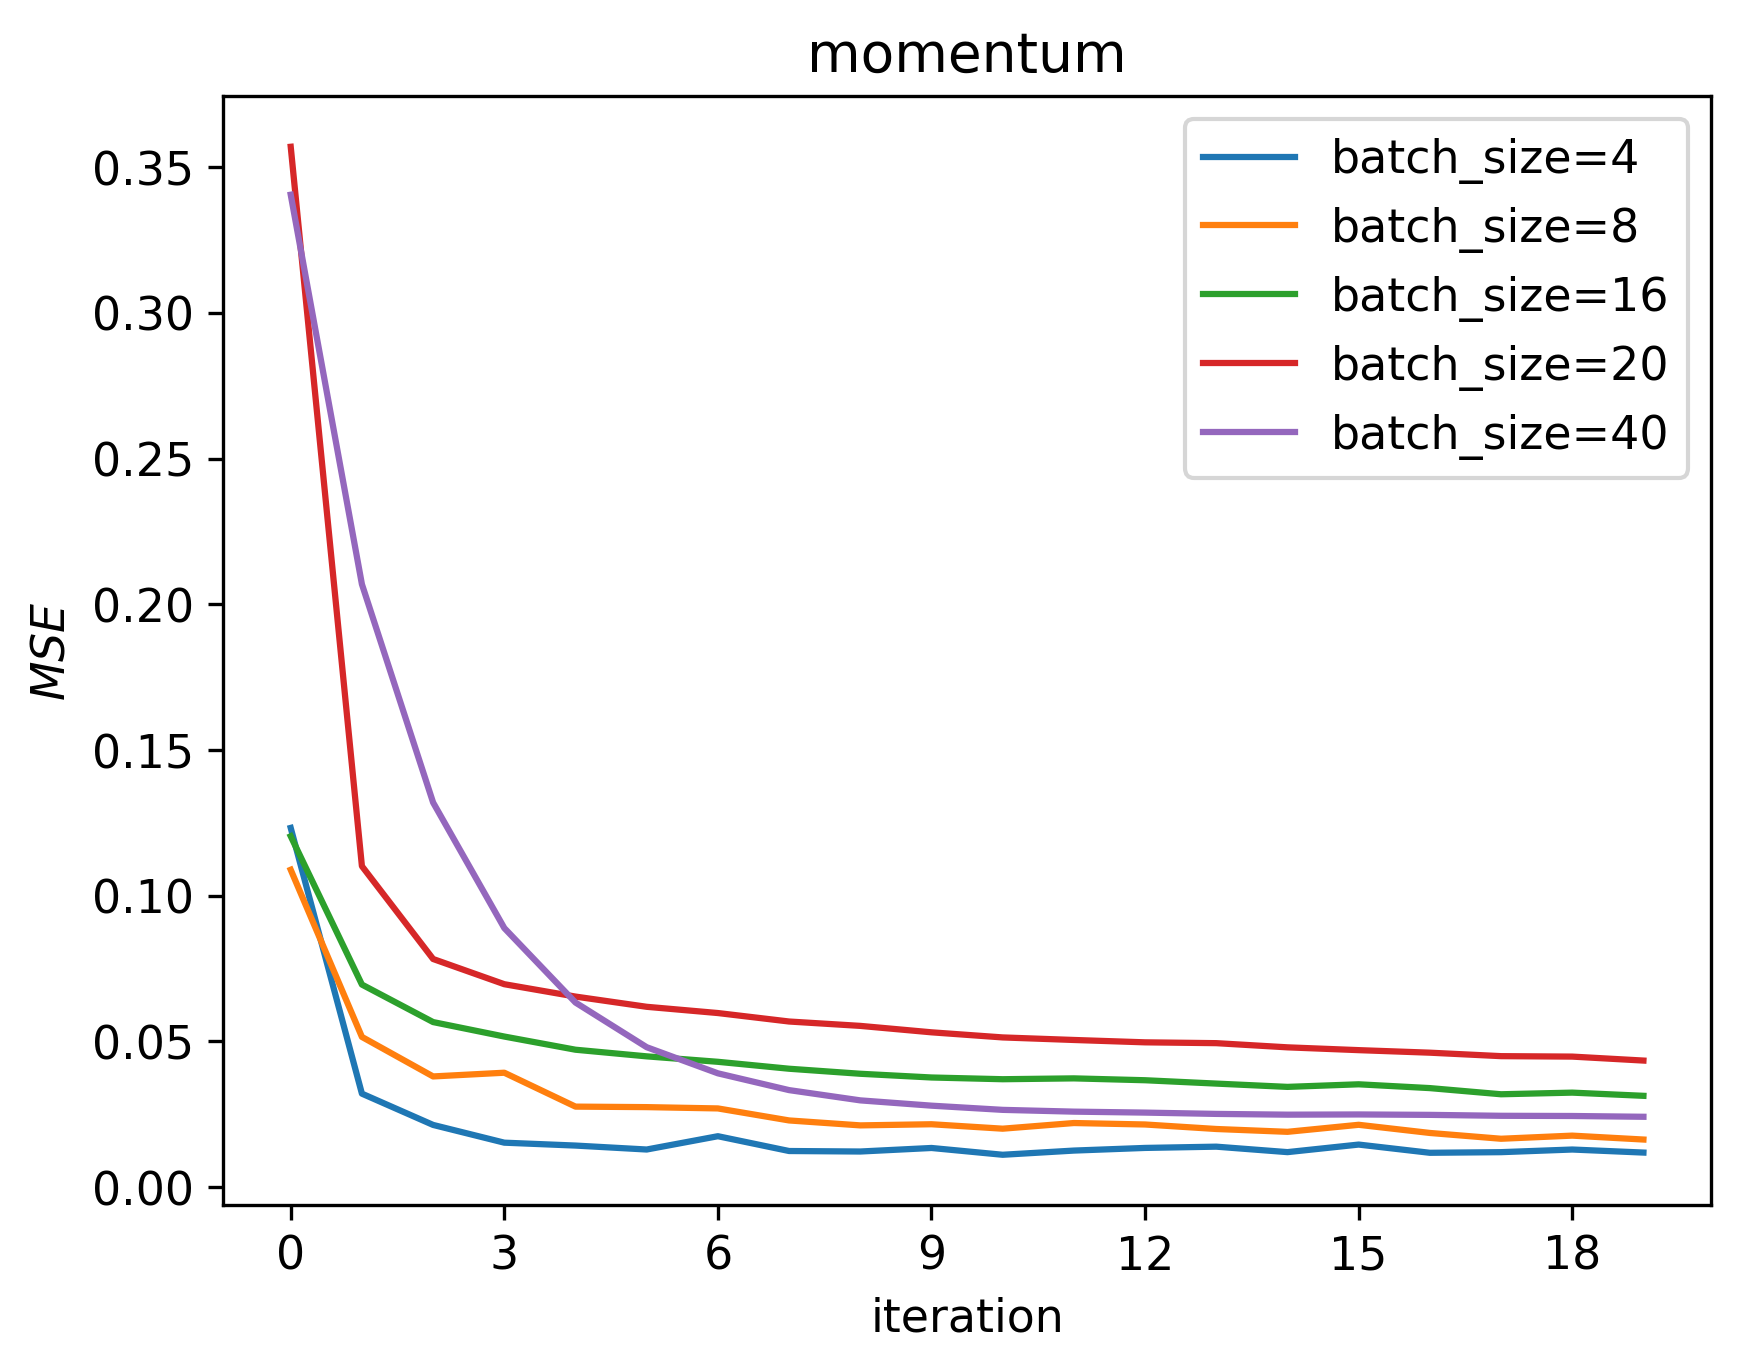
\includegraphics[width=.9\textwidth]{../figures/SGD_batch_size_momentum.png}
        \caption{momentum}
        \label{fig:}
    \end{subfigure}
    \begin{subfigure}{.5\textwidth}
        \centering
        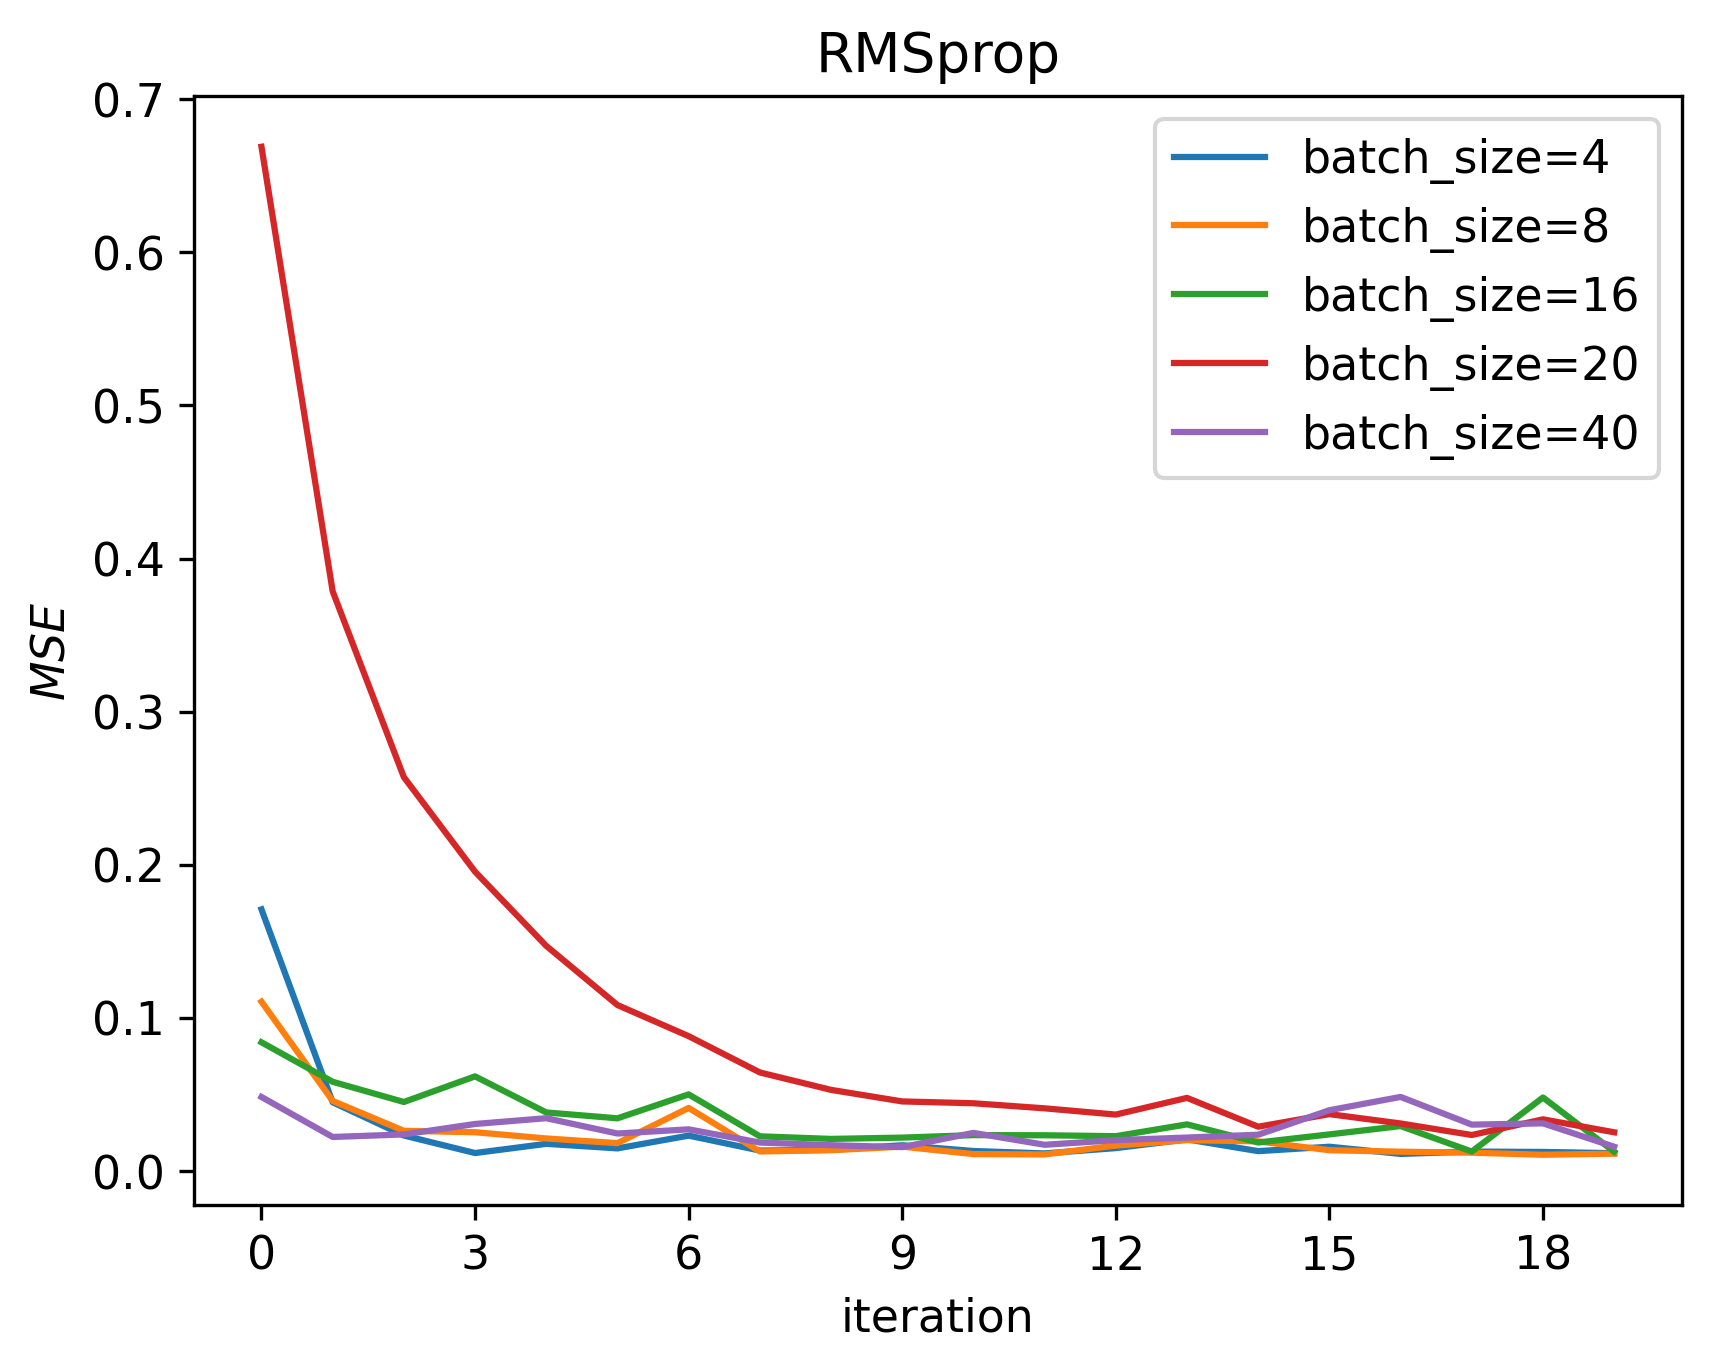
\includegraphics[width=.9\textwidth]{../figures/SGD_batch_size_RMSprop.png}
        \caption{RMSprop}
        \label{fig:}
    \end{subfigure}
    \begin{subfigure}{.9\textwidth}
        \centering
        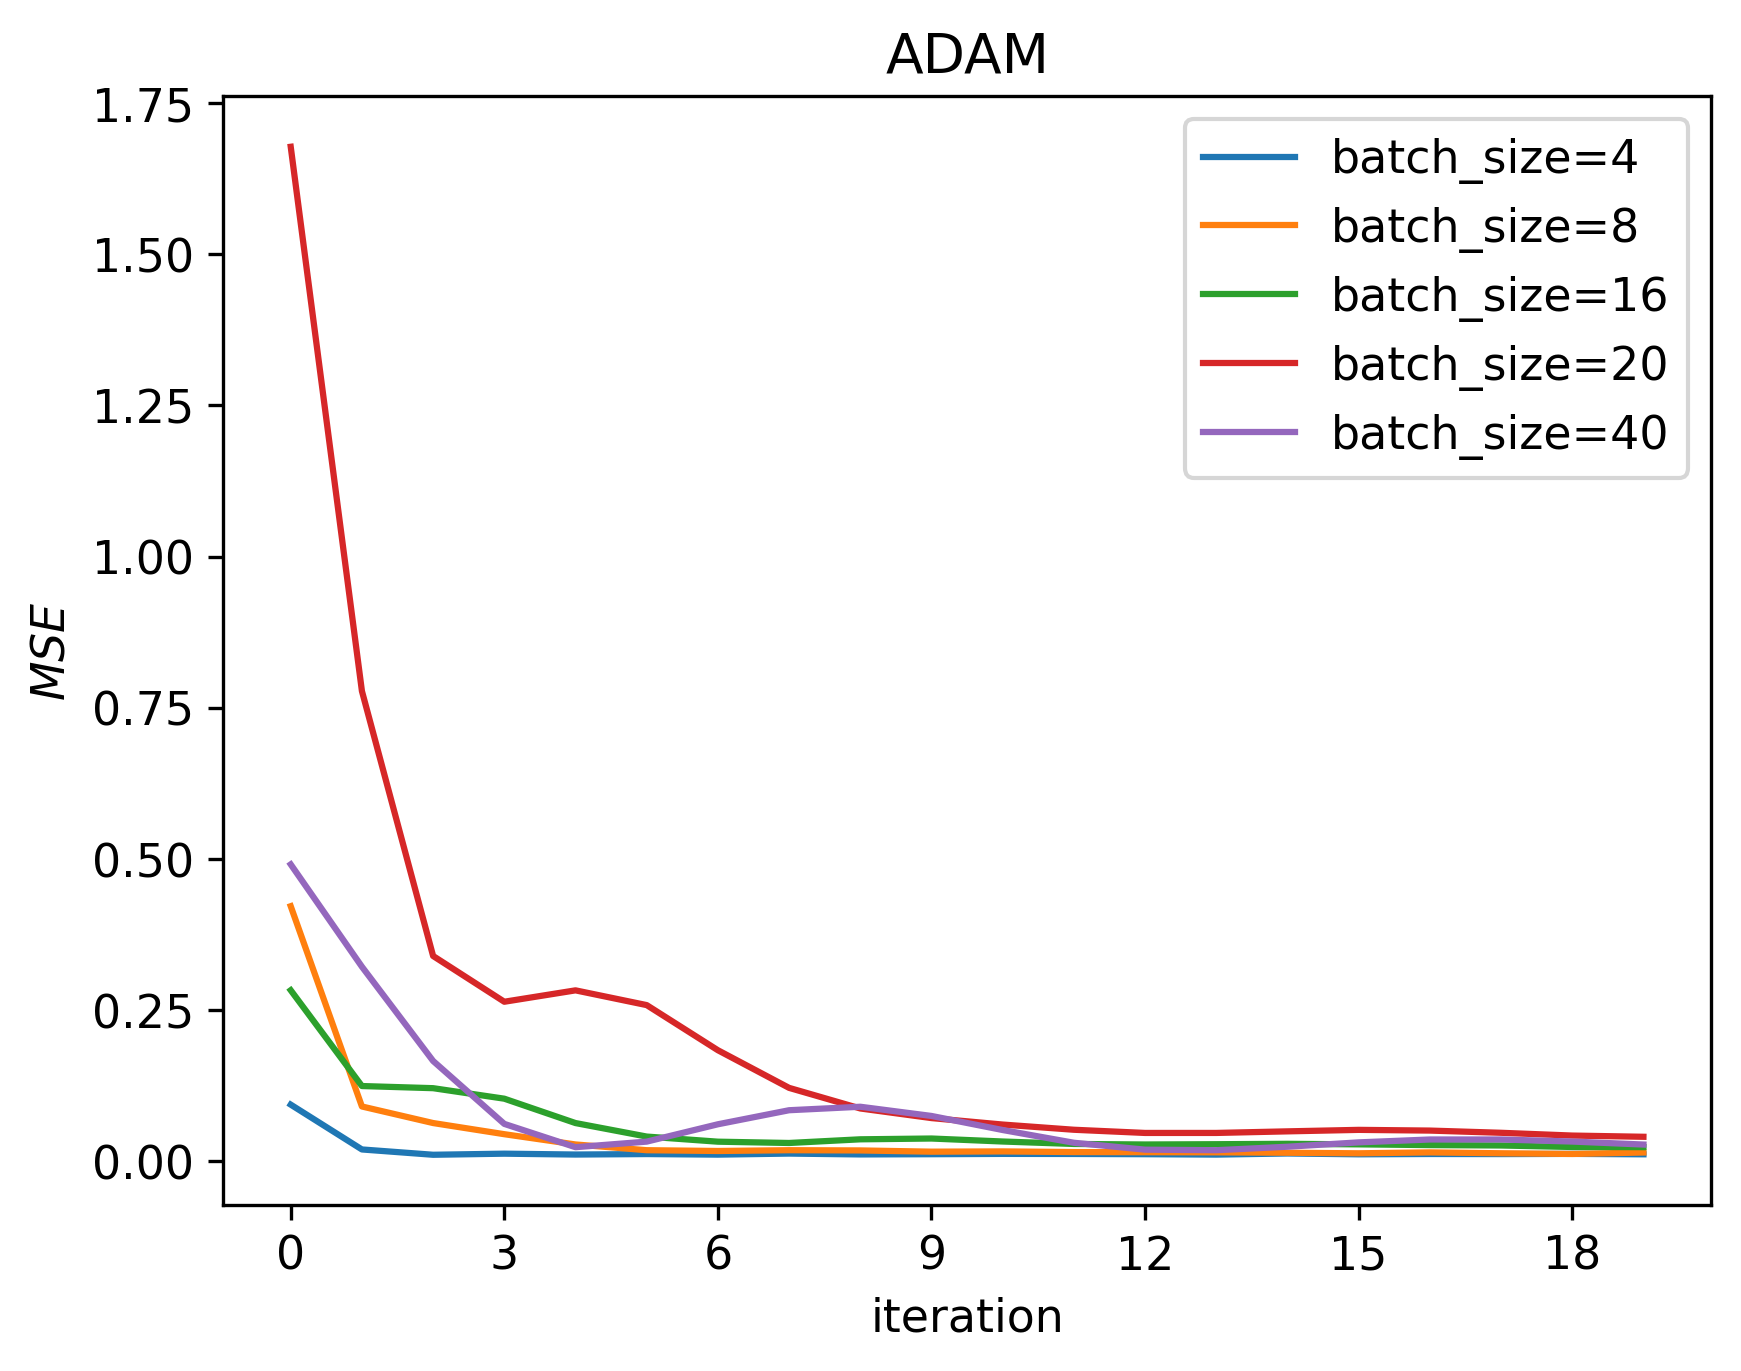
\includegraphics[width=.5\textwidth]{../figures/SGD_batch_size_ADAM.png}
        \caption{ADAM}
        \label{fig:}
    \end{subfigure}
    \caption{$MSE$ for different tuning functions and batch sizes for SGD.}
    \label{fig:compare_batch_size}
\end{figure}
In figure \ref{fig:compare_batch_size} we see that the convergence of SGD is greatly influenced by the batch size. We see that a batch size of 20 generally performs worse and that a lower batch size equals a faster convergence.

\subsection{Neural Network and the Franke function}
A grid search for our own neural network on the Franke function can be seen in figure \ref{fig:franke_grid} for sigmoid as activation function. Grid search using ReLU can be seen in figure \ref{fig:franke_grid_2} and figure \ref{fig:franke_grid_3} is for the leaky ReLU
\begin{figure}[H]
    \begin{subfigure}{.5\textwidth}
        \centering
        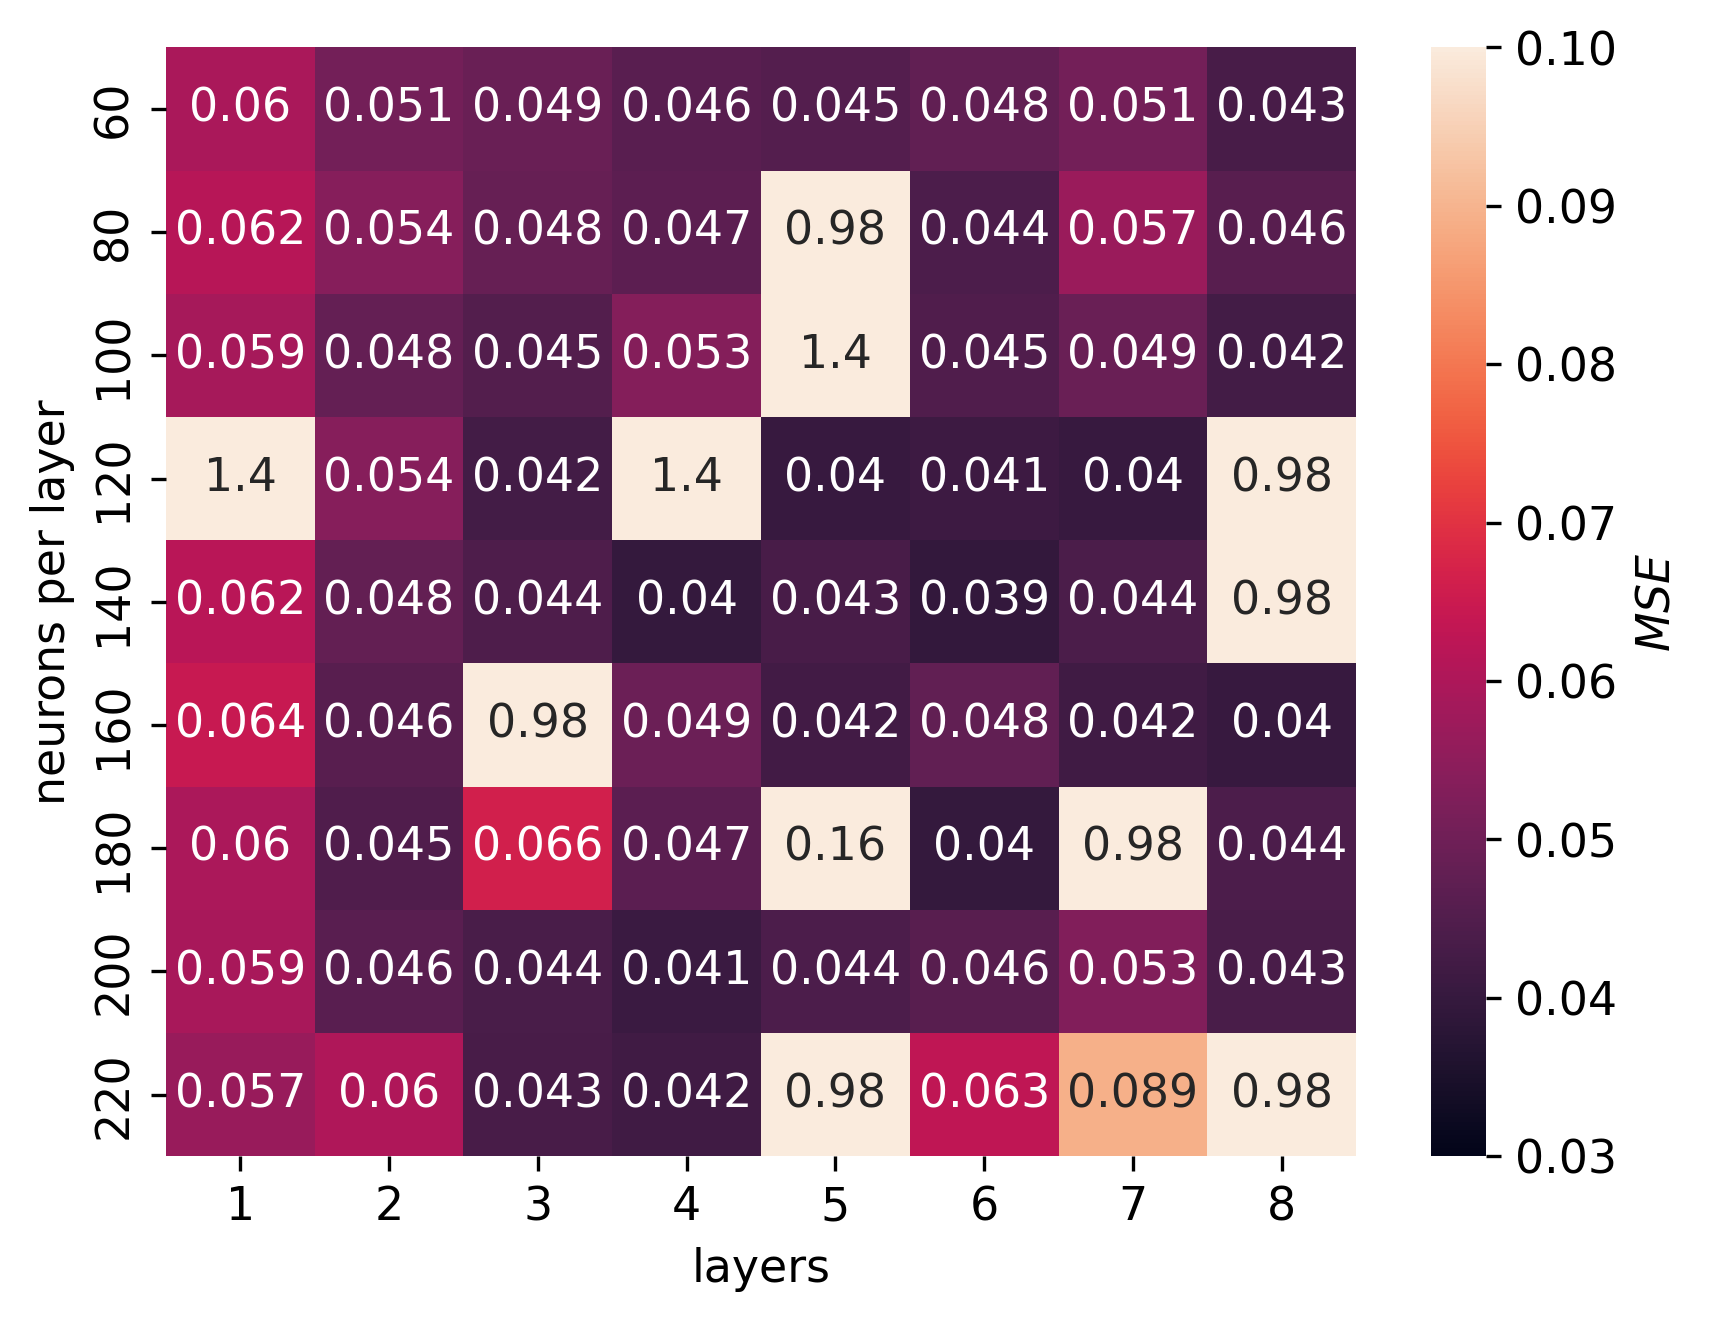
\includegraphics[width=\textwidth]{../figures/franke_L_n_test_sigmoid.png}
        \caption{$MSE$ for number of layers vs number of neurons}
        \label{fig:}
    \end{subfigure}
    \begin{subfigure}{.5\textwidth}
        \centering
        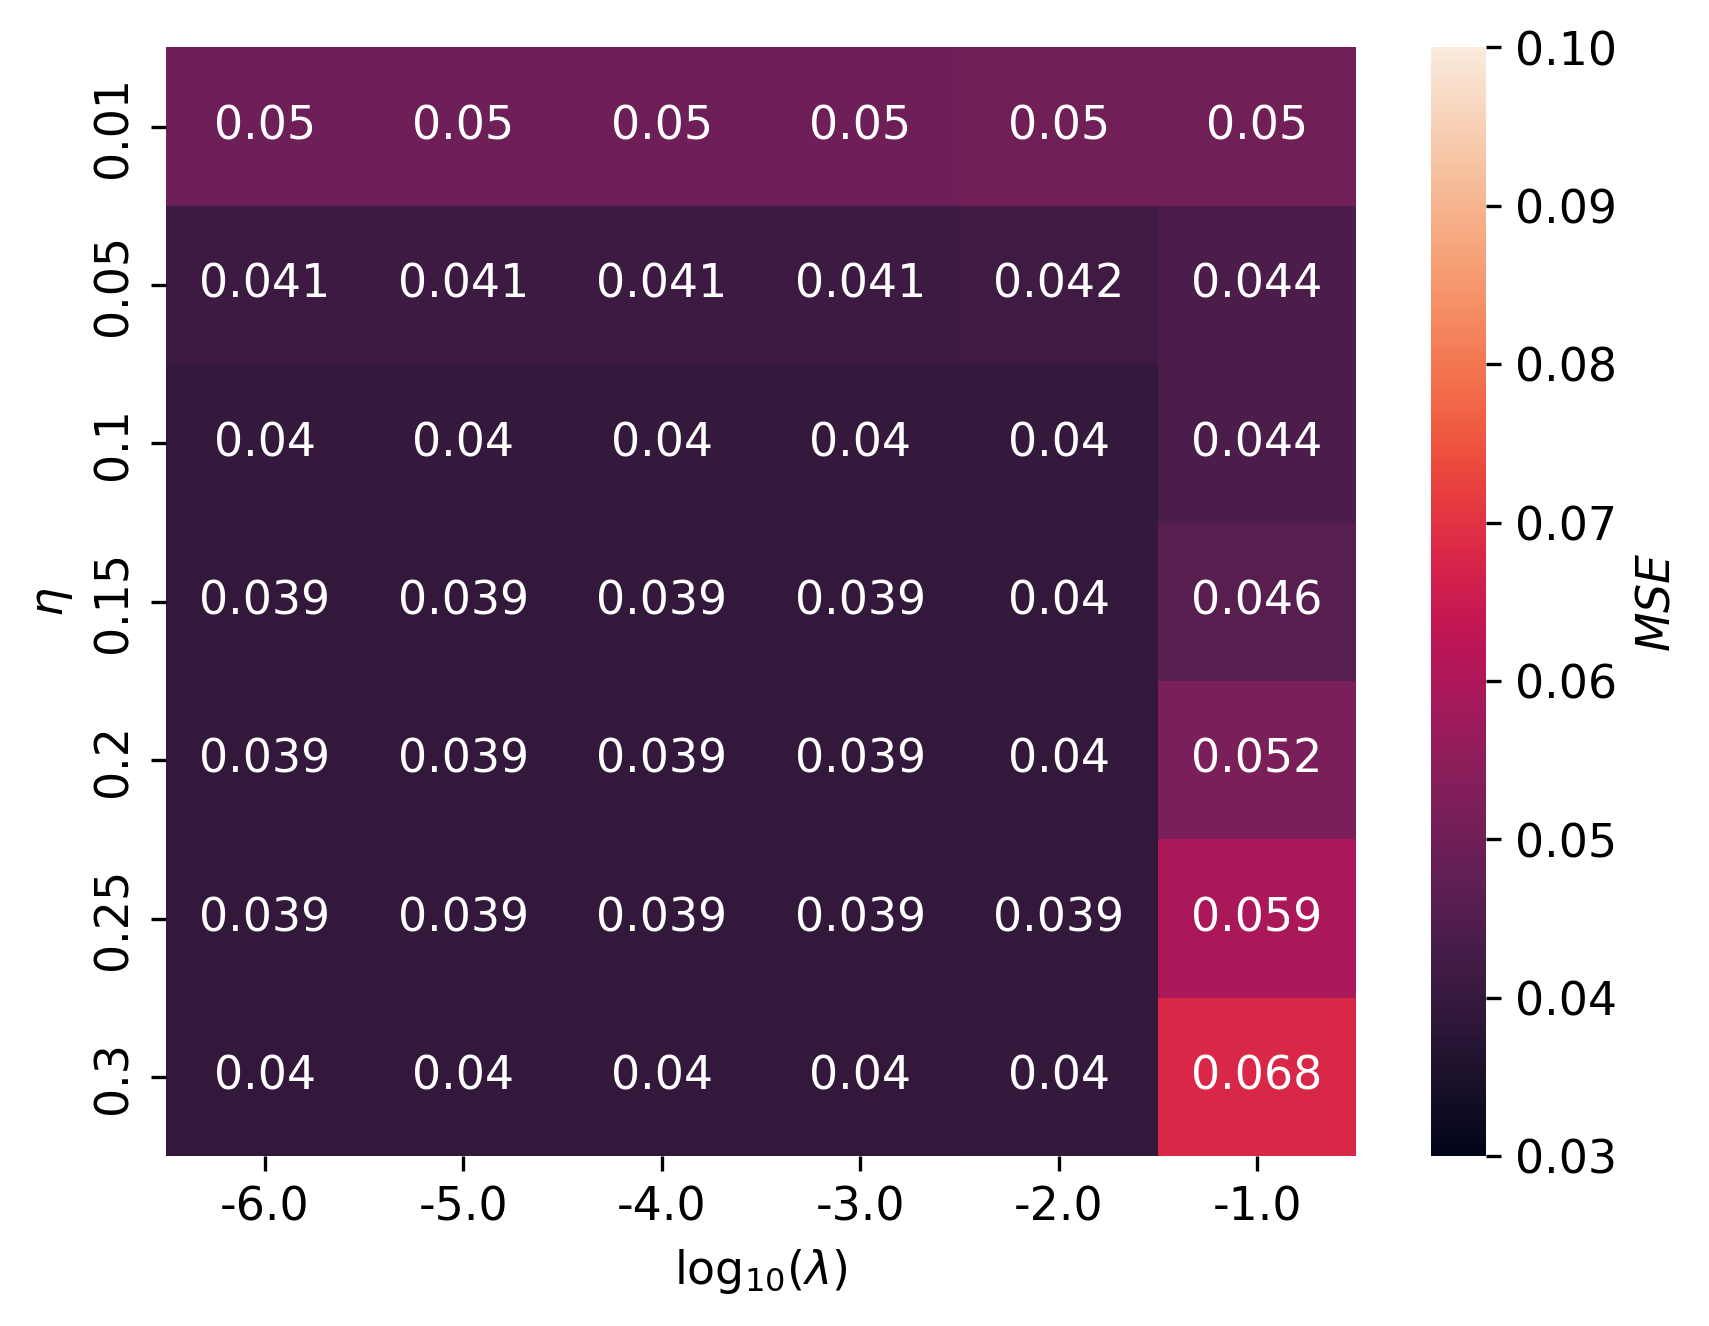
\includegraphics[width=\textwidth]{../figures/franke_eta_lmb_sigmoid.png}
        \caption{$MSE$ for $\eta$ vs $\lambda$}
        \label{fig:}
    \end{subfigure}
    \begin{subfigure}{.5\textwidth}
        \centering
        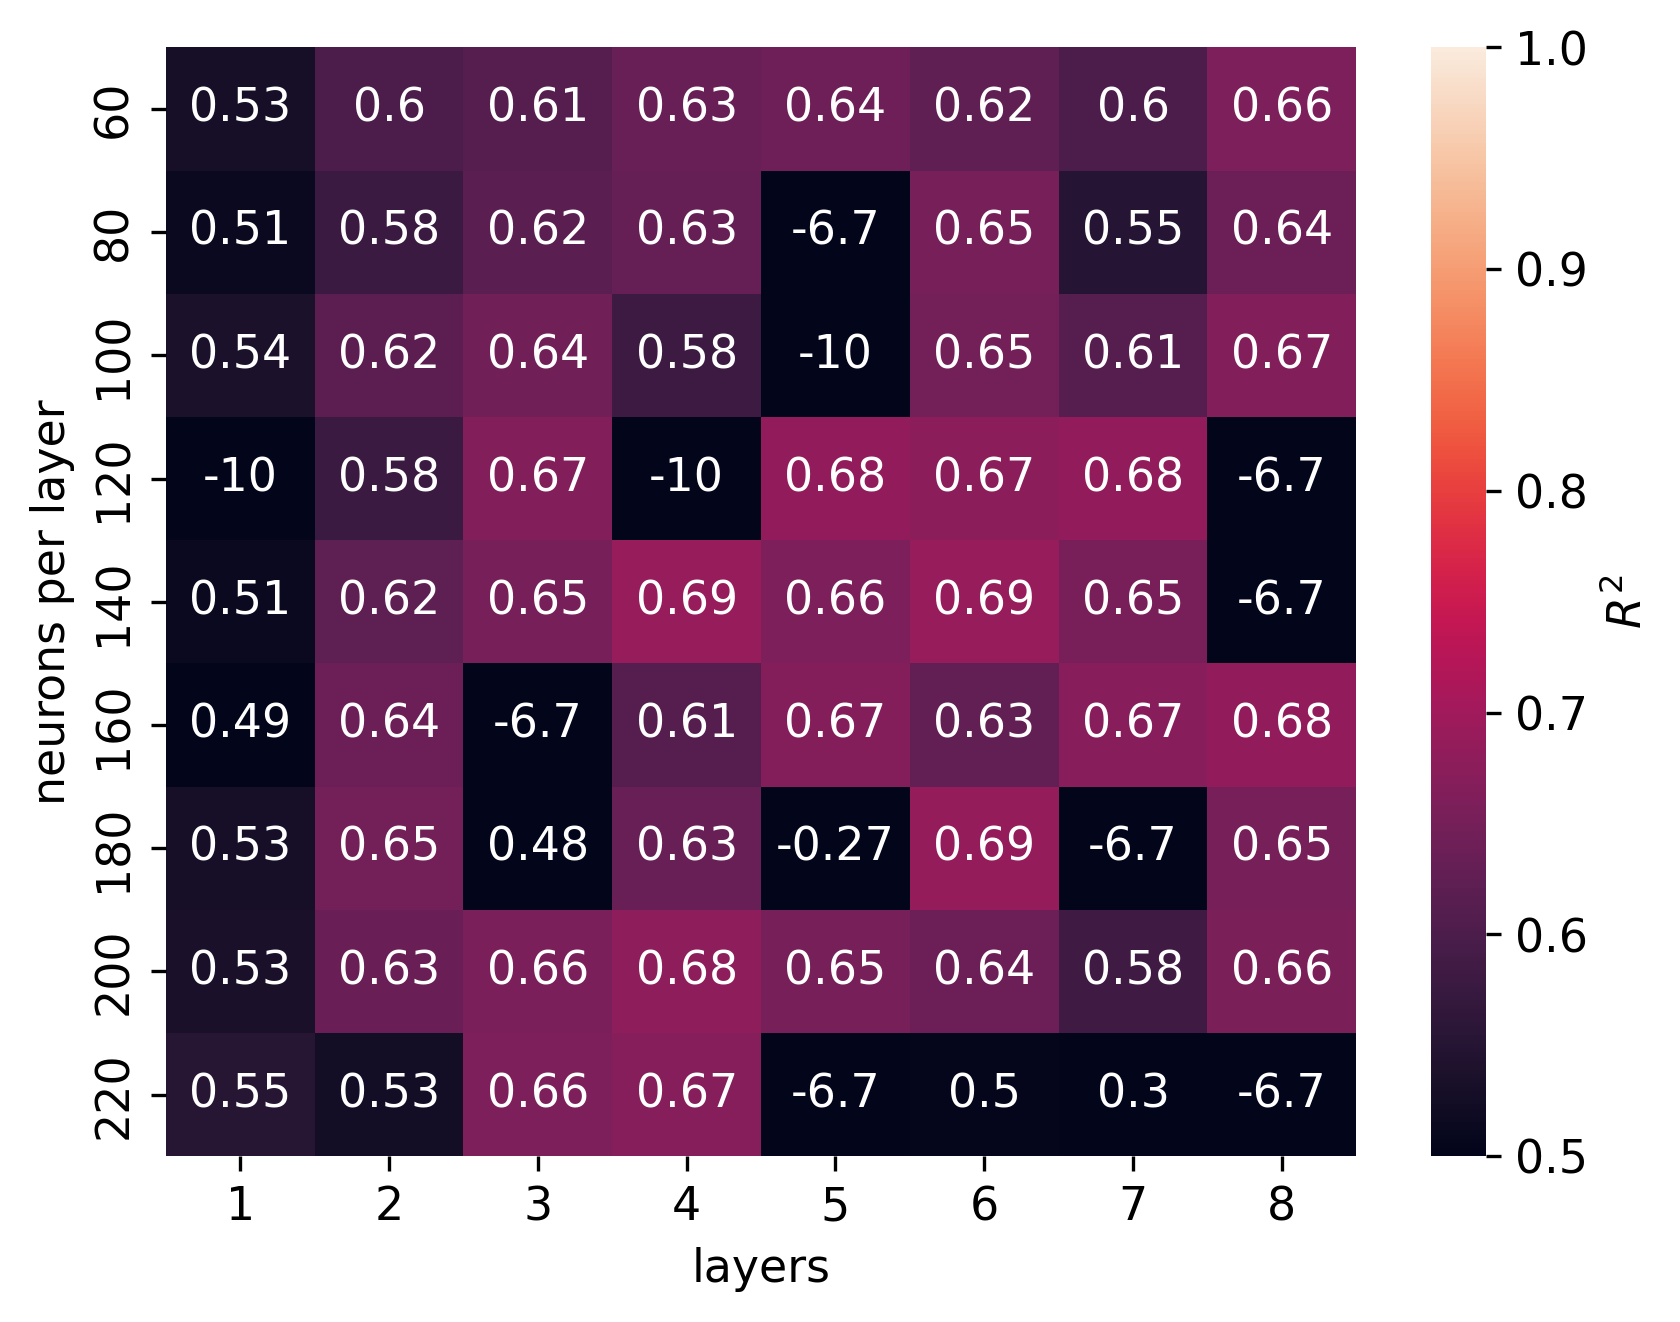
\includegraphics[width=\textwidth]{../figures/franke_L_n_test_sigmoid_R2.png}
        \caption{$R^2$ for number of layers vs number of neurons}
        \label{fig:}
    \end{subfigure}
    \begin{subfigure}{.5\textwidth}
        \centering
        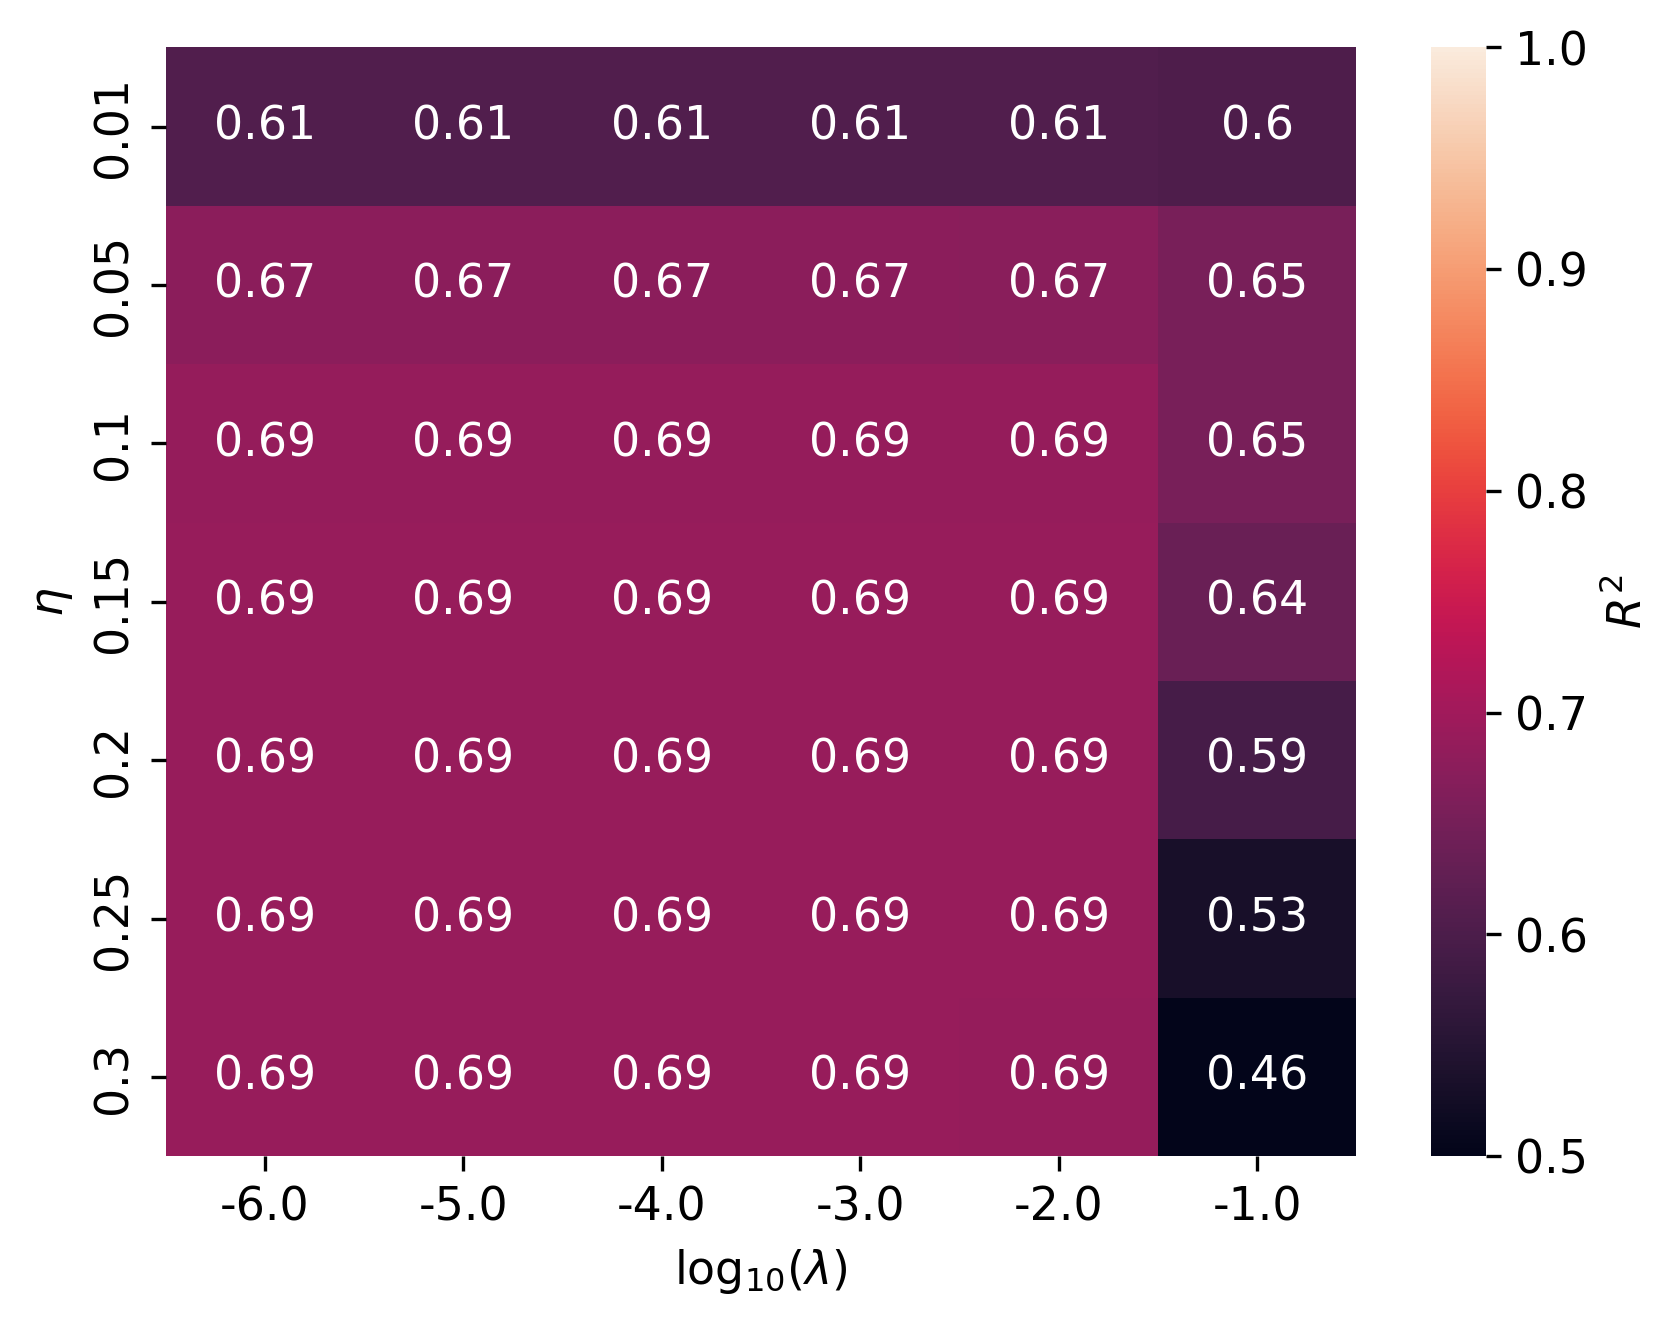
\includegraphics[width=\textwidth]{../figures/franke_eta_lmb_sigmoid_R2.png}
        \caption{$R^2$ for $\eta$ vs $\lambda$}
        \label{fig:}
    \end{subfigure}
    \caption{$MSE$ and $R^2$ grid search for Franke function to find the best possible $\eta$, $\lambda$, number of layers and number of neurons for sigmoid as activation function}
    \label{fig:franke_grid}
\end{figure}
\begin{figure}[H]
    \begin{subfigure}{.5\textwidth}
        \centering
        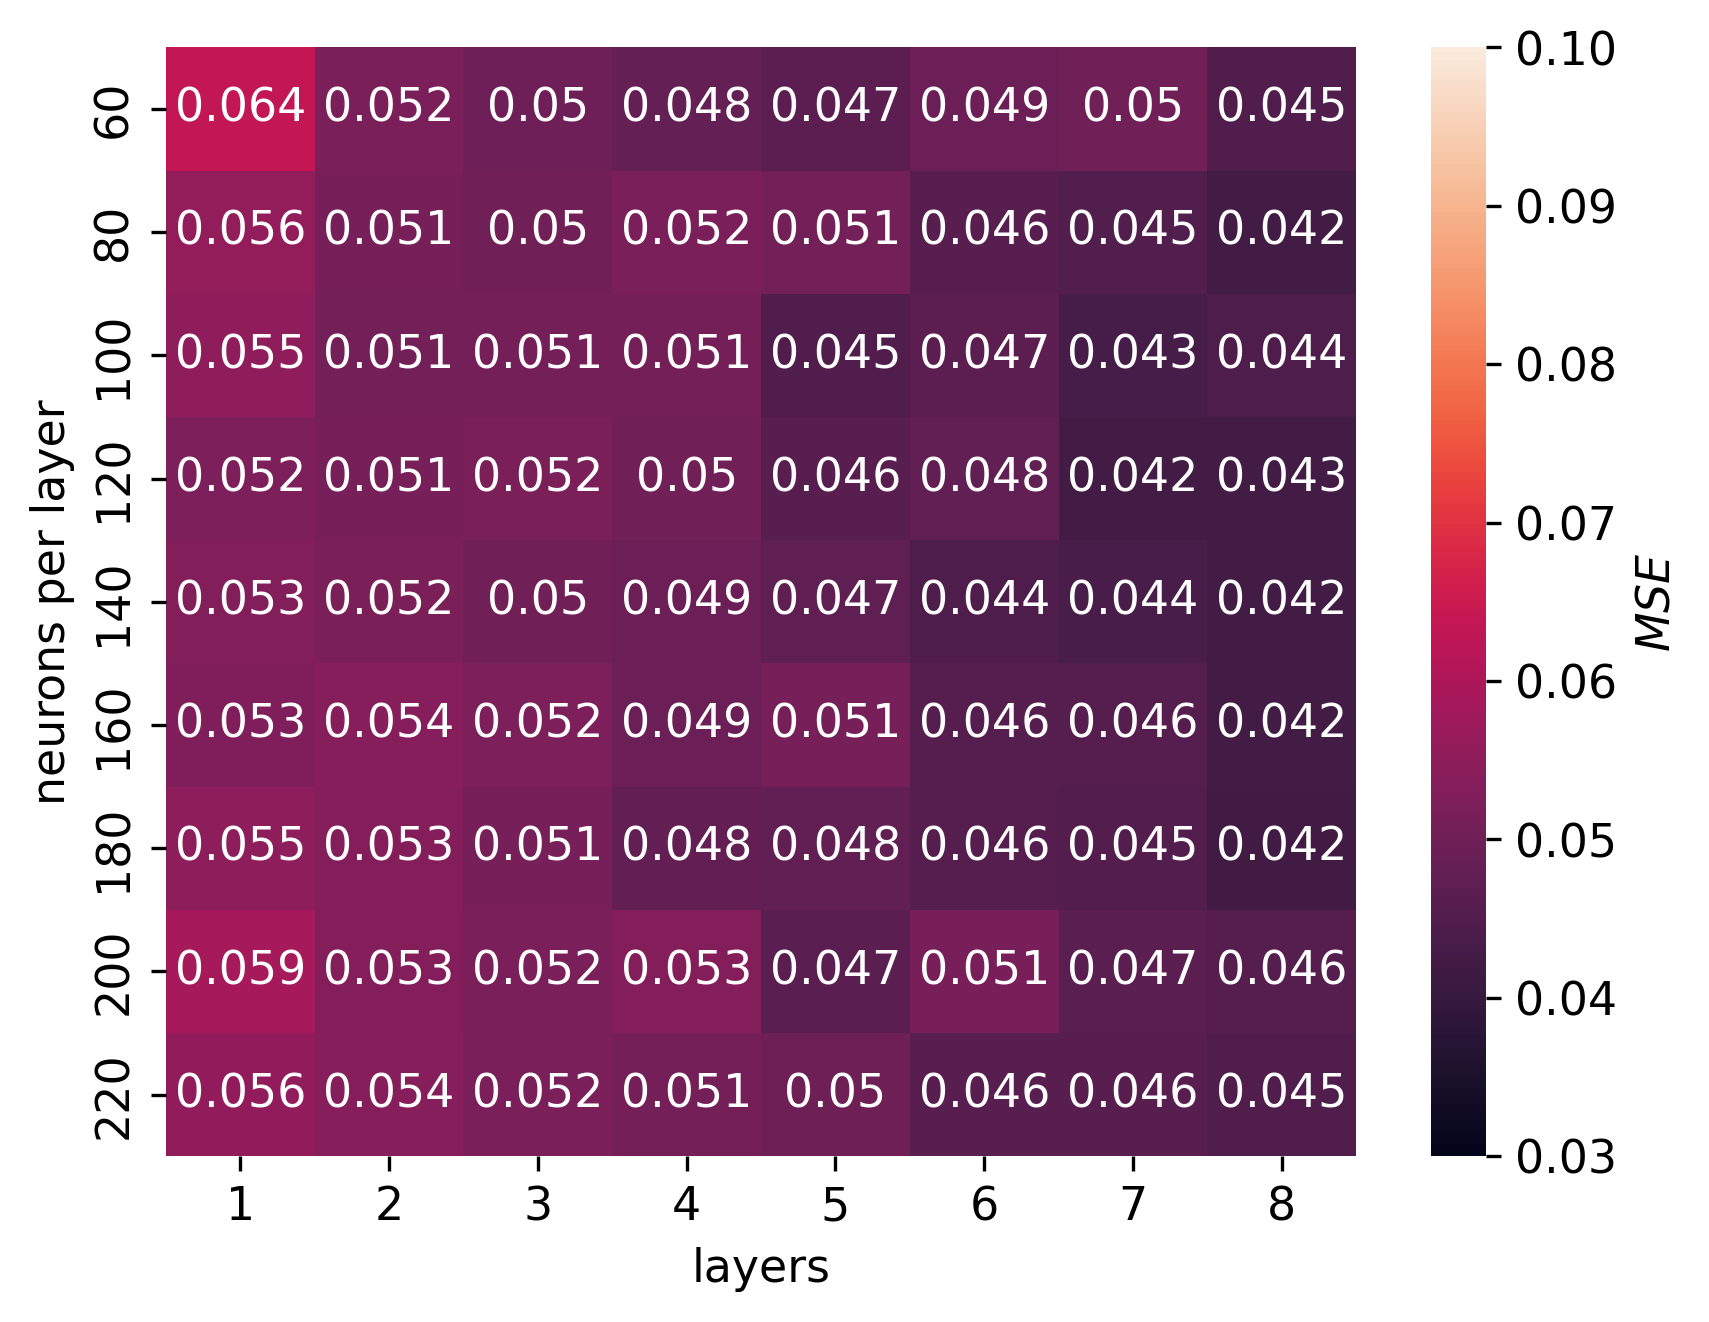
\includegraphics[width=\textwidth]{../figures/franke_L_n_test_relu_MSE.png}
        \caption{$MSE$ for number of layers vs number of neurons}
        \label{fig:}
    \end{subfigure}
    \begin{subfigure}{.5\textwidth}
        \centering
        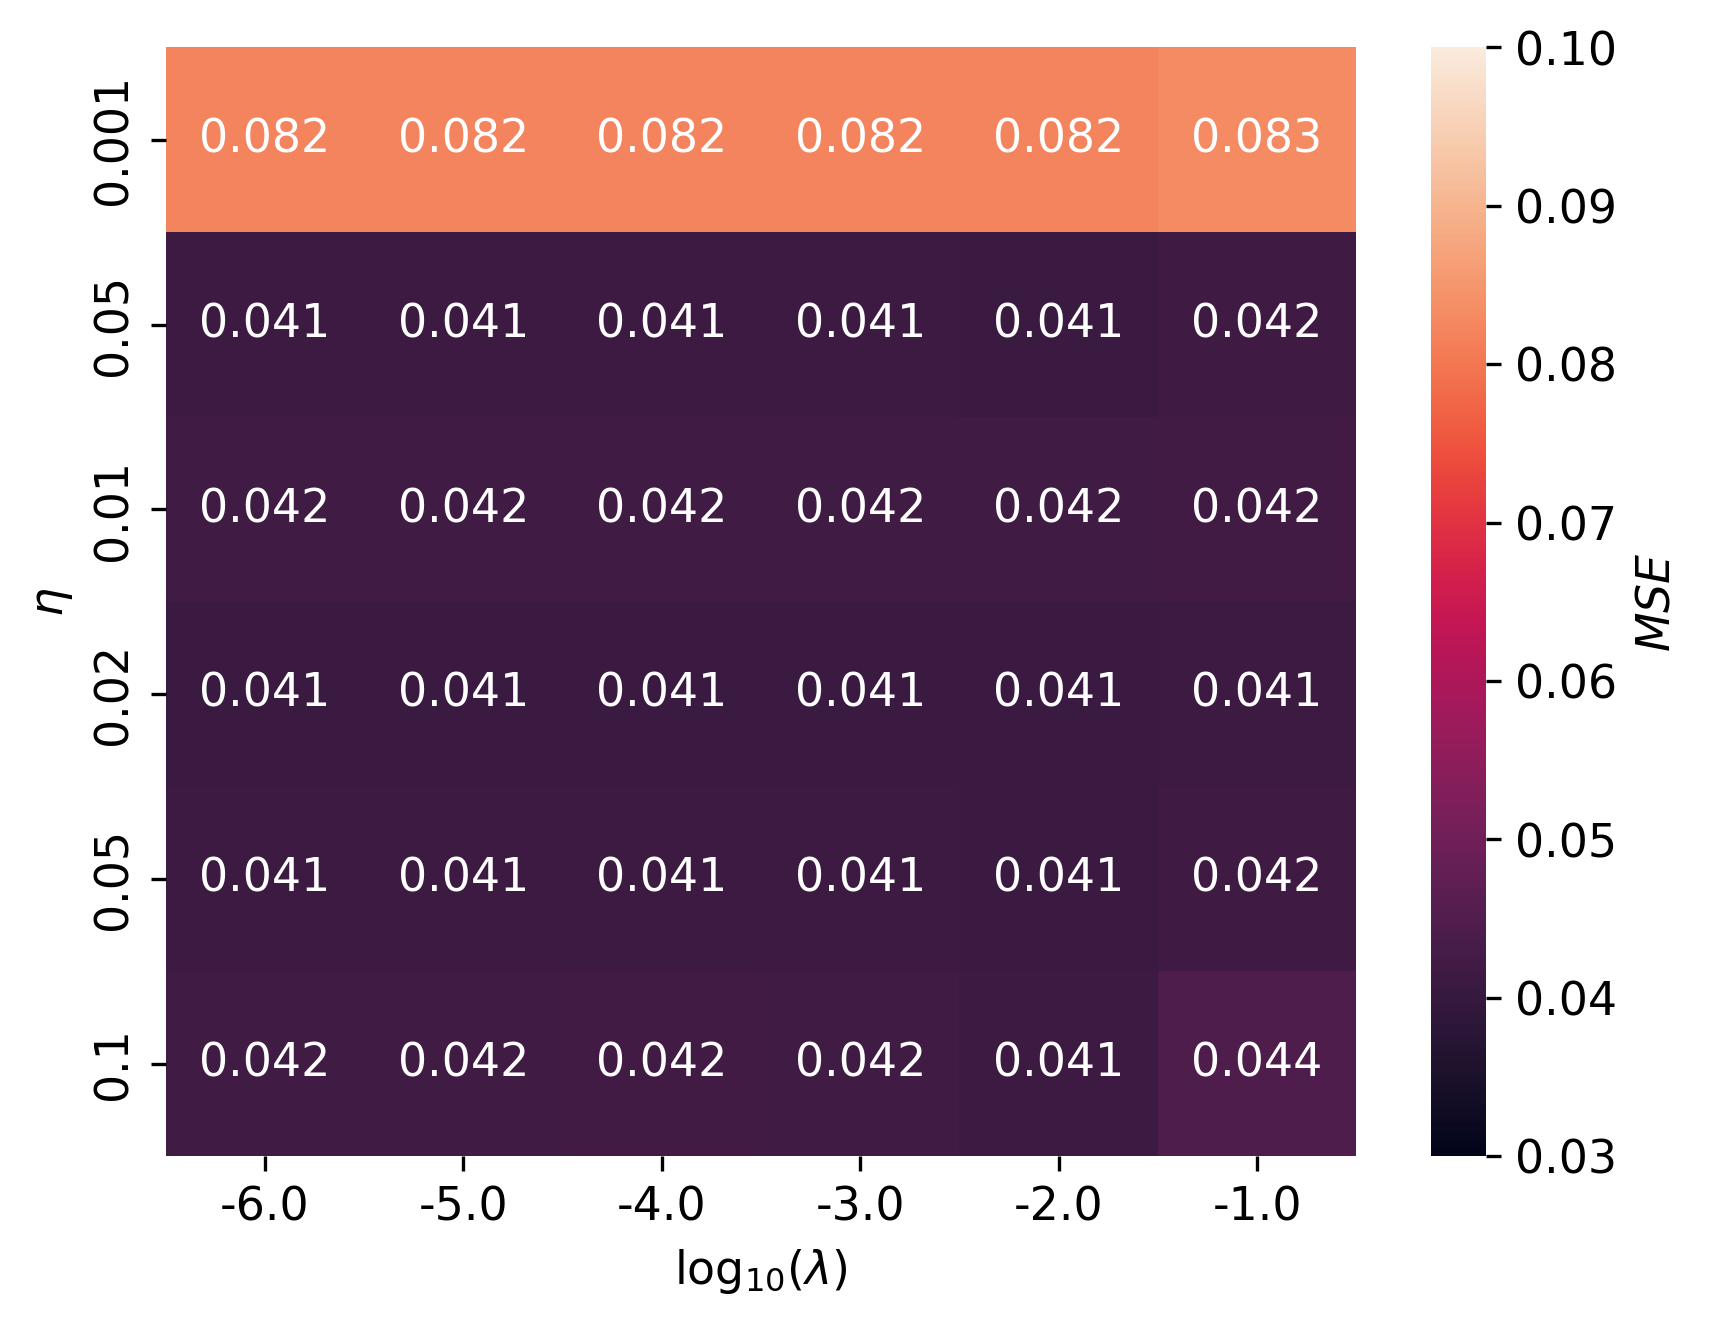
\includegraphics[width=\textwidth]{../figures/franke_eta_lmb_relu.png}
        \caption{$MSE$ for $\eta$ vs $\lambda$}
        \label{fig:}
    \end{subfigure}
    \begin{subfigure}{.5\textwidth}
        \centering
        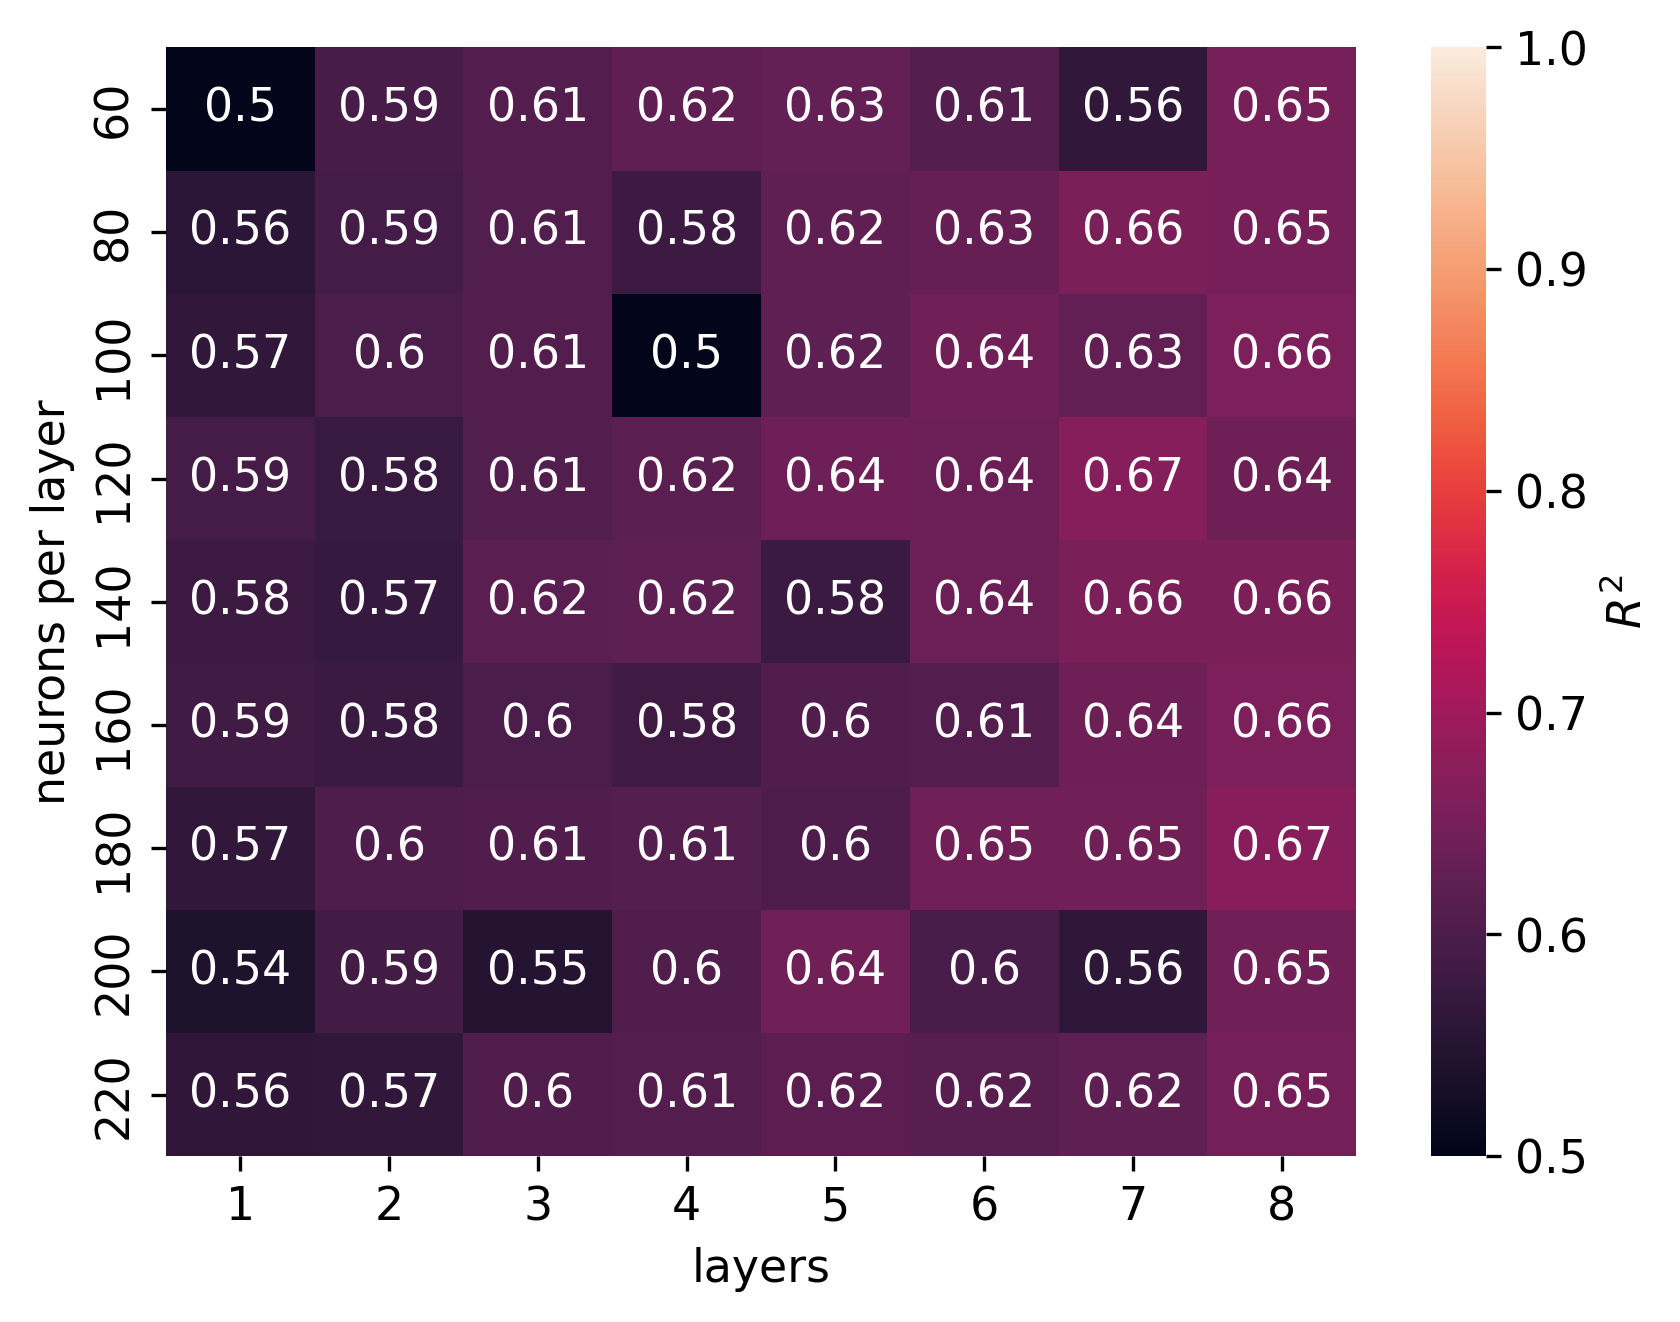
\includegraphics[width=\textwidth]{../figures/franke_L_n_test_relu_R2.png}
        \caption{$R^2$ for number of layers vs number of neurons}
        \label{fig:}
    \end{subfigure}
    \begin{subfigure}{.5\textwidth}
        \centering
        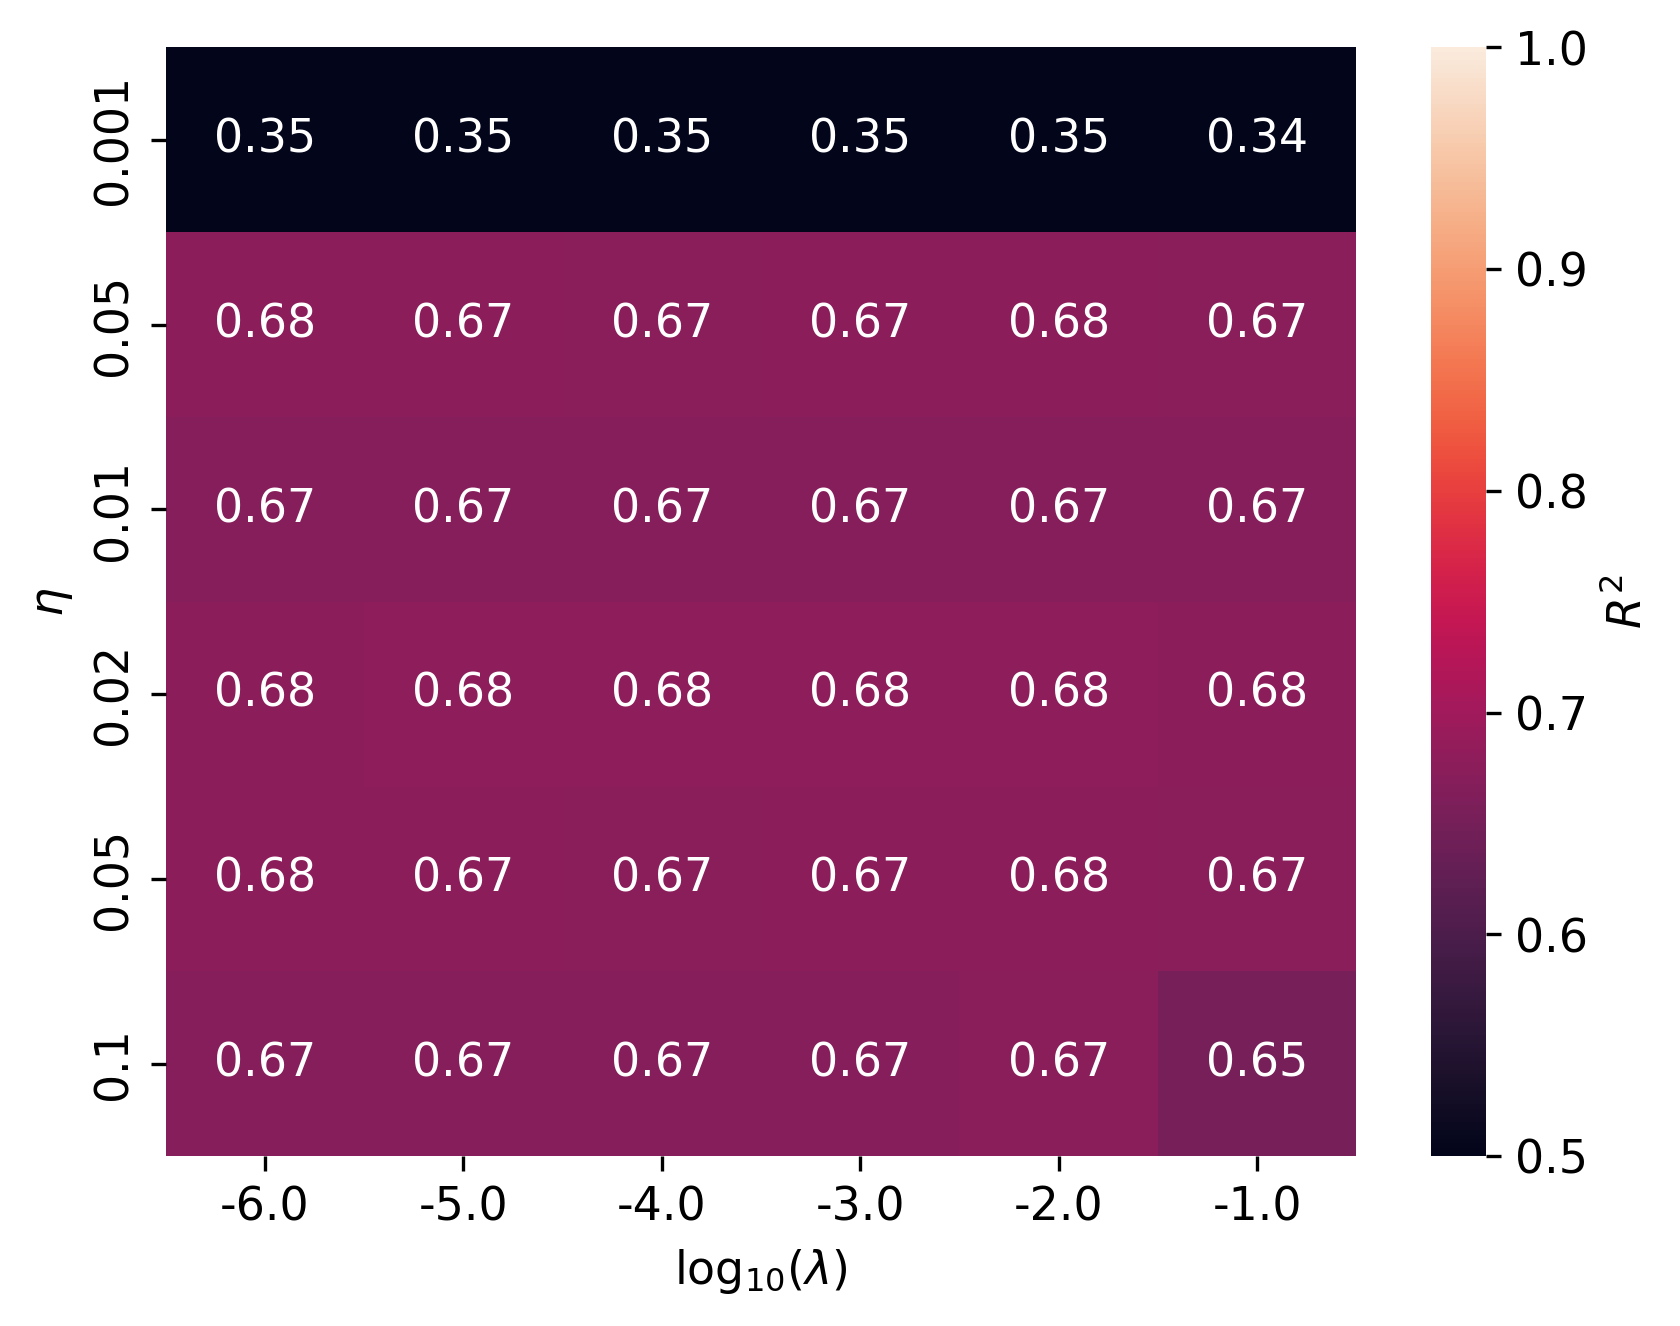
\includegraphics[width=\textwidth]{../figures/franke_eta_lmb_relu_R2.png}
        \caption{$R^2$ for $\eta$ vs $\lambda$}
        \label{fig:}
    \end{subfigure}
    \caption{$MSE$ and $R^2$ grid search for Franke function to find the best possible $\eta$, $\lambda$, number of layers and number of neurons for ReLU as activation function}
    \label{fig:franke_grid_2}
\end{figure}
\begin{figure}[H]
    \begin{subfigure}{.5\textwidth}
        \centering
        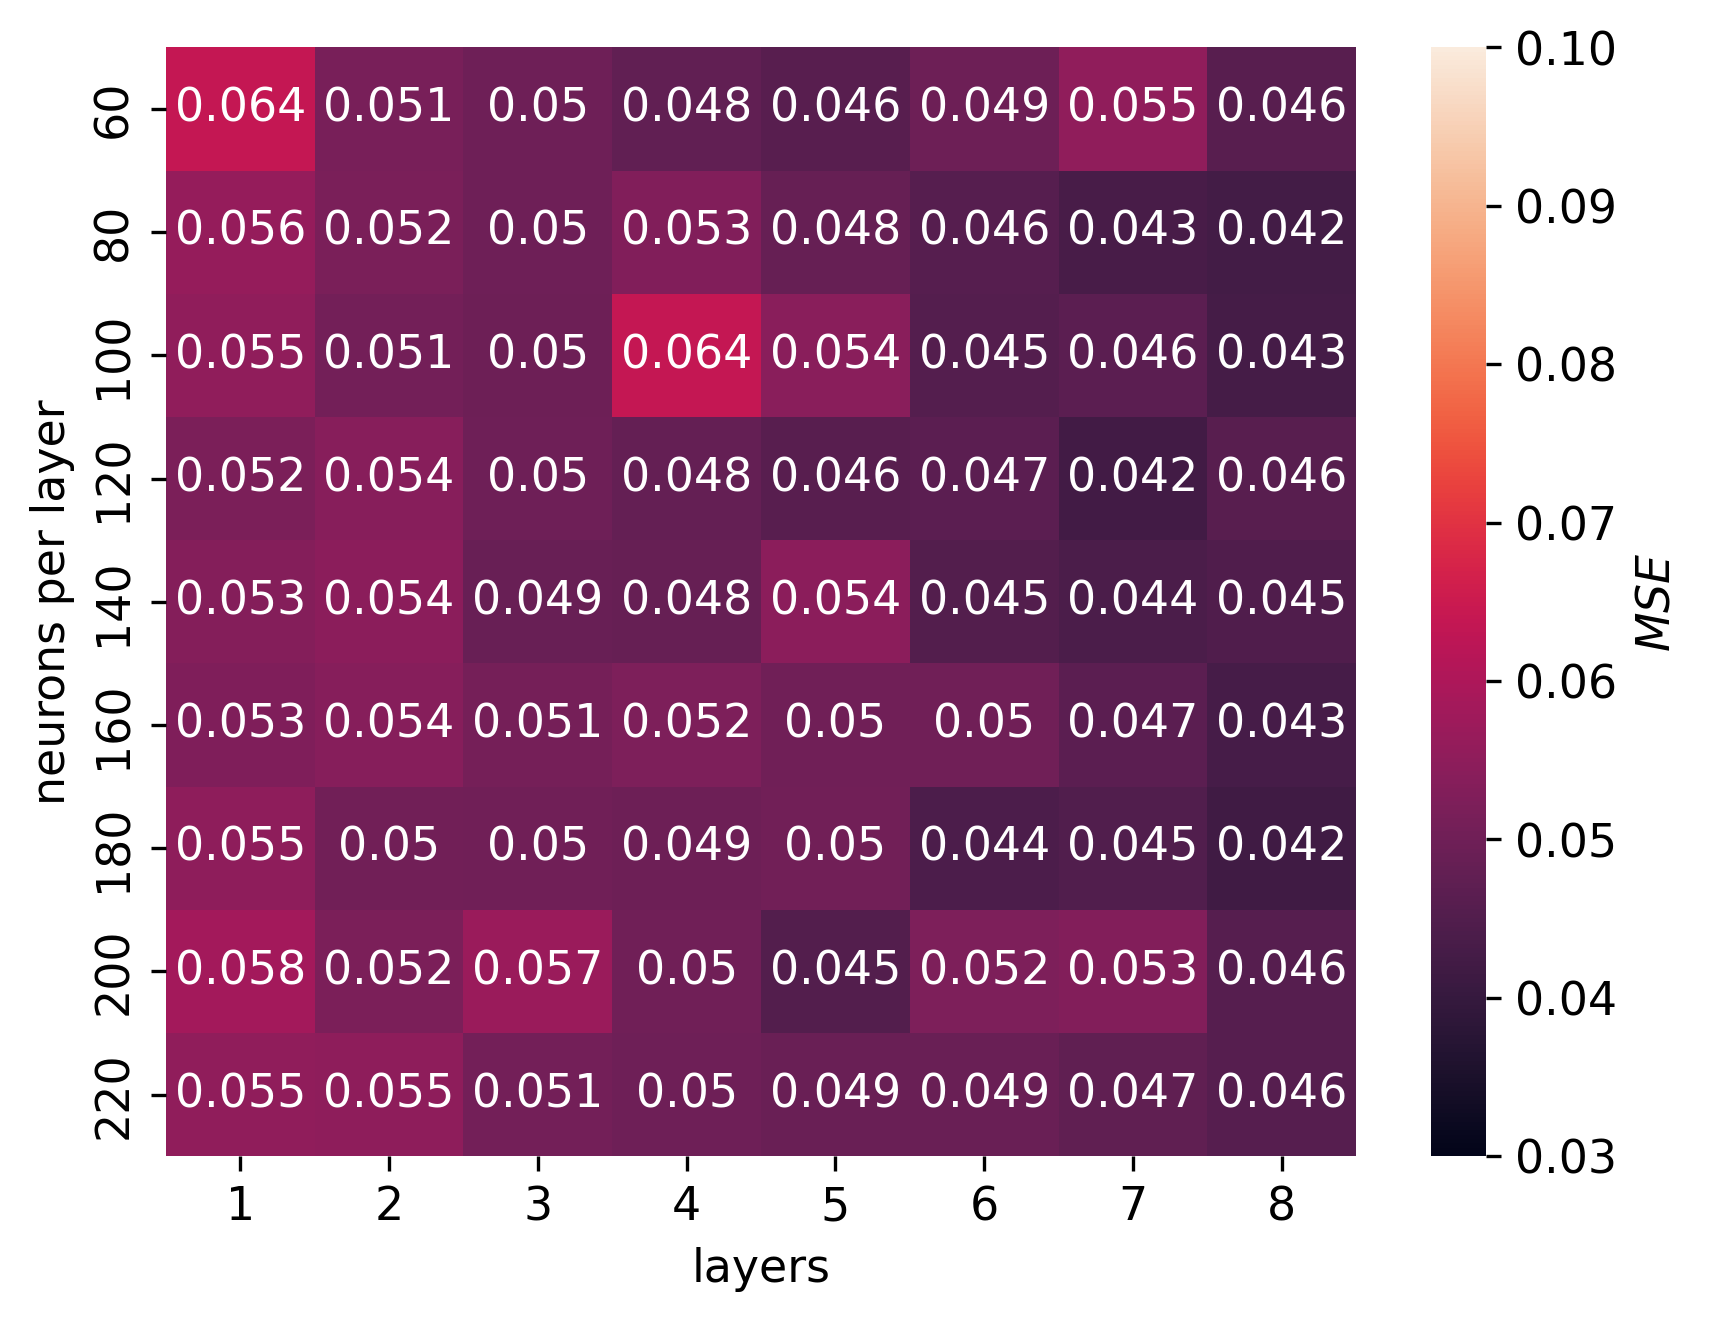
\includegraphics[width=\textwidth]{../figures/franke_L_n_test_lrelu_MSE.png}
        \caption{$MSE$ for number of layers vs number of neurons}
        \label{fig:}
    \end{subfigure}
    \begin{subfigure}{.5\textwidth}
        \centering
        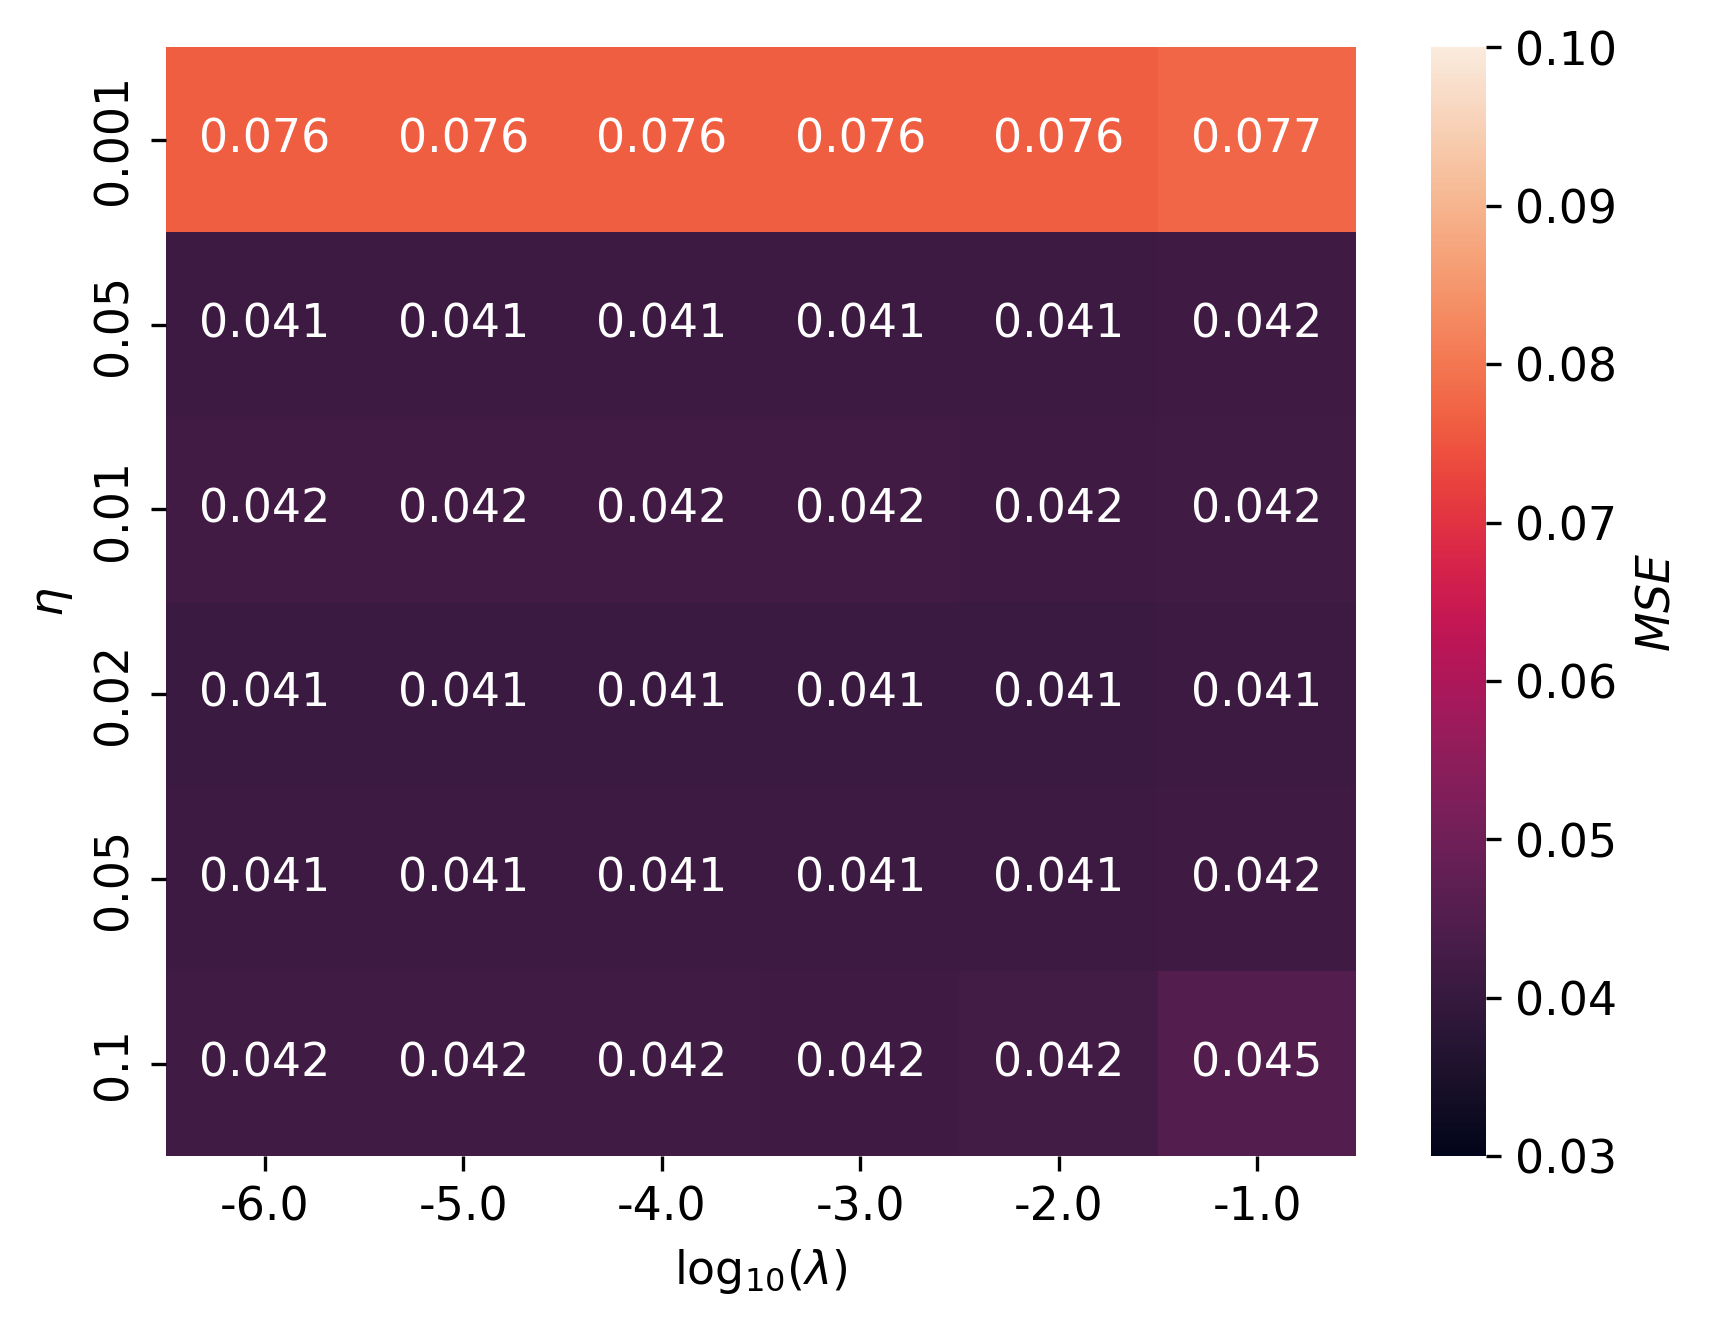
\includegraphics[width=\textwidth]{../figures/franke_eta_lmb_lrelu_MSE.png}
        \caption{$MSE$ for $\eta$ vs $\lambda$}
        \label{fig:}
    \end{subfigure}
    \begin{subfigure}{.5\textwidth}
        \centering
        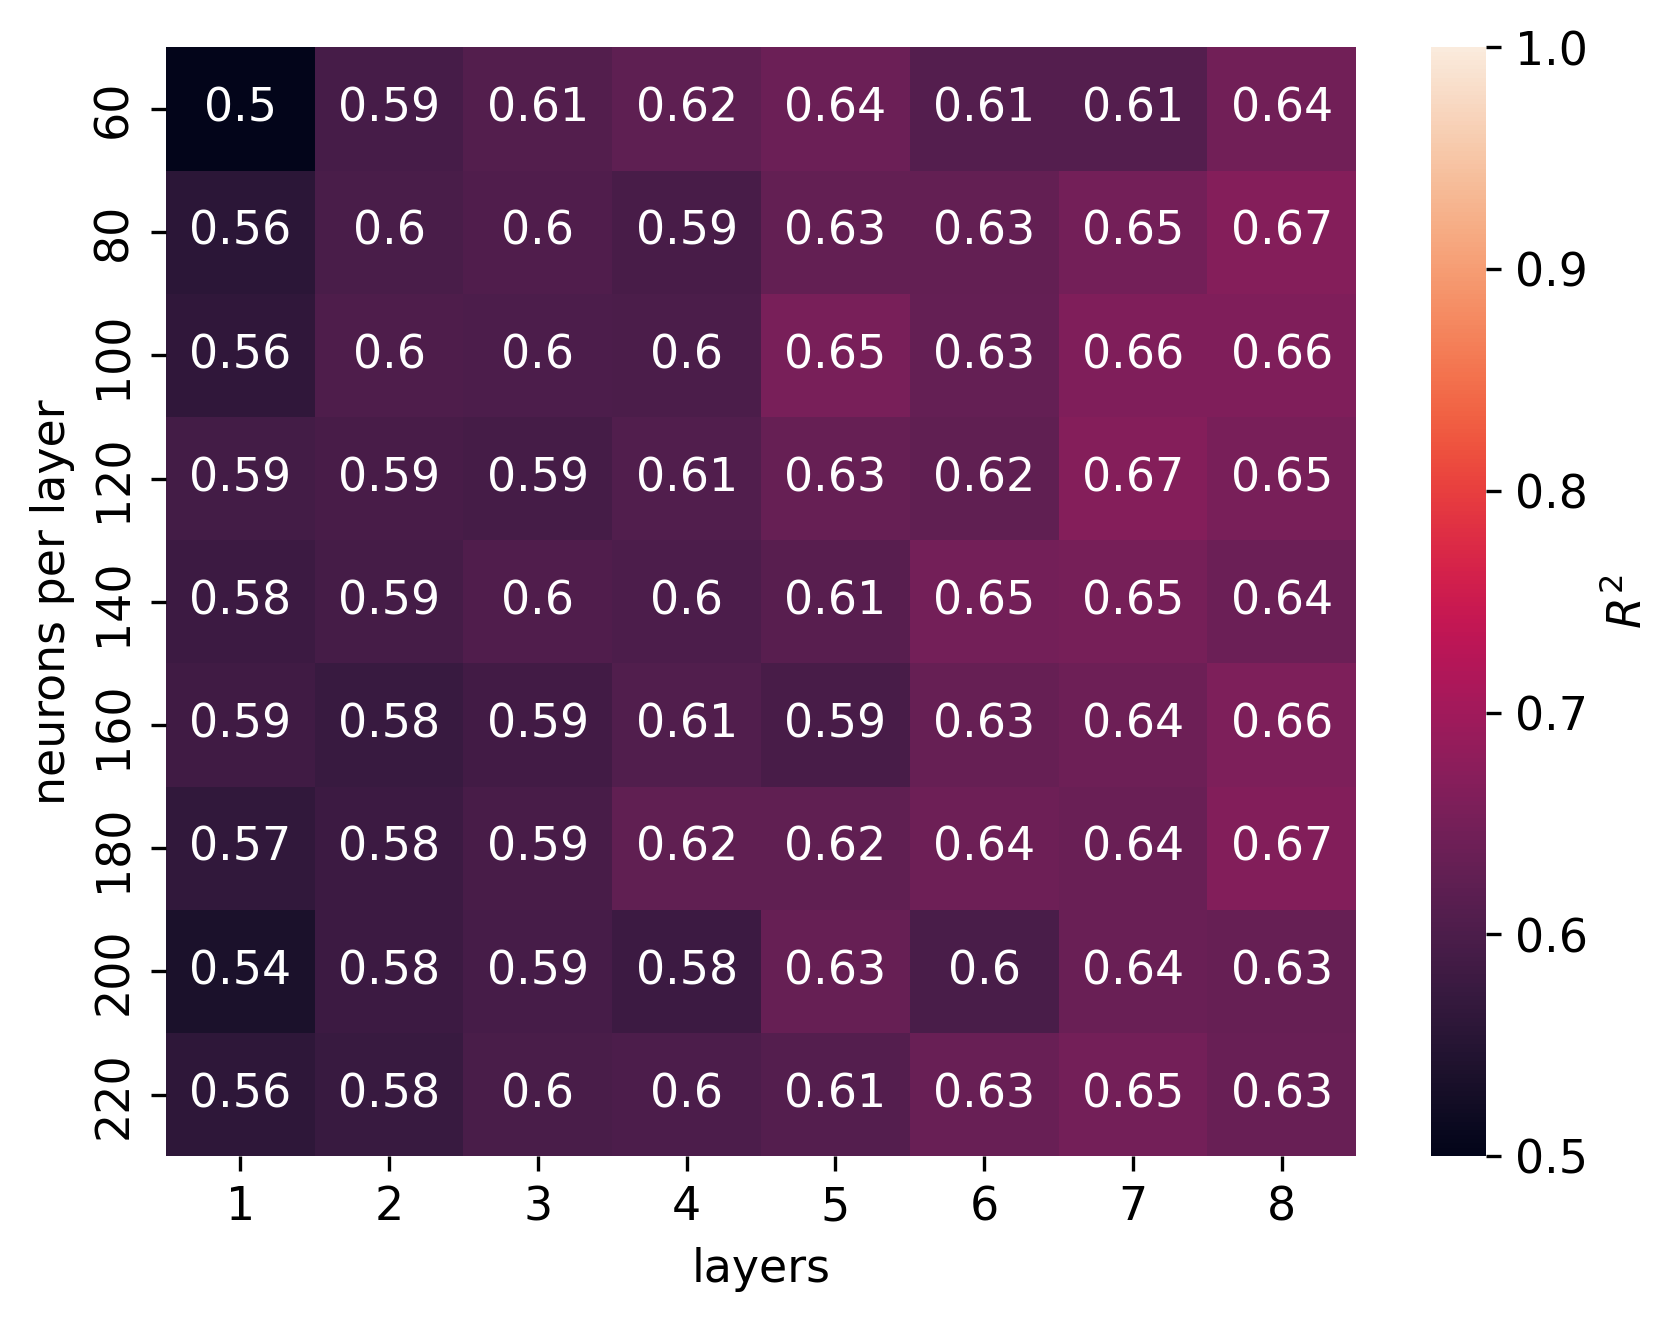
\includegraphics[width=\textwidth]{../figures/franke_L_n_test_lrelu_R2.png}
        \caption{$R^2$ for number of layers vs number of neurons}
        \label{fig:}
    \end{subfigure}
    \begin{subfigure}{.5\textwidth}
        \centering
        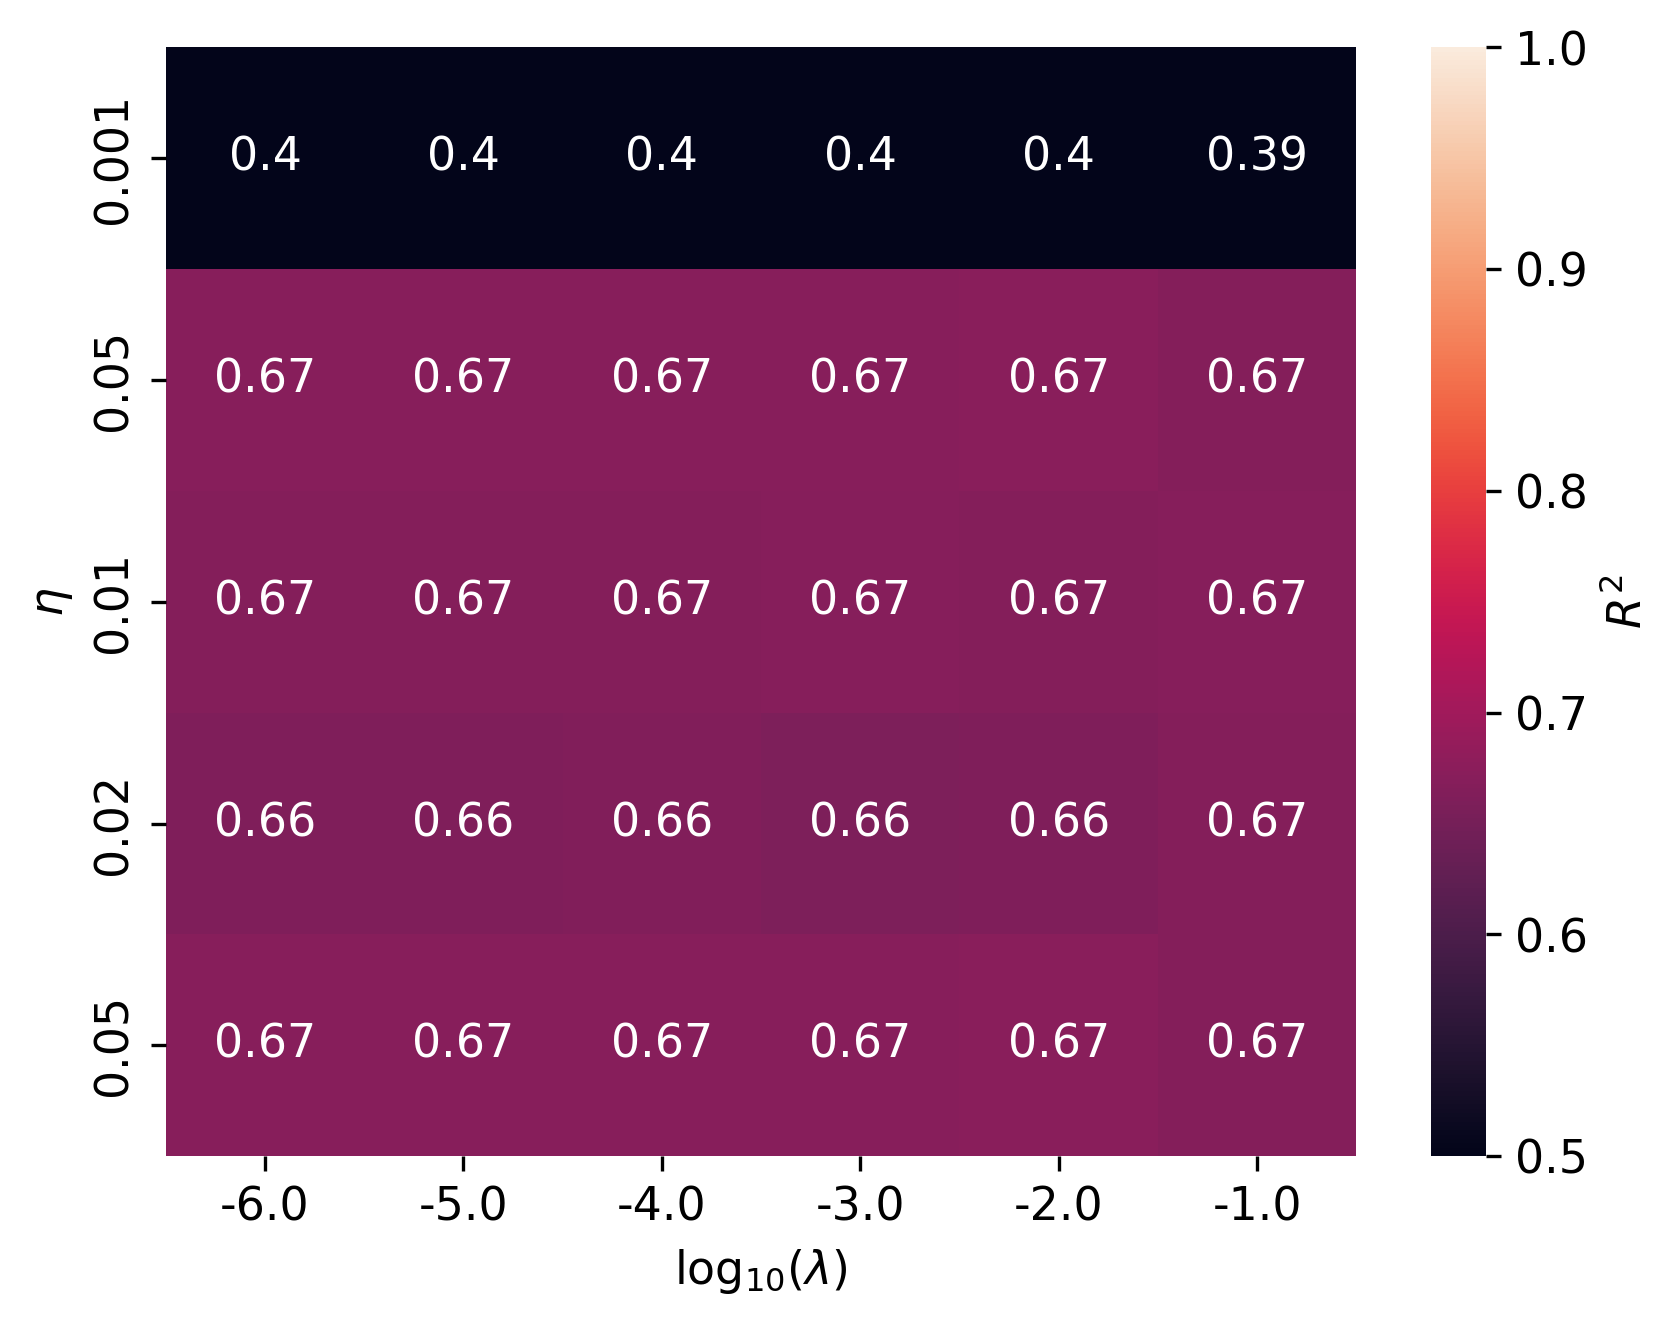
\includegraphics[width=\textwidth]{../figures/franke_eta_lmb_lrelu_R2.png}
        \caption{$R^2$ for $\eta$ vs $\lambda$}
        \label{fig:}
    \end{subfigure}
    \caption{$MSE$ and $R^2$ grid search for Franke function to find the best possible $\eta$, $\lambda$, number of layers and number of neurons for leaky ReLU as activation function}
    \label{fig:franke_grid_3}
\end{figure}
We see in figure \ref{fig:franke_grid}, \ref{fig:franke_grid_2} and \ref{fig:franke_grid_3} a $MSE$ and $R^2$ dependence on all the parameters. We end up finding the best parameters with both the highest measured $R^2$ and lowest $MSE$ as shown in table \ref{tab:franke_best}:
\begin{table}[H]
    \centering
    \caption{Lowest $MSE$ and highest $R^2$ found in grid search and the optimal parameters compared to OLS, Ridge and TensorFlow keras}
    \label{tab:franke_best}
    \begin{tabular}{|c|c|c|c|c|c|c|}
        \hline
        method                 & $MSE$  & $R^2$ & Layers & neurons & $\eta$                & $\lambda$ \\
        \hline
        \textbf{NN sigmoid}    & 0.0395 & 0.69  & 6      & 140     & 0.2                   & $10^{-5}$ \\\hline
        \textbf{NN relu}       & 0.0407 & 0.68  & 7      & 120     & 0.02                  & $10^{-2}$ \\\hline
        \textbf{NN leaky relu} & 0.0412 & 0.67  & 7      & 120     & 0.02                  & $10^{-1}$ \\\hline
        \textbf{NN relu keras} & 0.0416 & 0.68  & 3      & 100     & -                     & -         \\\hline
        \textbf{OLS}           & 0.0405 & 0.68  & -      & -       & -                     & -         \\\hline
        \textbf{Ridge}         & 0.0403 & 0.68  & -      & -       & 1.61$\times 10 ^{-7}$ & -         \\
        \hline
    \end{tabular}
\end{table}
We see in table \ref{tab:franke_best} that we manage to perform better than OLS and Ridge for each of their optimal parameters \cite{project1}. Our own neural network also outperform the neural network keras. We see each of their predictions plotted in figure \ref{fig:franke_pred} below:
\begin{figure}[H]
    \begin{subfigure}{.5\textwidth}
        \centering
        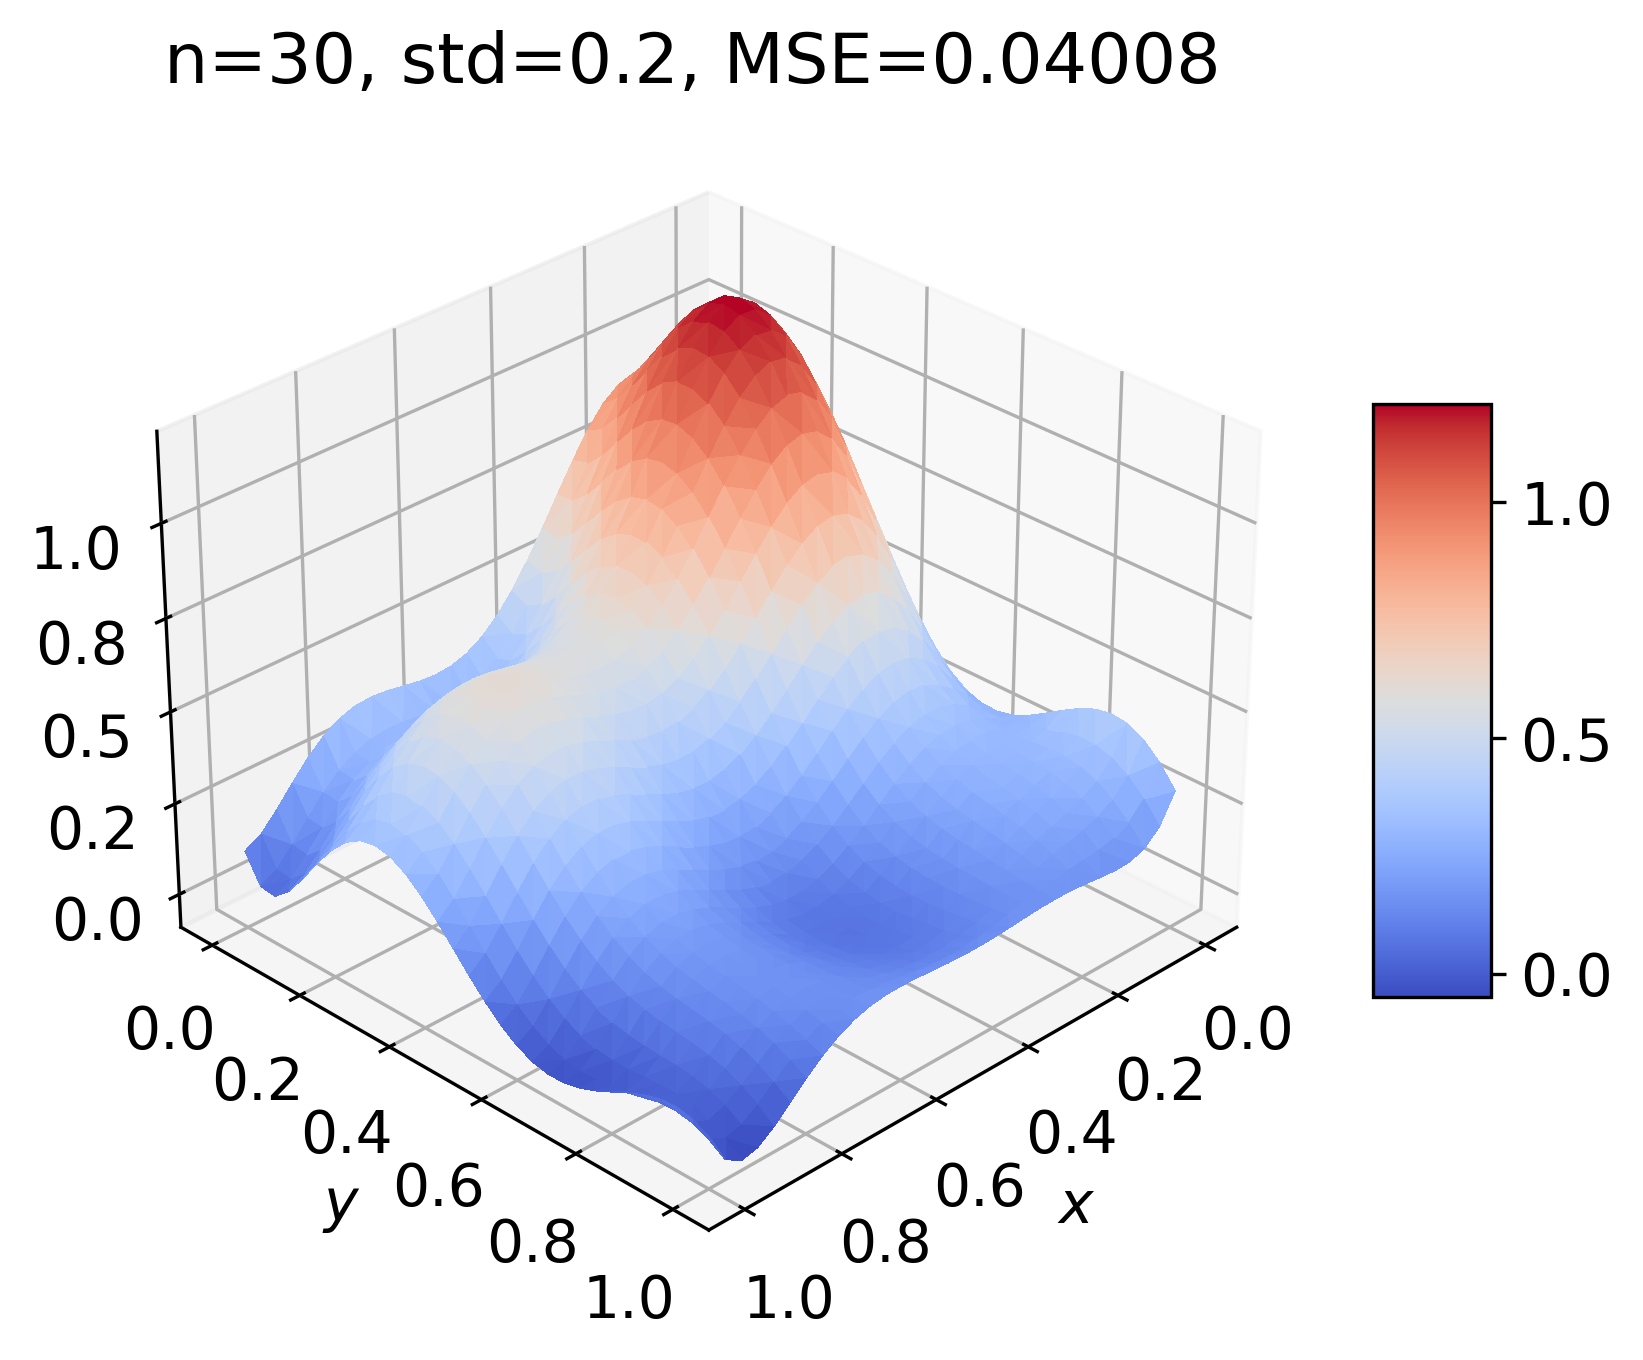
\includegraphics[width=.92\textwidth]{../figures/test_OLS.png}
        \caption{OLS}
        \label{fig:}
    \end{subfigure}
    \begin{subfigure}{.5\textwidth}
        \centering
        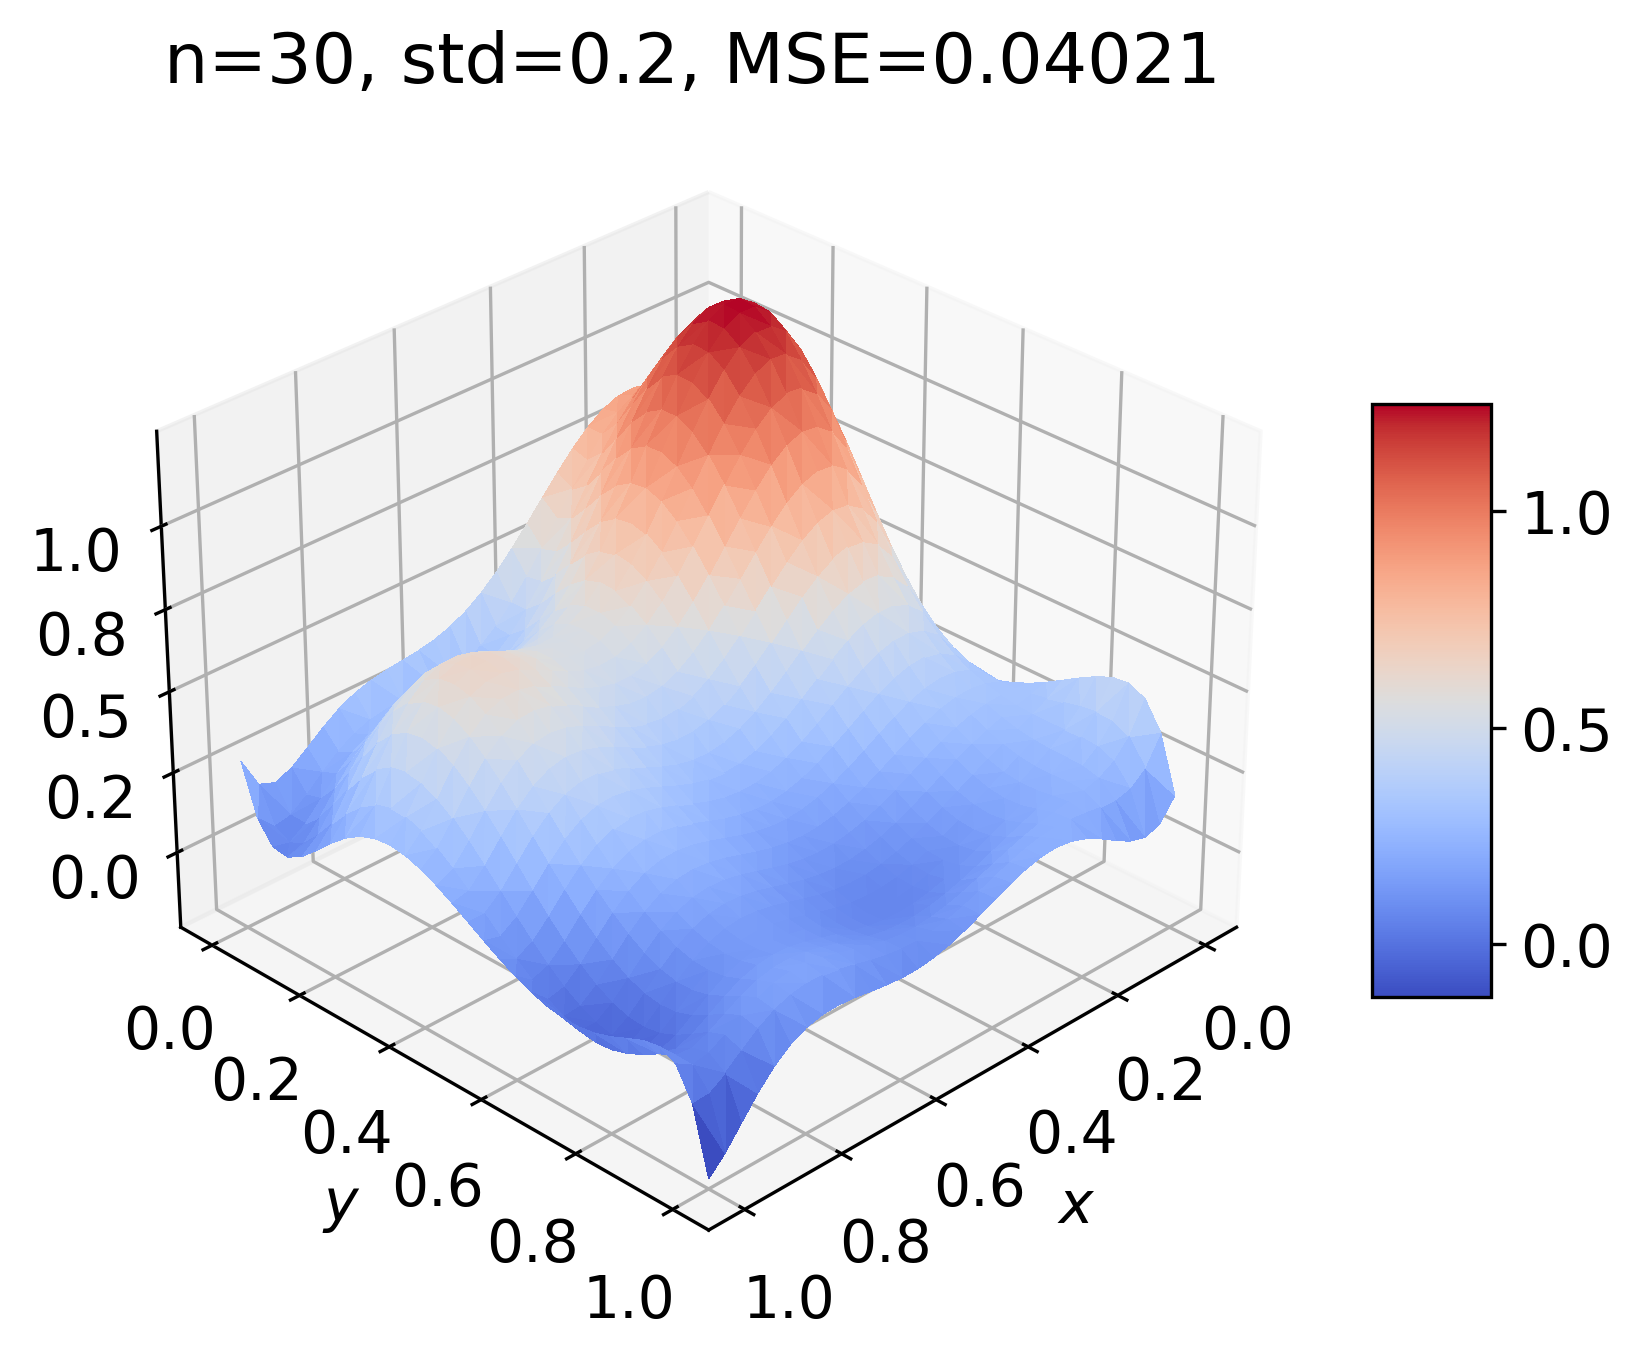
\includegraphics[width=.92\textwidth]{../figures/test_RIDGE.png}
        \caption{Ridge}
        \label{fig:}
    \end{subfigure}
    \begin{subfigure}{.5\textwidth}
        \centering
        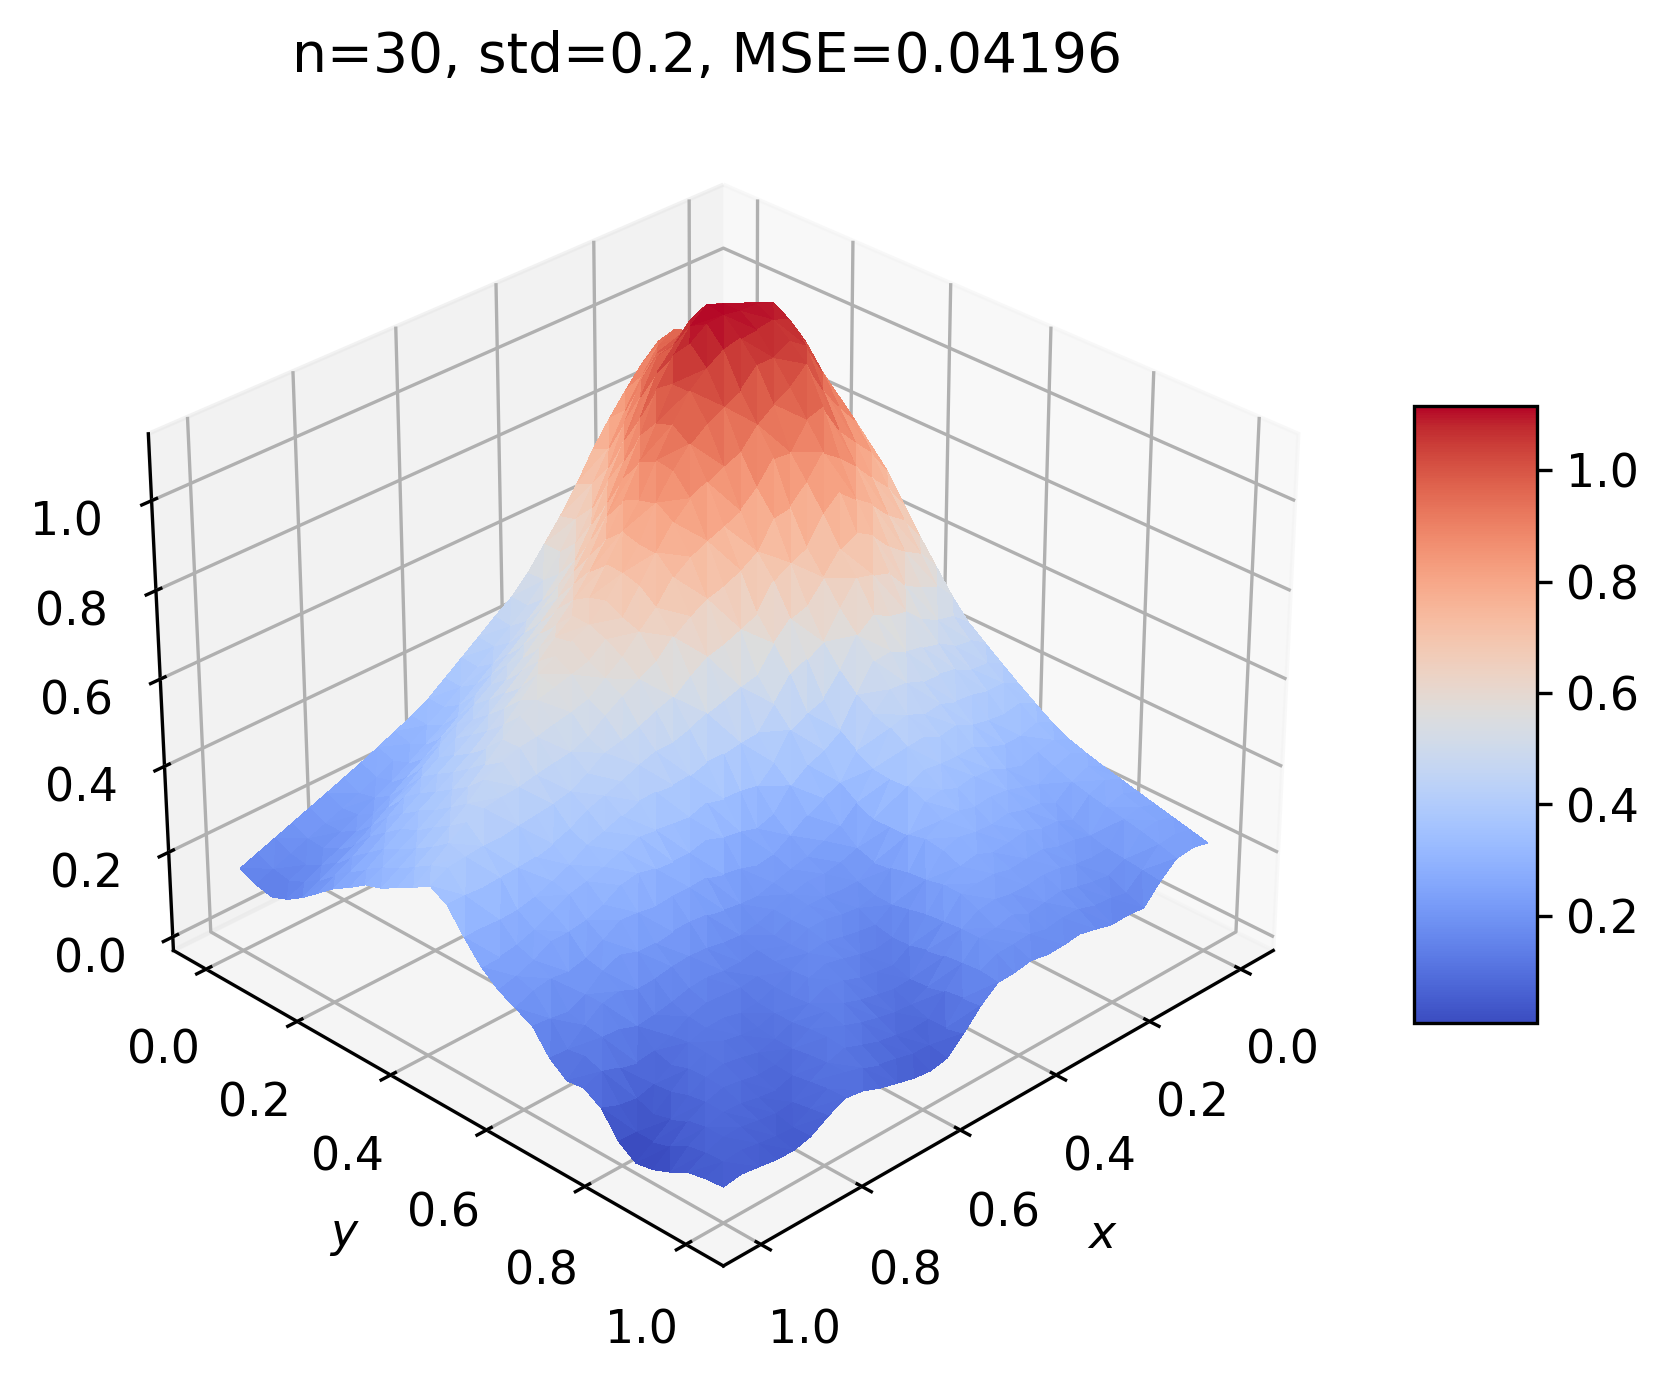
\includegraphics[width=.92\textwidth]{../figures/NN_lrelu_franke.png}
        \caption{own NN leaky ReLU}
        \label{fig:}
    \end{subfigure}
    \begin{subfigure}{.5\textwidth}
        \centering
        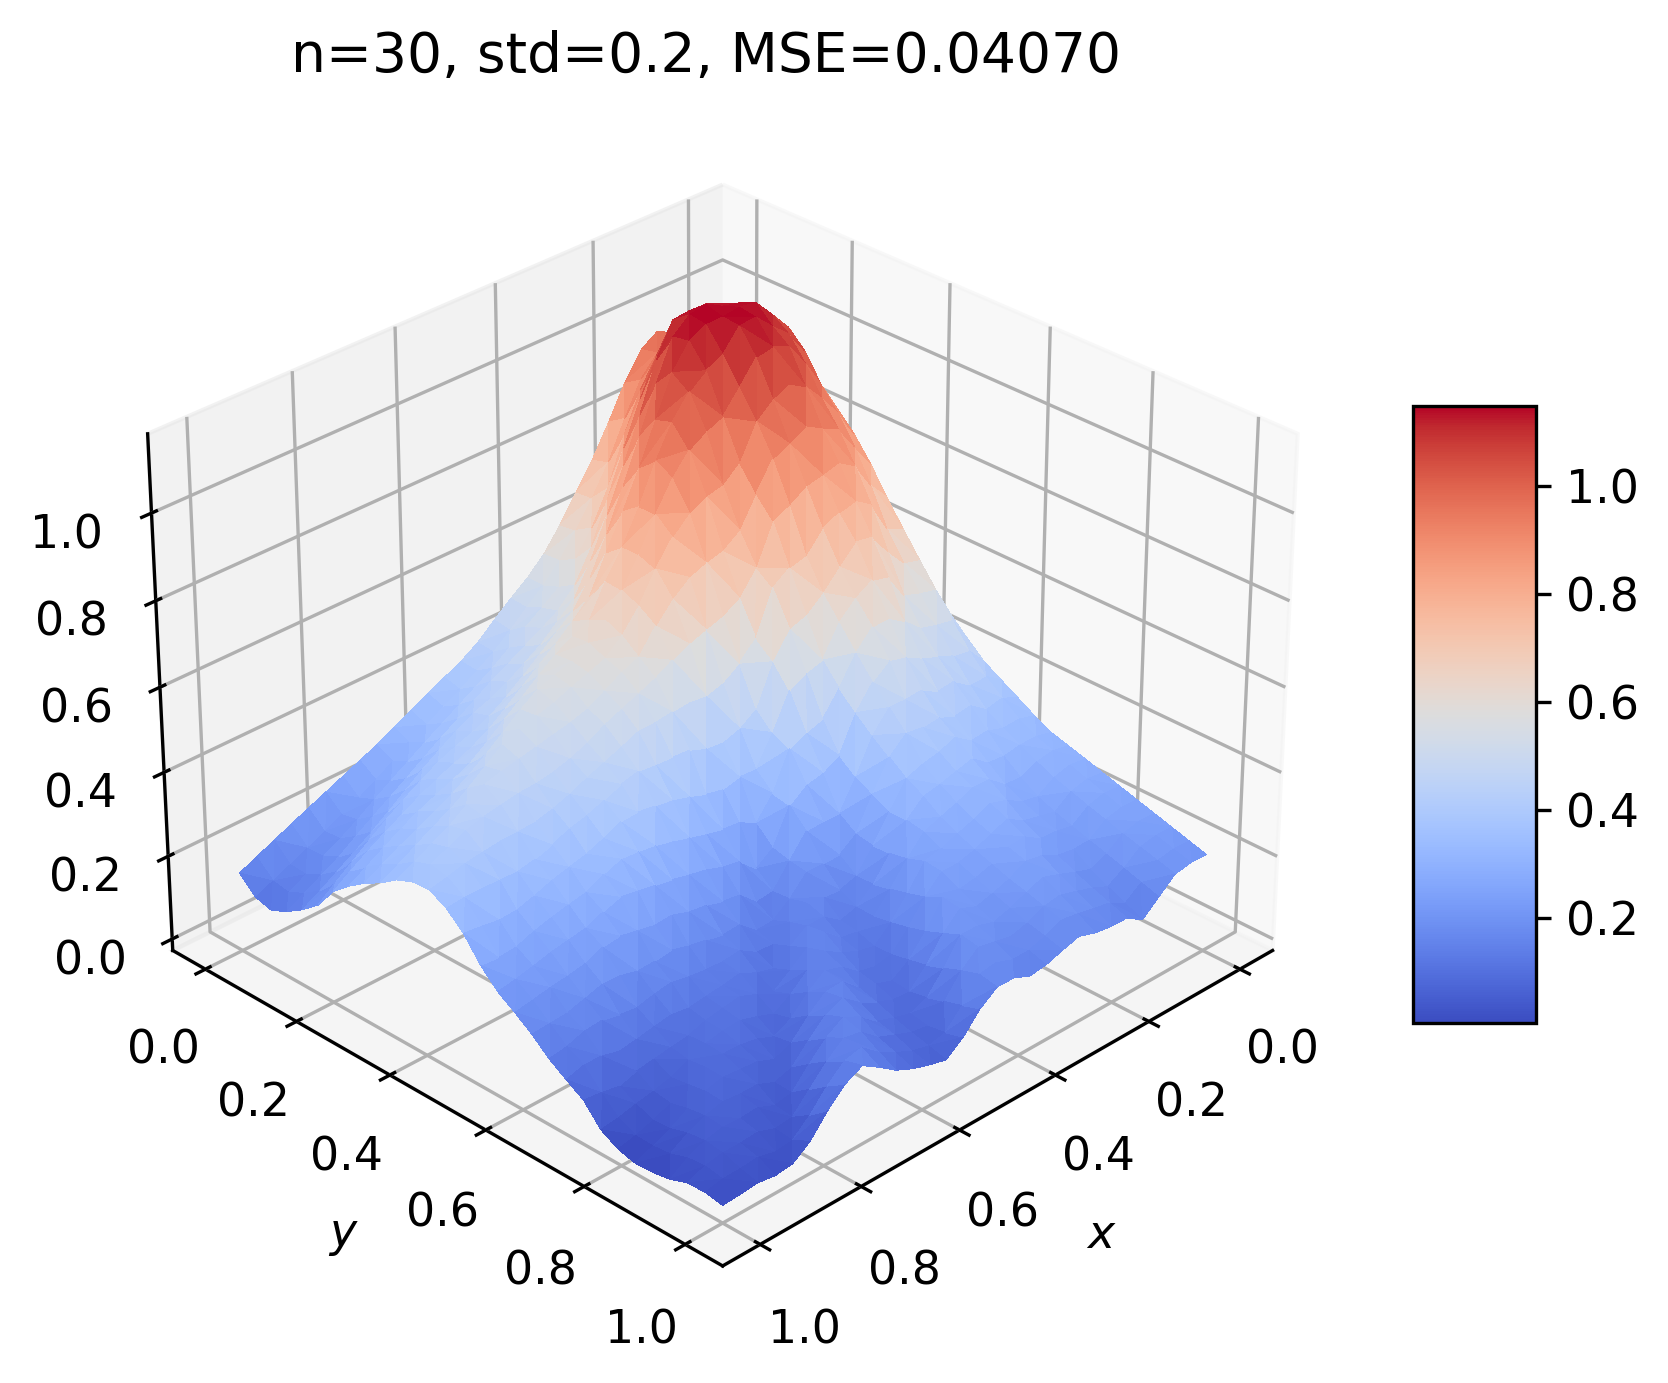
\includegraphics[width=.92\textwidth]{../figures/NN_relu_franke.png}
        \caption{own NN ReLU}
        \label{fig:}
    \end{subfigure}
    \begin{subfigure}{.5\textwidth}
        \centering
        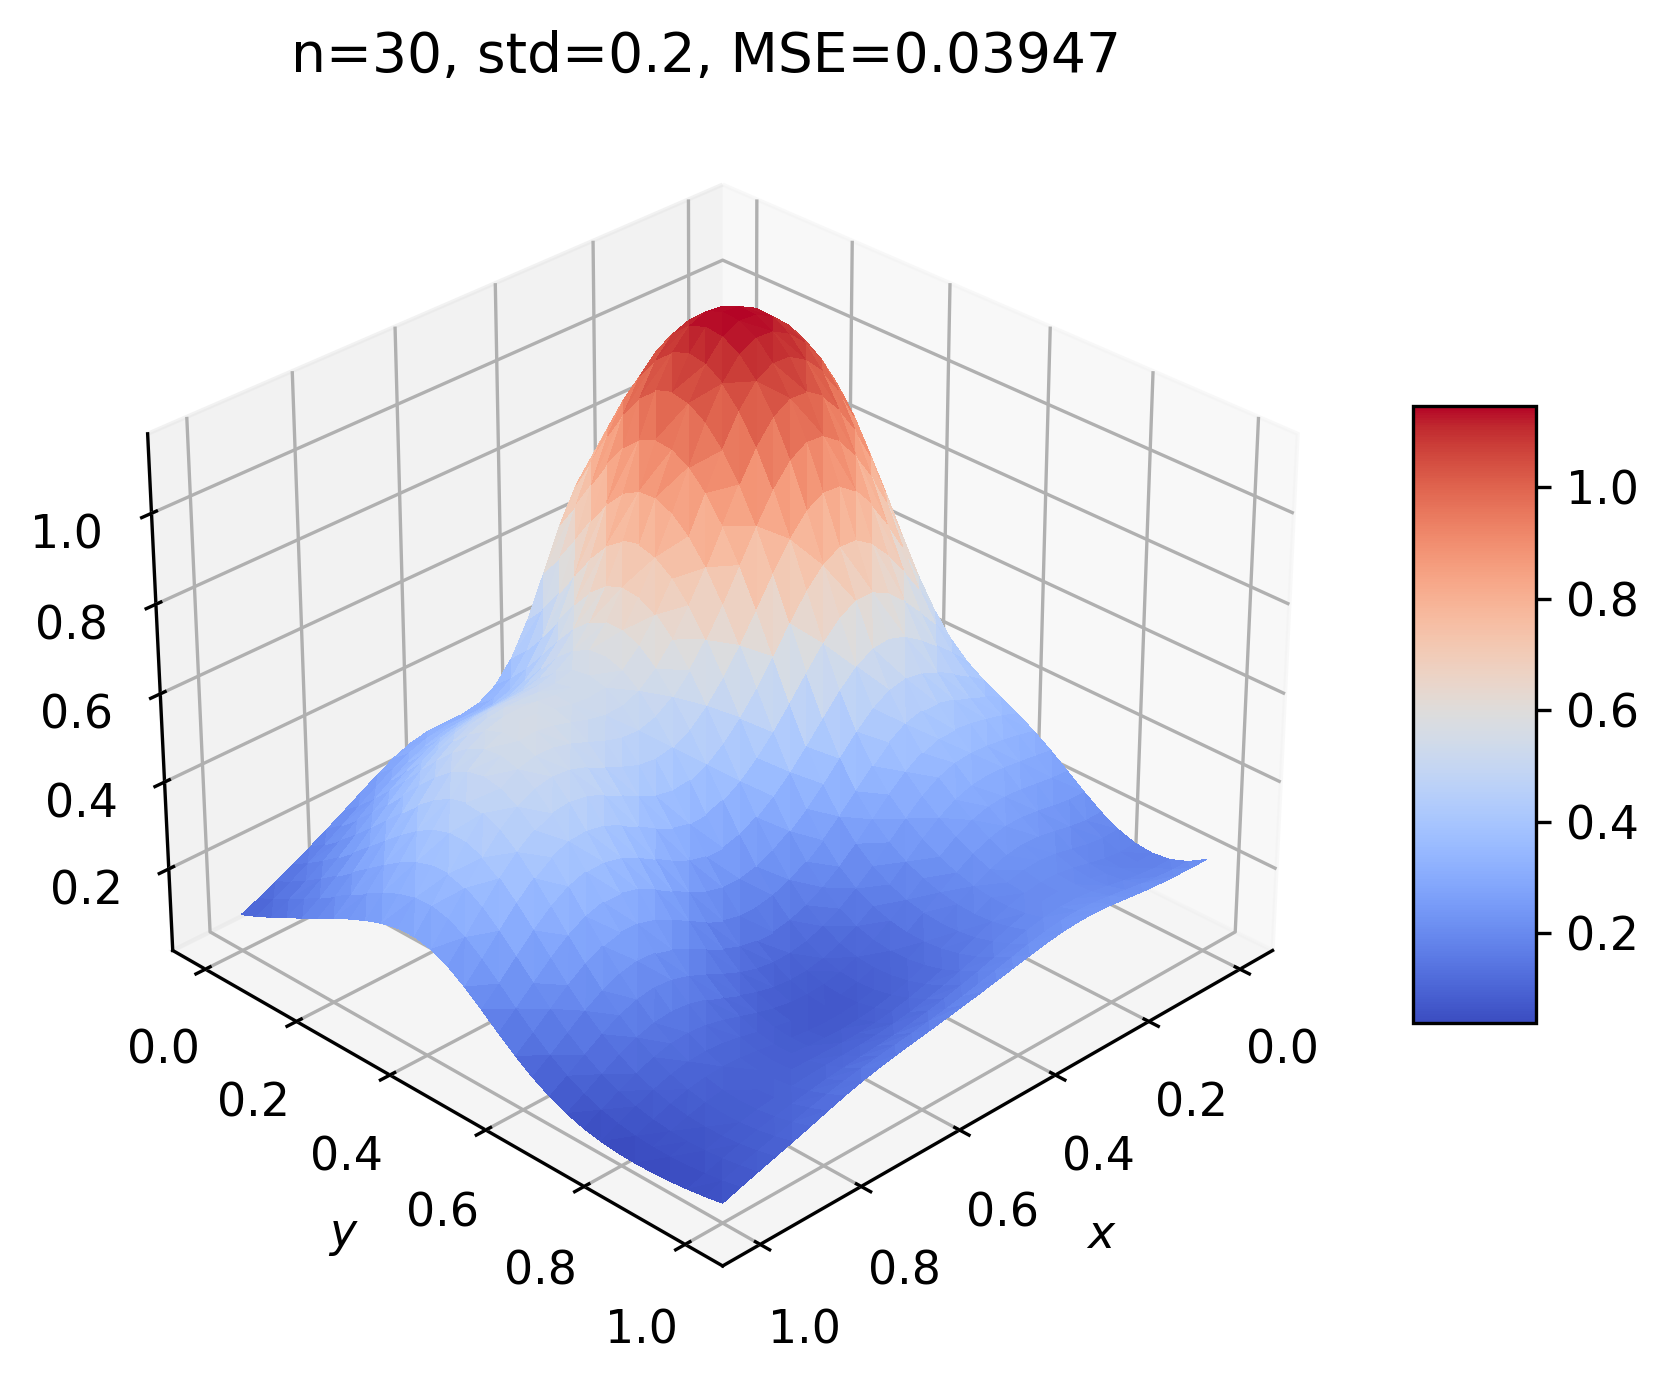
\includegraphics[width=.92\textwidth]{../figures/NN_sigmoid_franke.png}
        \caption{own NN sigmoid}
        \label{fig:}
    \end{subfigure}
    \begin{subfigure}{.5\textwidth}
        \centering
        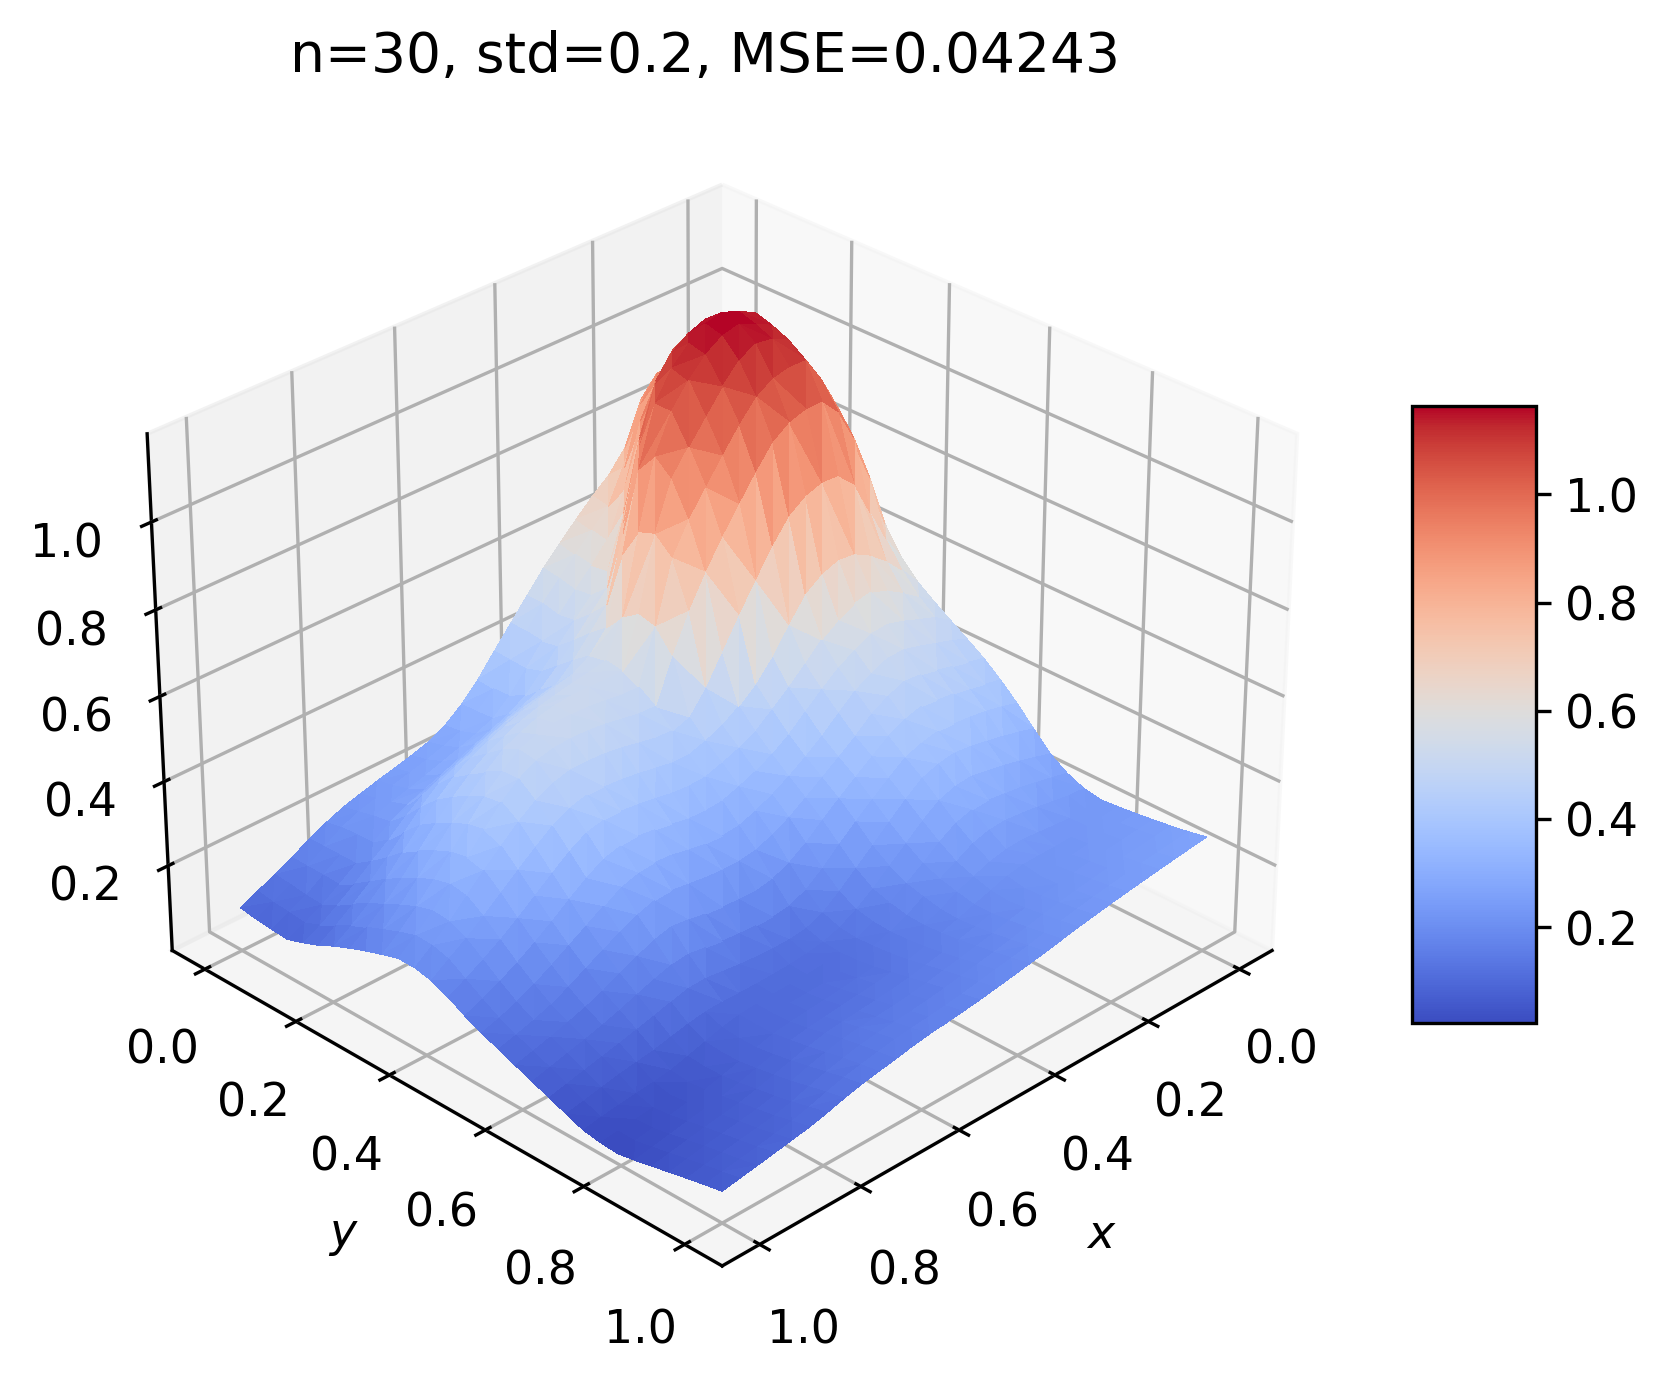
\includegraphics[width=.92\textwidth]{../figures/NN_tf_franke.png}
        \caption{NN keras}
        \label{fig:}
    \end{subfigure}
    \caption{Predictions of the Franke function using $n=30\times 30$ data points, a batch size of 60 and the optimal parameters shown in table \ref{tab:franke_best}}
    \label{fig:franke_pred}
\end{figure}

\subsection{Neural network, Logistic regression and Cancer data}
An accuracy grid search for the different gradient descent methods using logistic regression on cancer data is shown in figure \ref{fig:logreg_comp}
\begin{figure}[H]
    \begin{subfigure}{.5\textwidth}
        \centering
        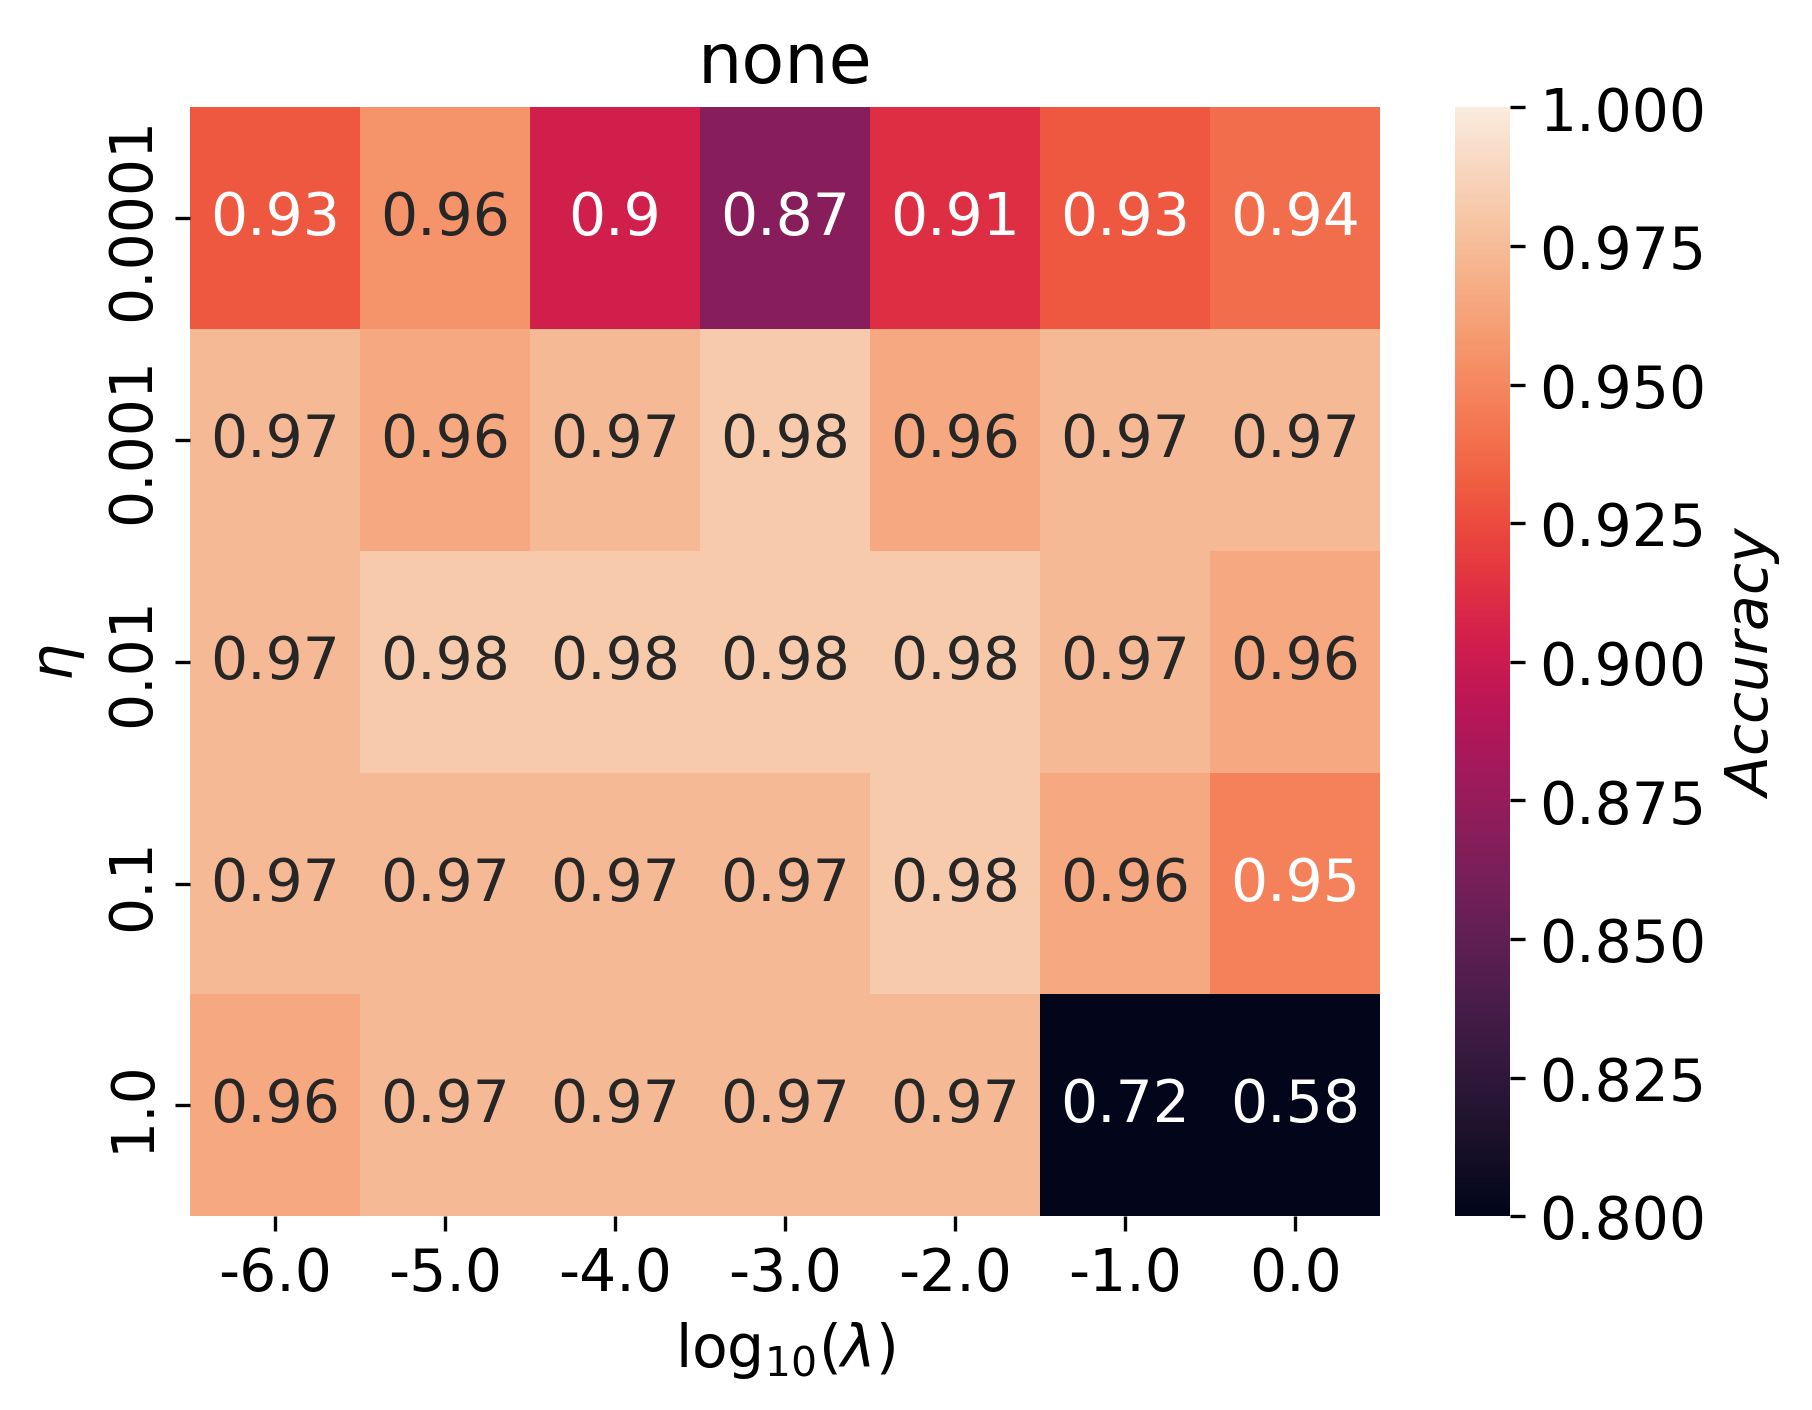
\includegraphics[width=.95\textwidth]{../figures/logreg_none.png}
        \caption{No tune}
        \label{fig:}
    \end{subfigure}
    \begin{subfigure}{.5\textwidth}
        \centering
        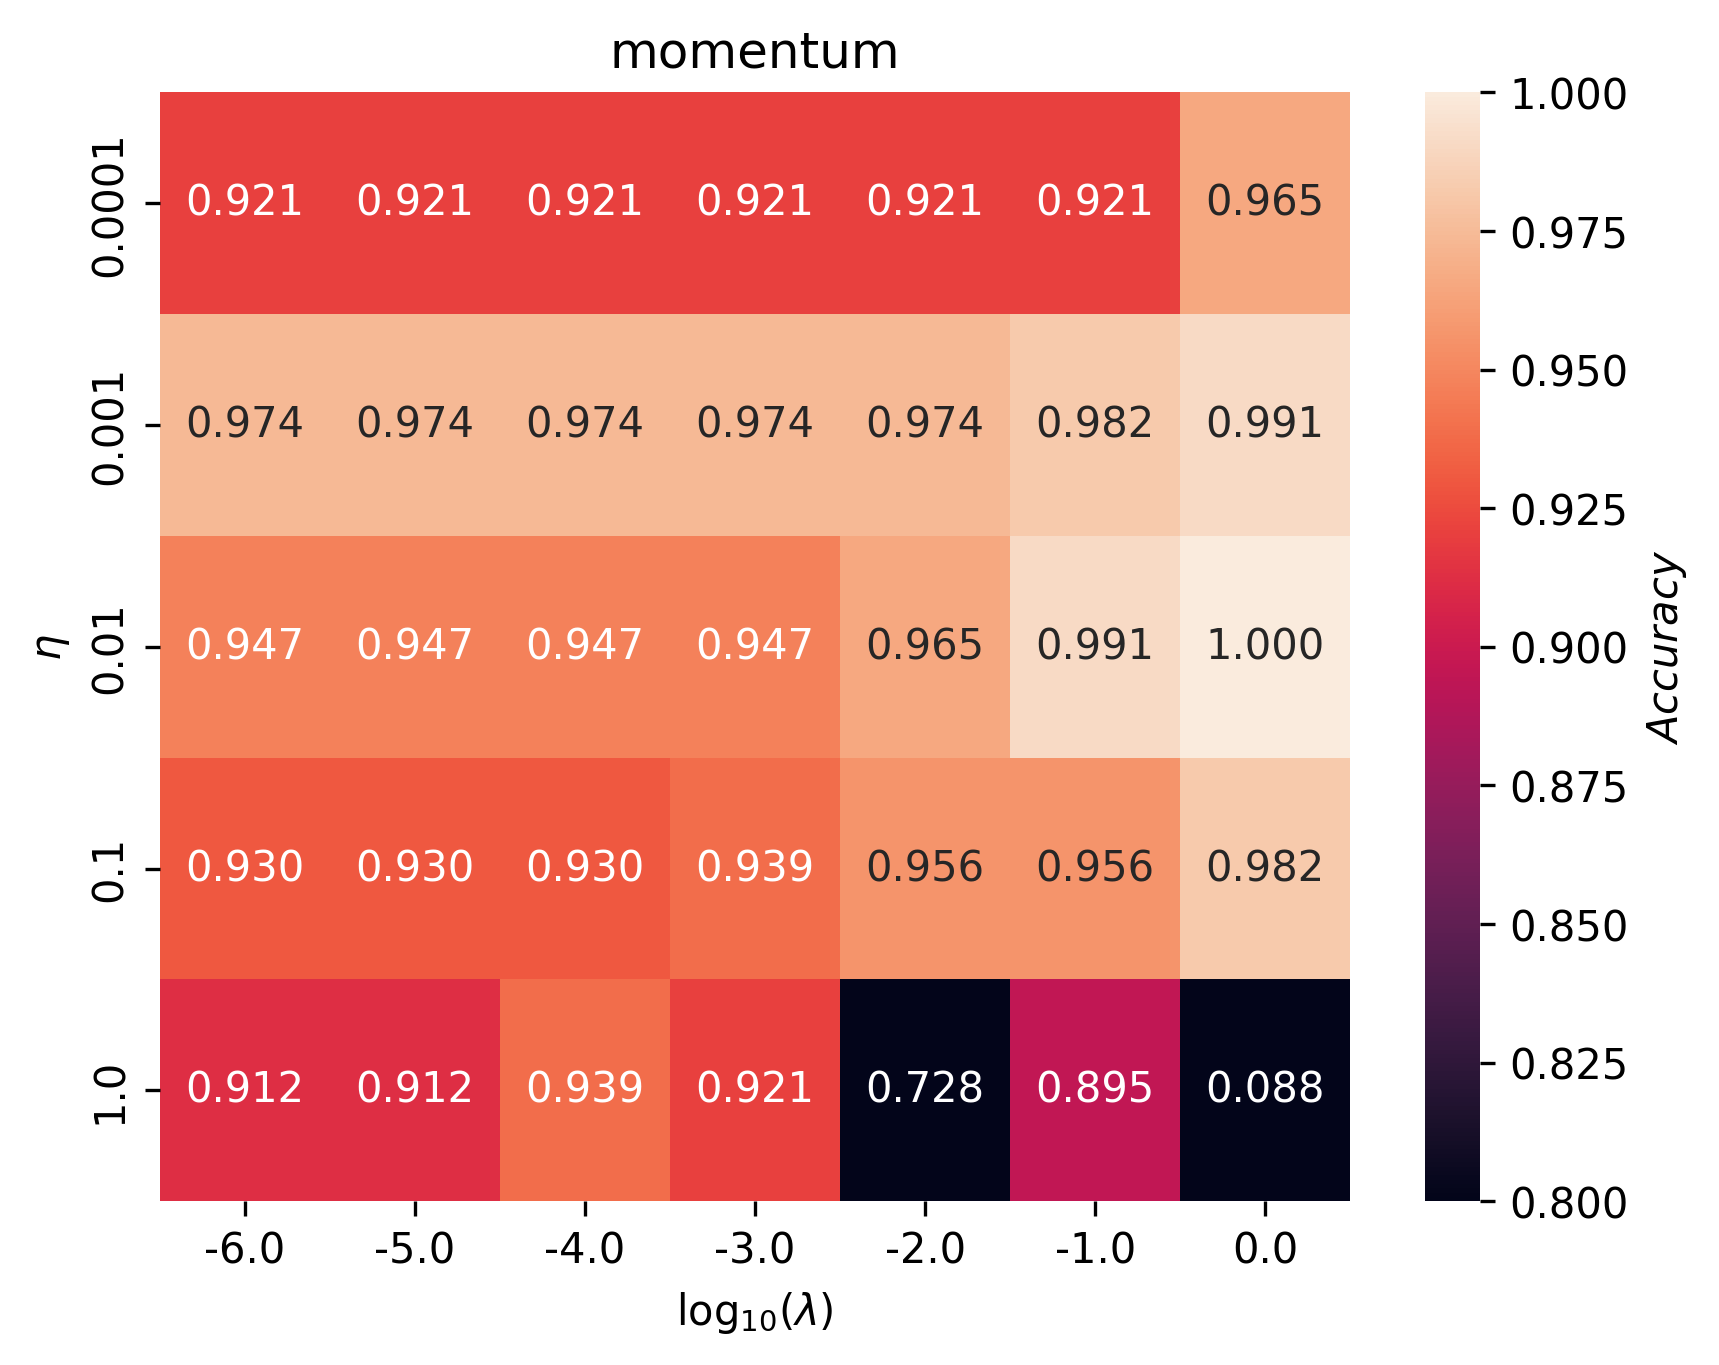
\includegraphics[width=.95\textwidth]{../figures/logreg_momentum.png}
        \caption{Momentum}
        \label{fig:}
    \end{subfigure}
    \begin{subfigure}{.5\textwidth}
        \centering
        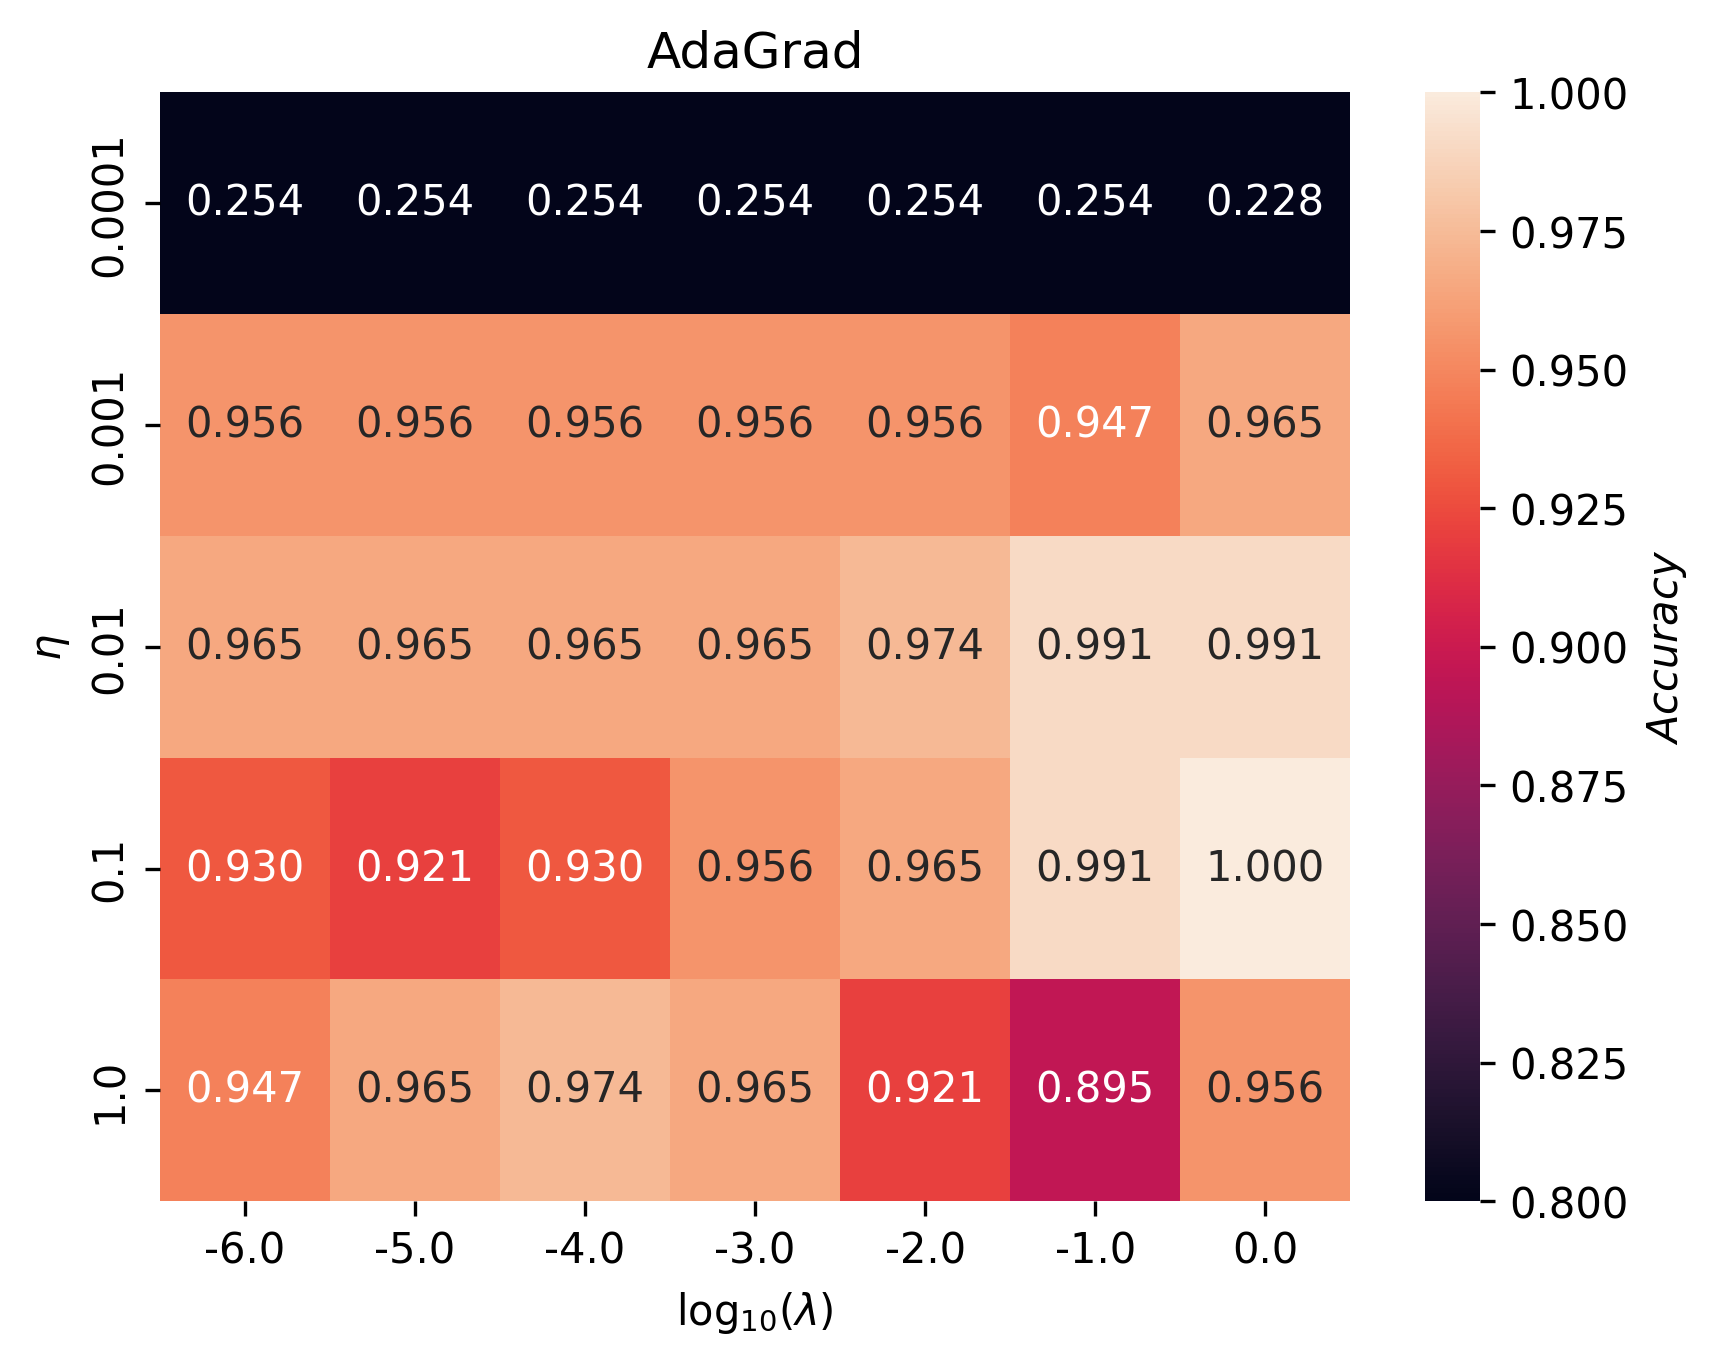
\includegraphics[width=.95\textwidth]{../figures/logreg_AdaGrad.png}
        \caption{AdaGrad}
        \label{fig:}
    \end{subfigure}
    \begin{subfigure}{.5\textwidth}
        \centering
        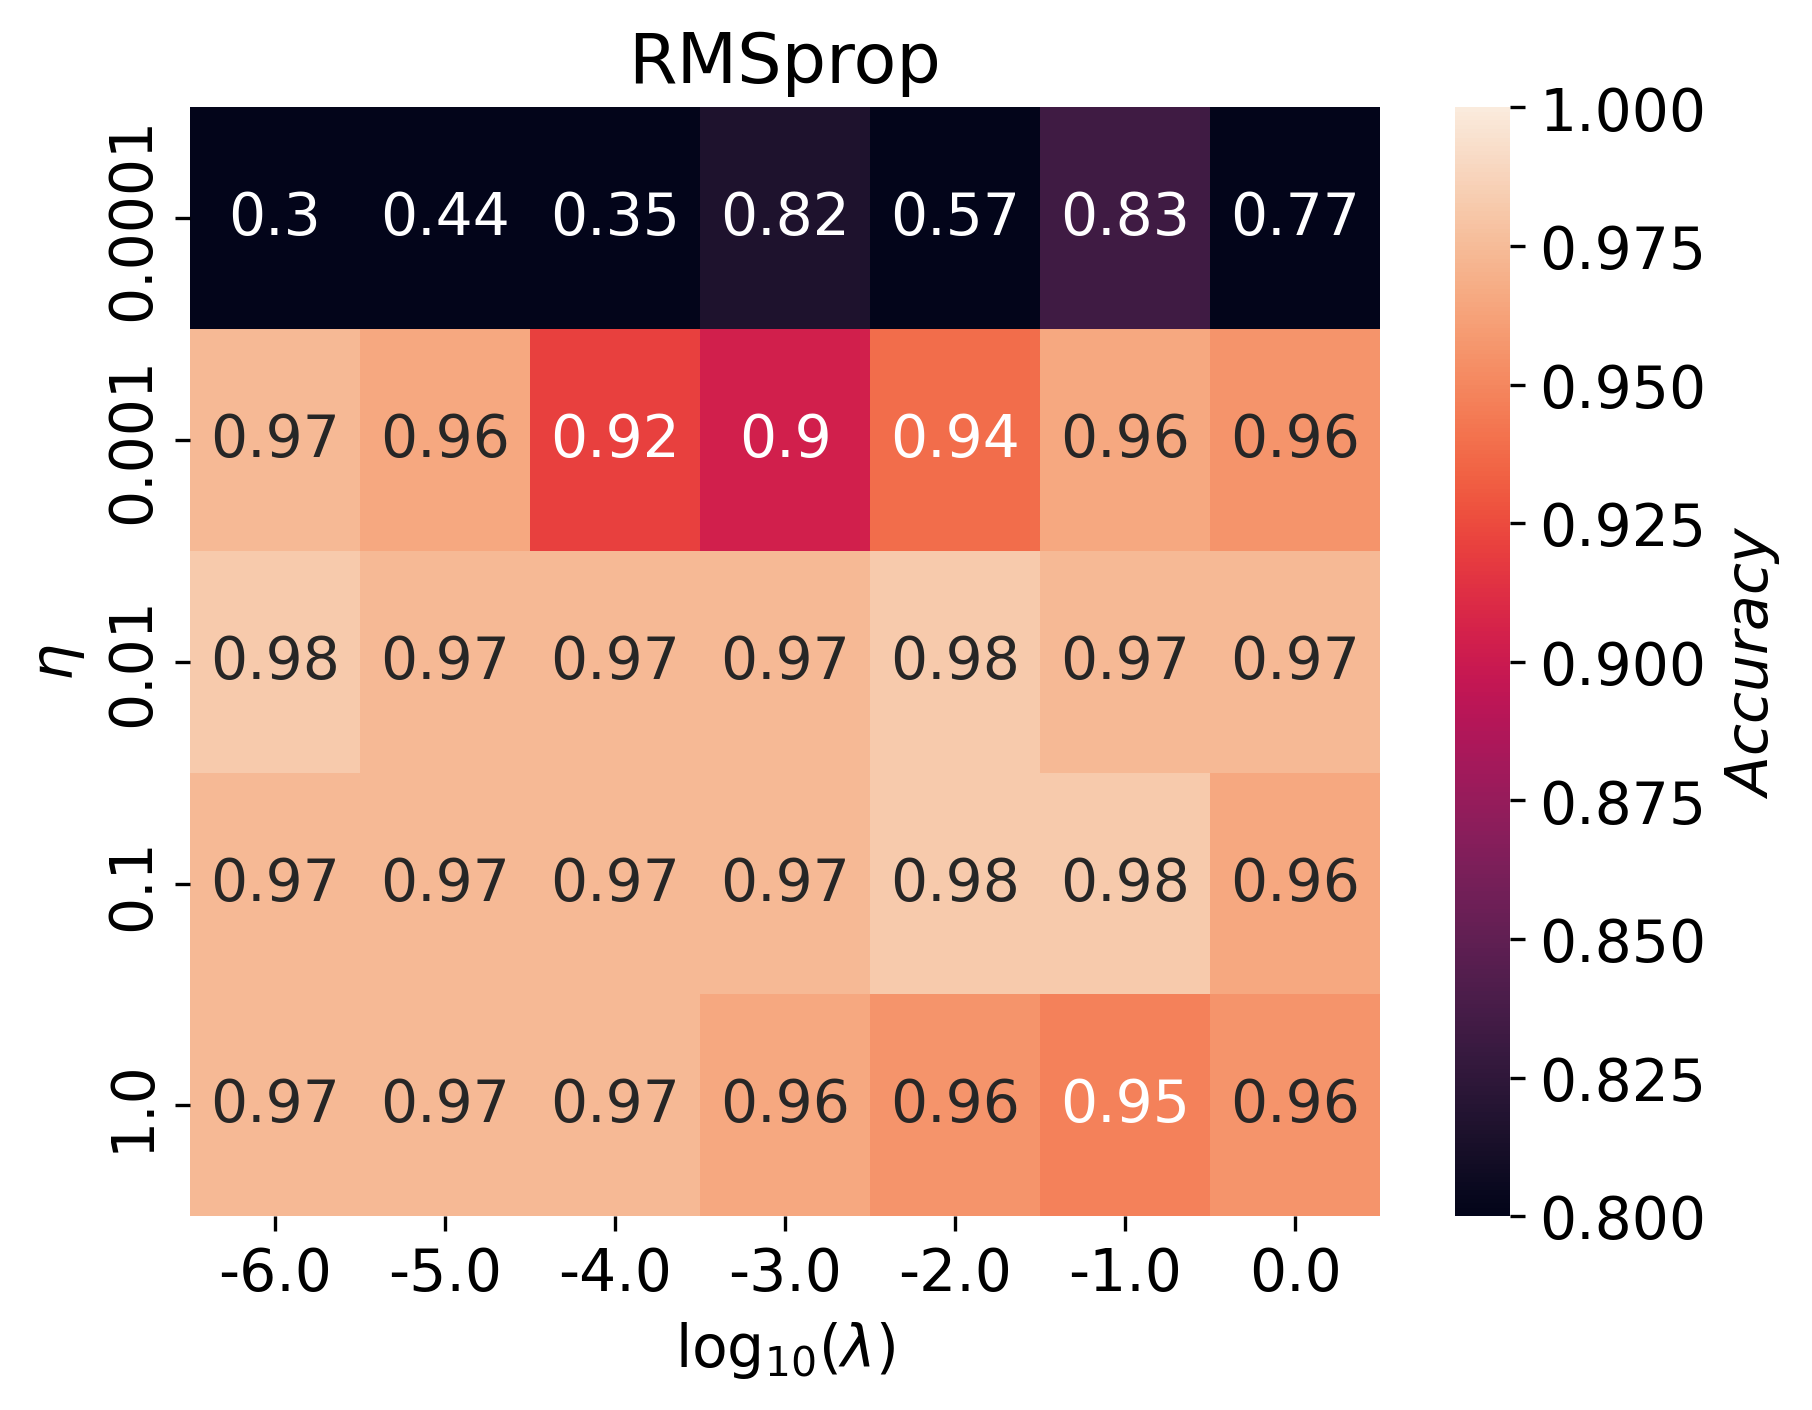
\includegraphics[width=.95\textwidth]{../figures/logreg_RMSprop.png}
        \caption{RMSprop}
        \label{fig:}
    \end{subfigure}
    \begin{subfigure}{.95\textwidth}
        \centering
        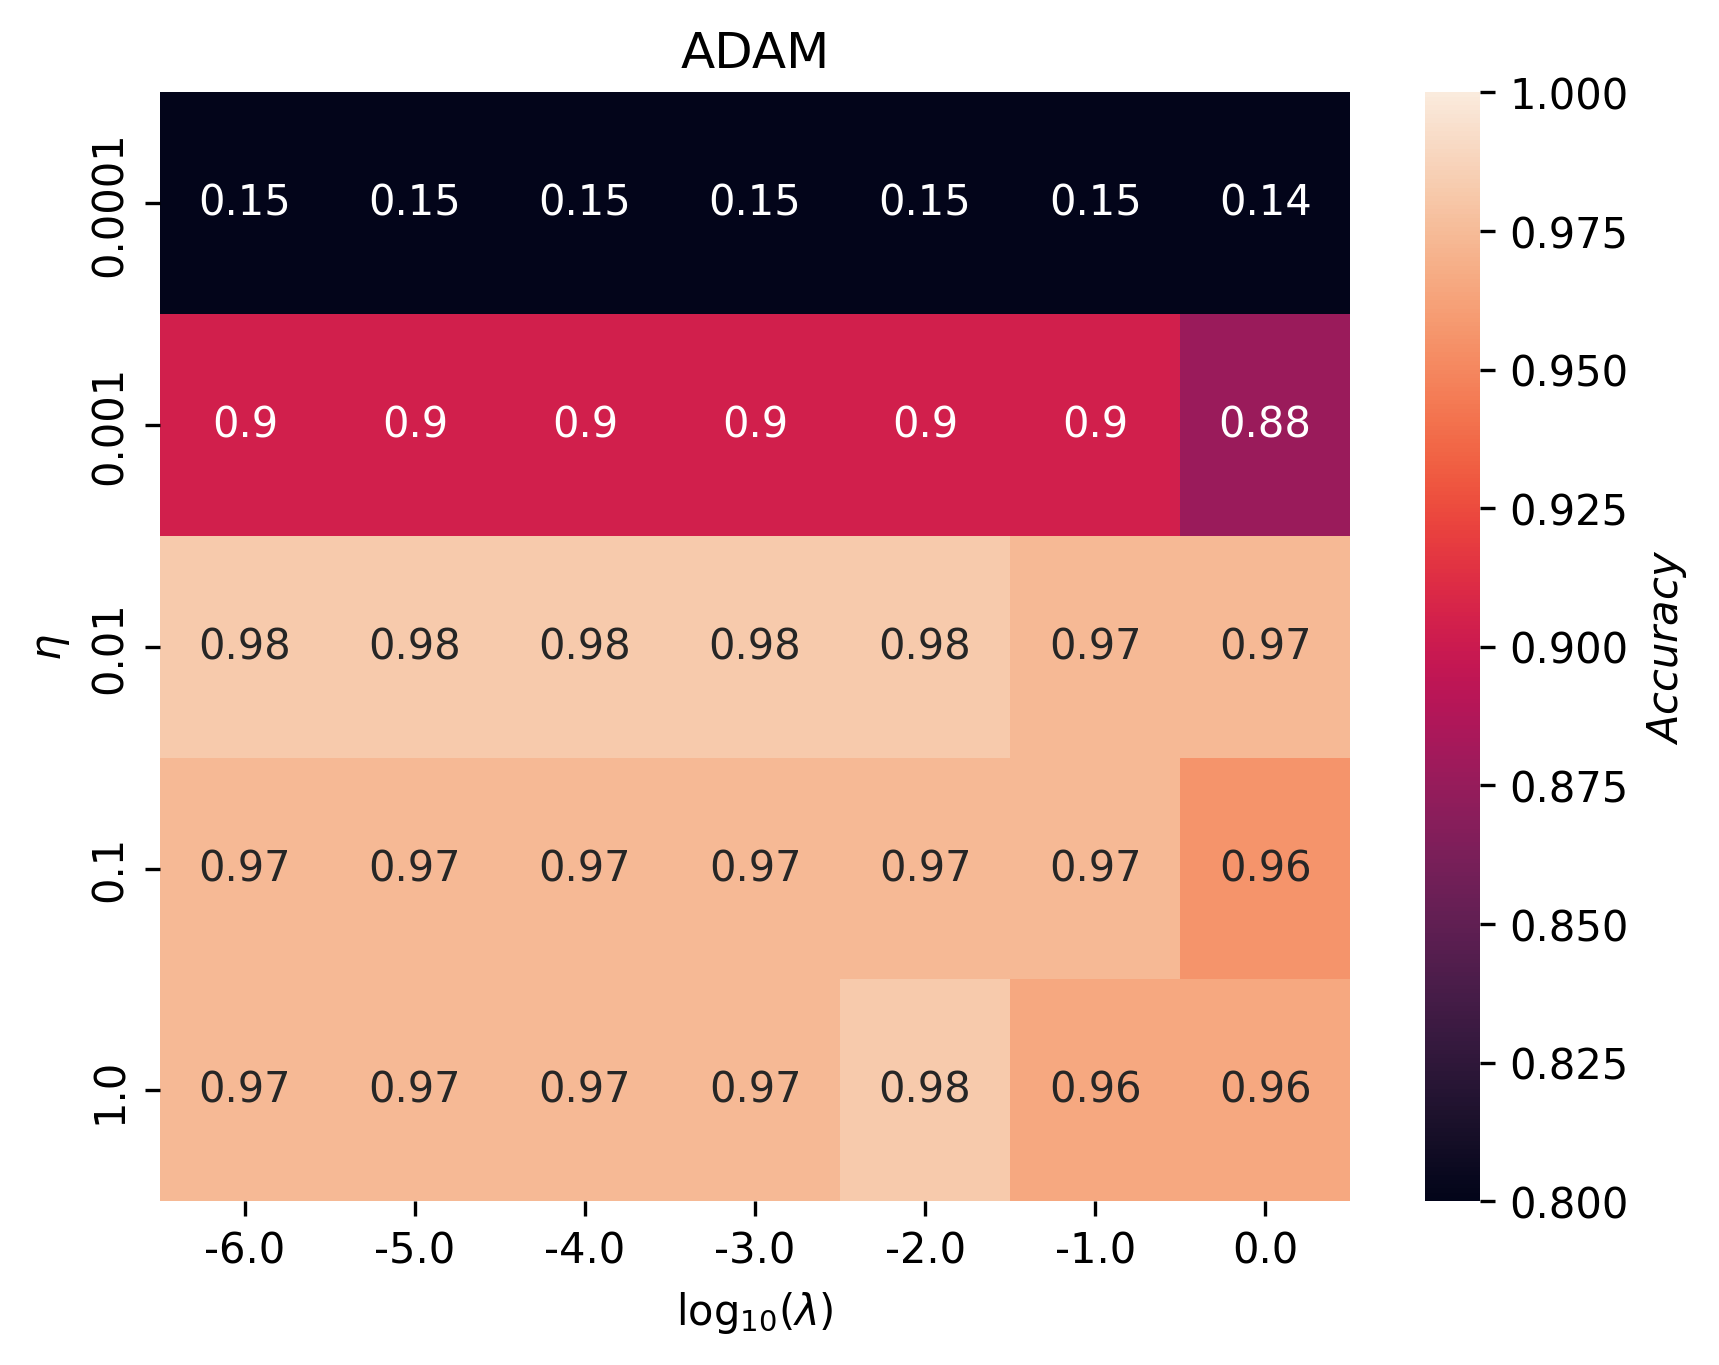
\includegraphics[width=.5\textwidth]{../figures/logreg_ADAM.png}
        \caption{ADAM}
        \label{fig:}
    \end{subfigure}
    \caption{Accuracy of logistic regression using SGD on breast cancer data for different tuning methods.}
    \label{fig:logreg_comp}
\end{figure}
In figure \ref{fig:logreg_comp} we can clearly see that logistic regression gives good results reaching an accuracy of up to 98.2\% for all tuning methods on test data.

Below in figure \ref{fig:NN_cancer} we see the accuracy of our neural network for different hyperparameters.
\begin{figure}[H]
    \begin{subfigure}{.5\textwidth}
        \centering
        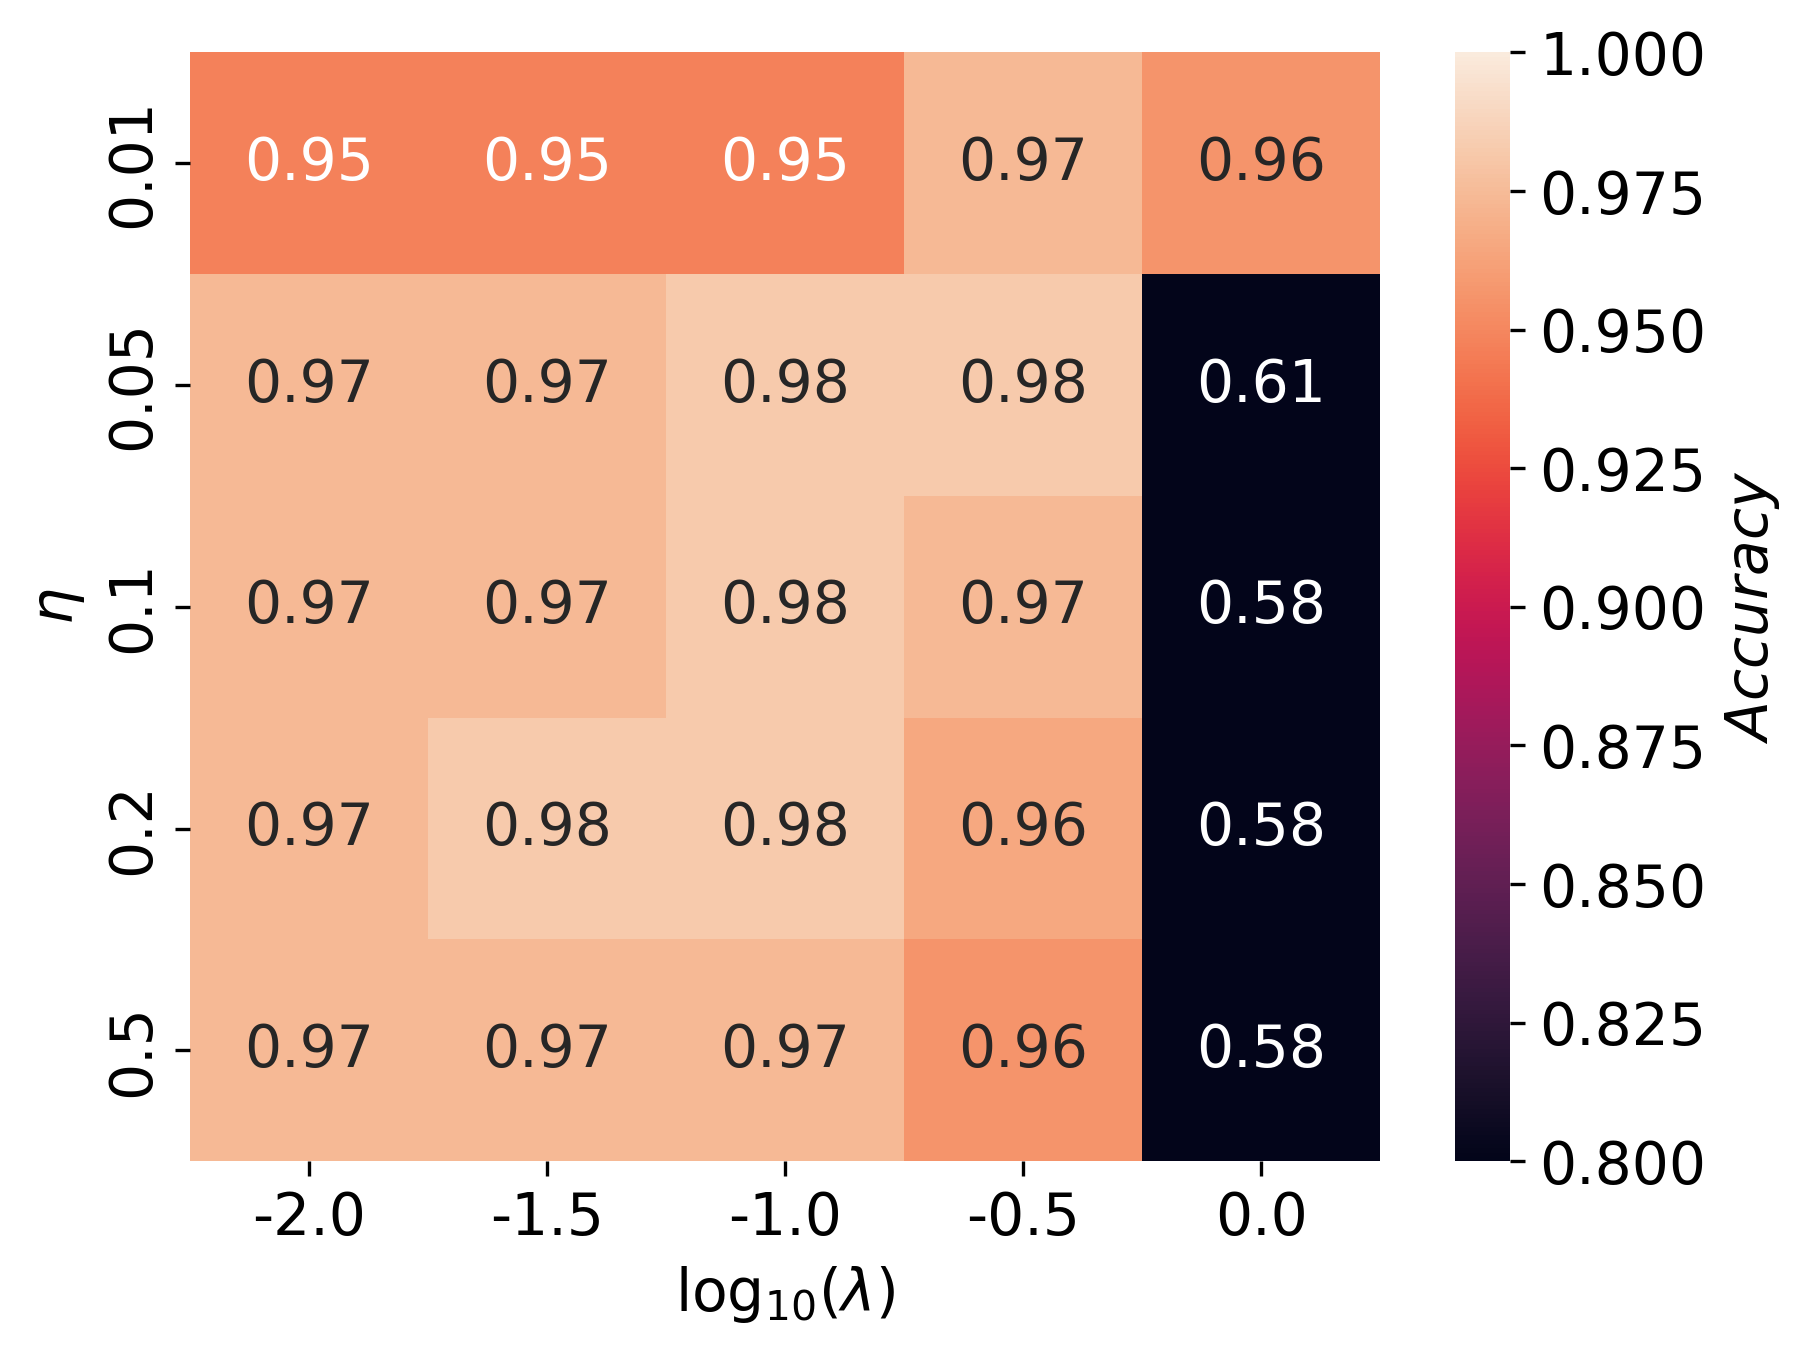
\includegraphics[width=\textwidth]{../figures/cancer_eta_lmb.png}
        \caption{}
        \label{fig:}
    \end{subfigure}
    \begin{subfigure}{.5\textwidth}
        \centering
        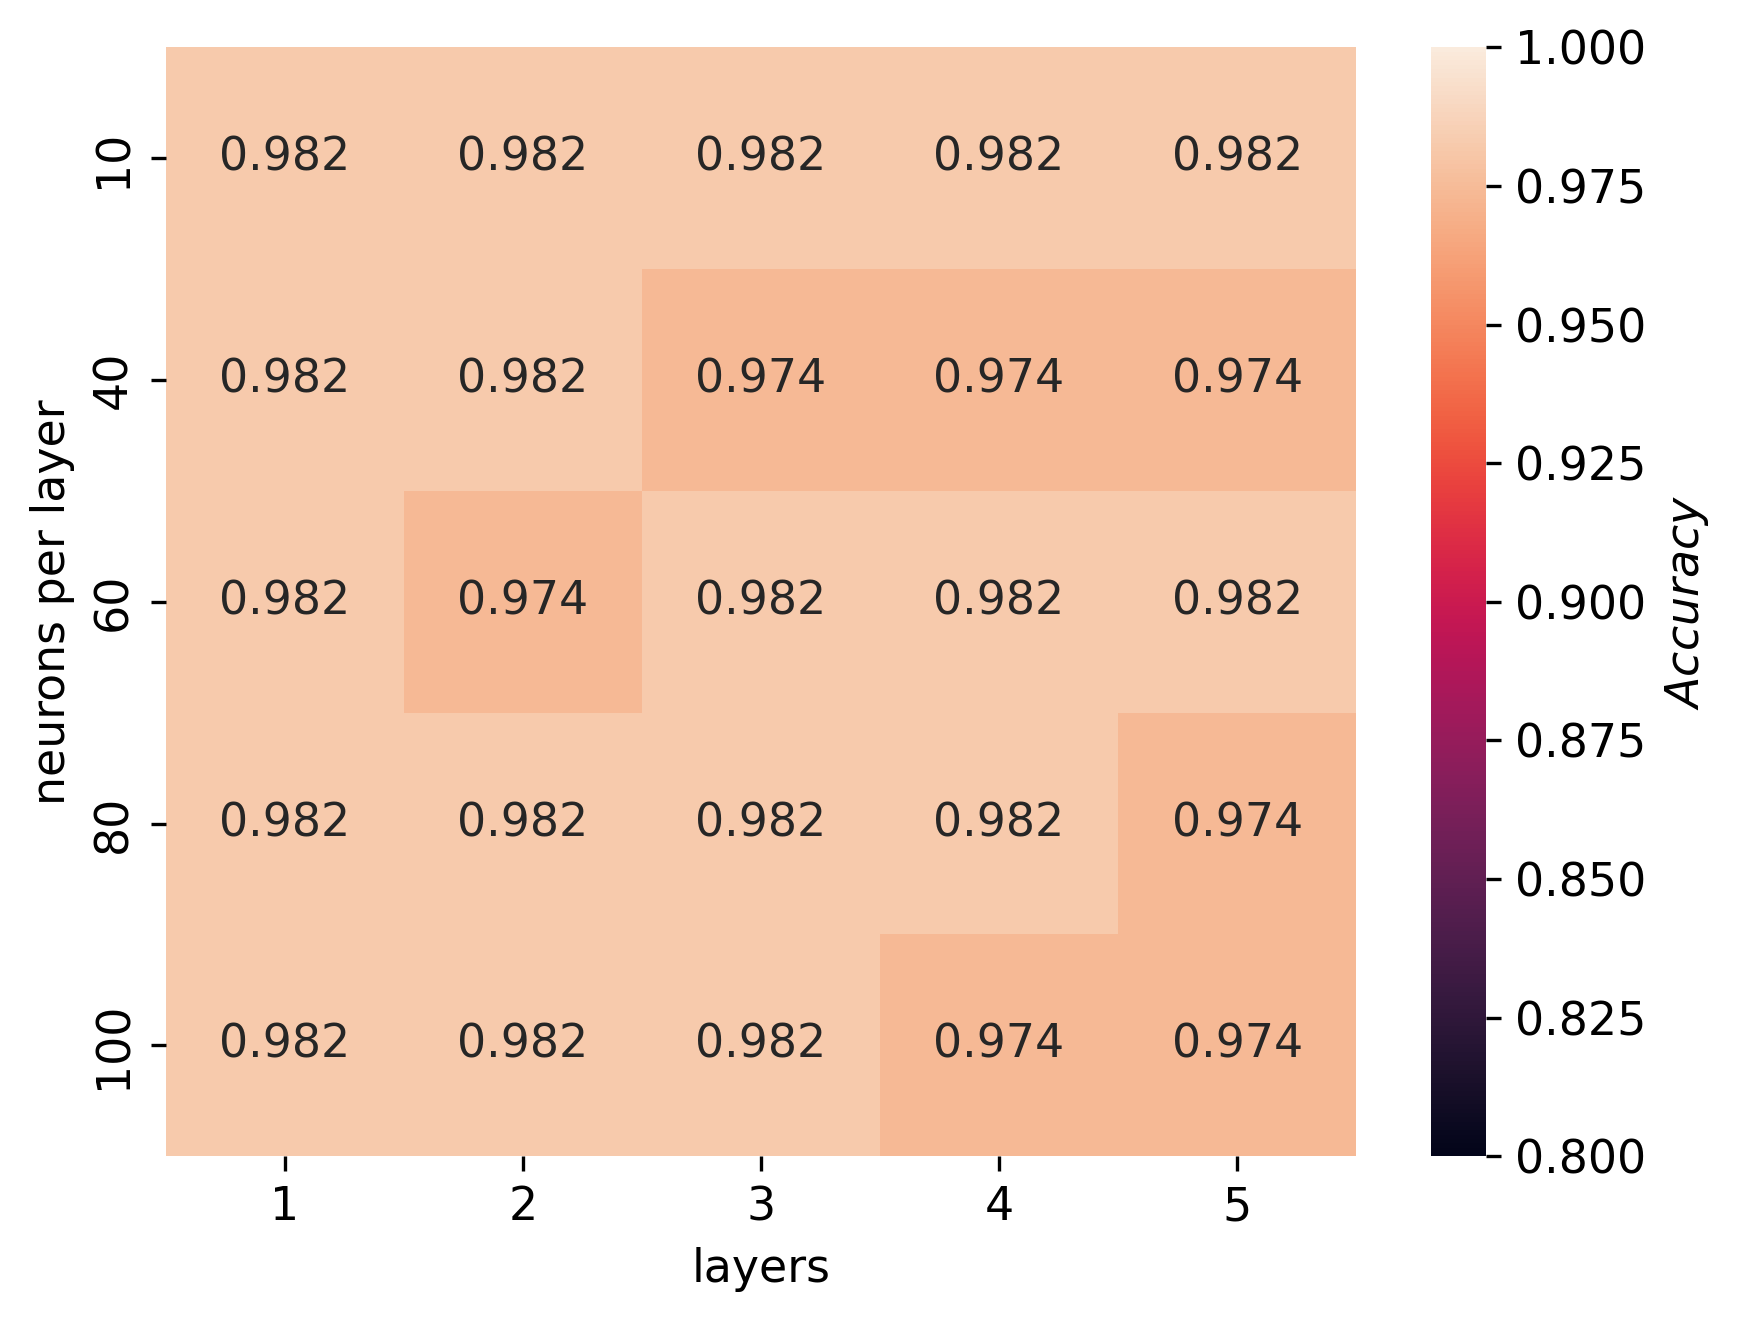
\includegraphics[width=\textwidth]{../figures/cancer_L_n_test.png}
        \caption{}
        \label{fig:}
    \end{subfigure}
    \caption{Accuracy of our own Neural Network for different choices of $\eta$, $\lambda$, number of layers, and number of neurons.}
    \label{fig:NN_cancer}
\end{figure}
We see above in figure \ref{fig:NN_cancer} similar accuracies as for logistic regression in figure \ref{fig:logreg_comp} with an accuracy hitting 98.2\%. A comparison between the two methods and scikit learns regression functionality is shown in table \ref{tab:cancer_comp}
\begin{table}[H]
    \centering
    \caption{Accuracy and optimal parameters on predicting cancer data for Neural Network and logistic regression}
    \label{tab:cancer_comp}
    \begin{tabular}{|c|c|c|c|c|c|}
        \hline
        method                   & $Accuracy$ & $\eta$ & $\lambda$ & Layers & neurons \\
        \hline
        \textbf{NN}              & 98.2\%     & 0.2    & $10^{-1}$ & 3      & 80      \\\hline
        \textbf{Logreg AdaGrad}  & 98.2\%     & 0.01   & $10^{-4}$ & -      & -       \\\hline
        \textbf{Logreg ADAM}     & 98.2\%     & 0.01   & $10^{-4}$ & -      & -       \\\hline
        \textbf{Logreg RMSprop}  & 98.2\%     & 0.01   & $10^{-4}$ & -      & -       \\\hline
        \textbf{Logreg Momentum} & 98.2\%     & 0.01   & $10^{-2}$ & -      & -       \\\hline
        \textbf{Logreg no tune}  & 98.2\%     & 0.01   & $10^{-4}$ & -      & -       \\\hline
        \textbf{Logreg scikit}   & 97.4\%     & -      & -         & -      & -       \\\hline
    \end{tabular}
\end{table}

Using another seed for our train-test split and shuffle we get the following results in figure \ref{fig:cancer_best}
\begin{figure}[H]
    \begin{subfigure}{.5\textwidth}
        \centering
        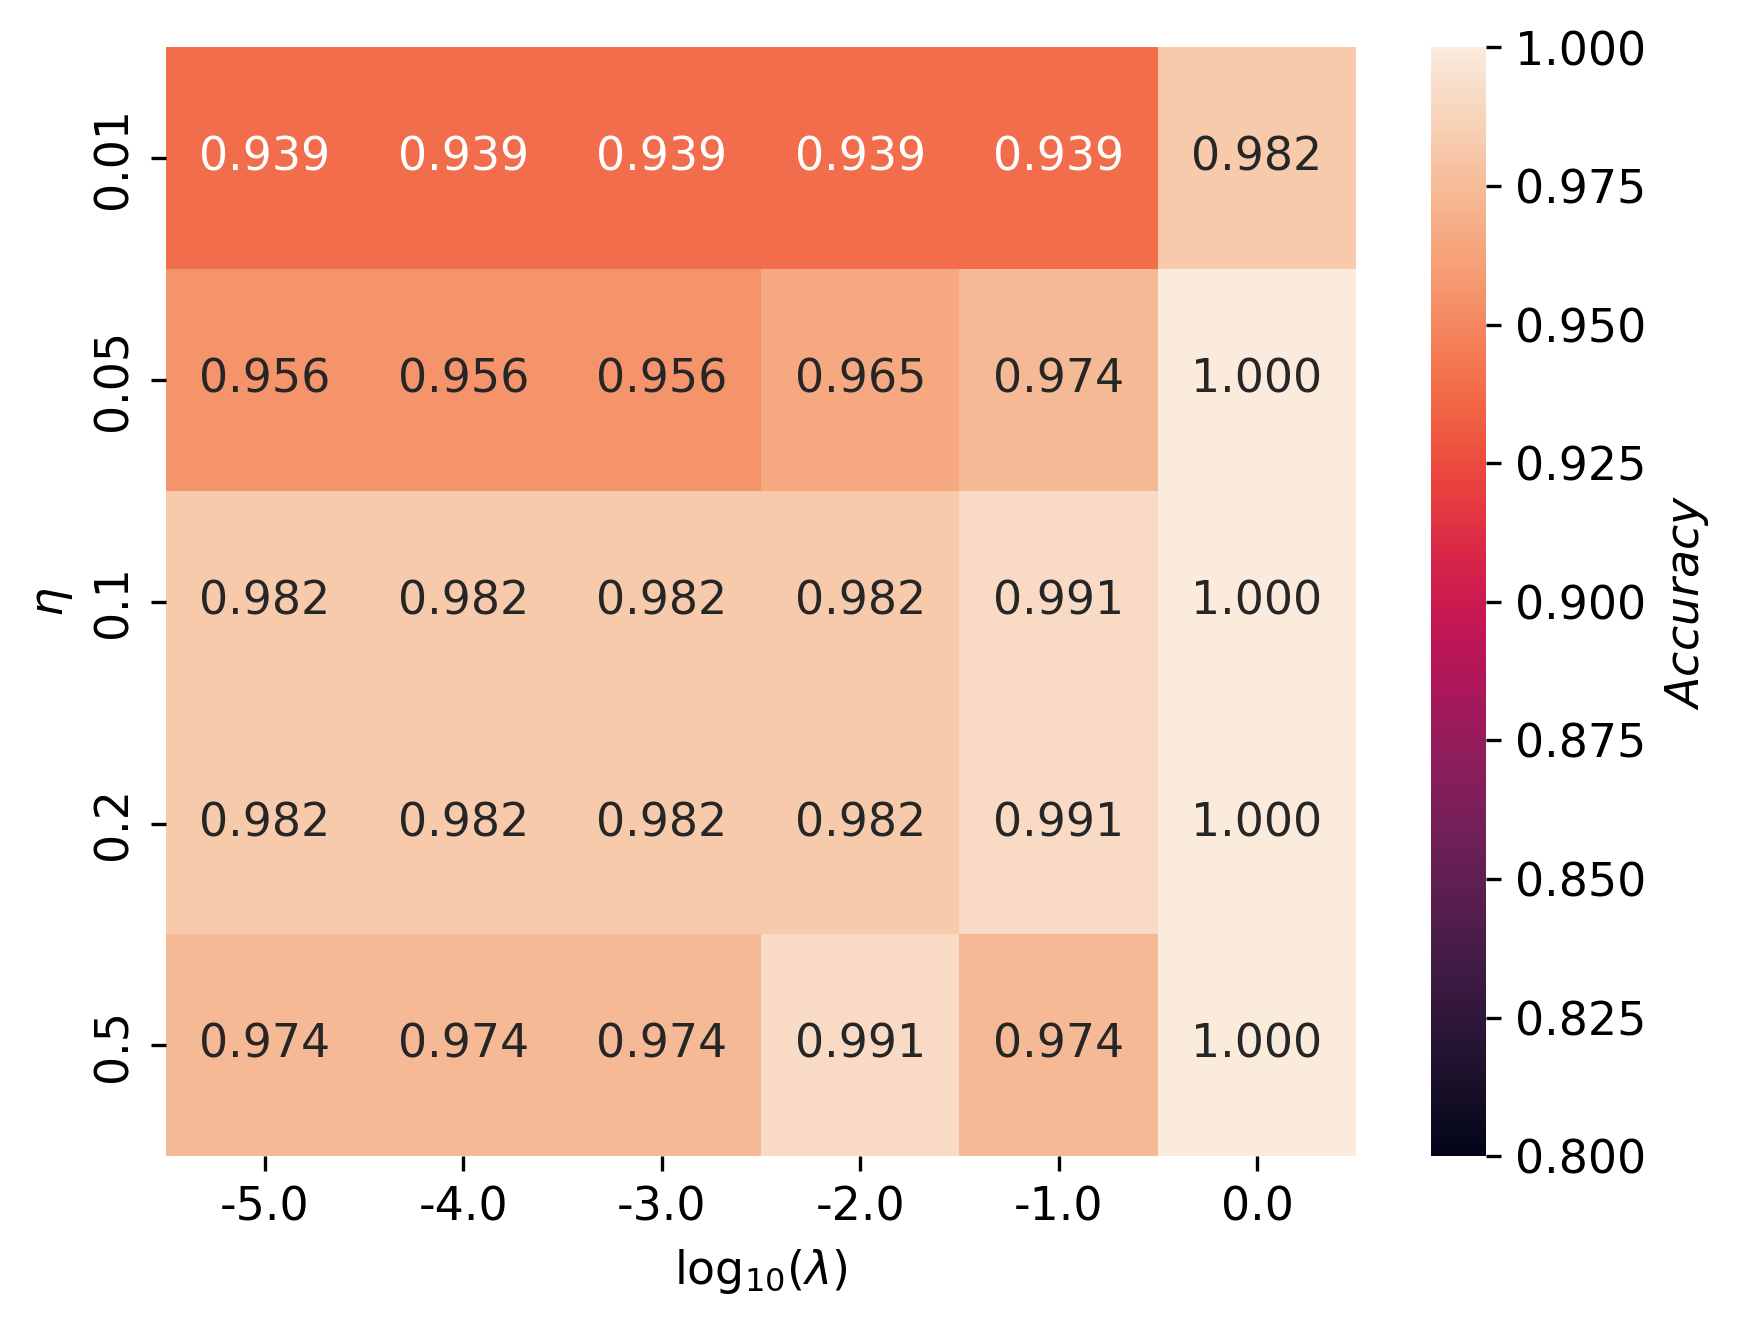
\includegraphics[width=\textwidth]{../figures/cancer_eta_lmb_best.png}
        \caption{Own neural network}
        \label{fig:}
    \end{subfigure}
    \begin{subfigure}{.5\textwidth}
        \centering
        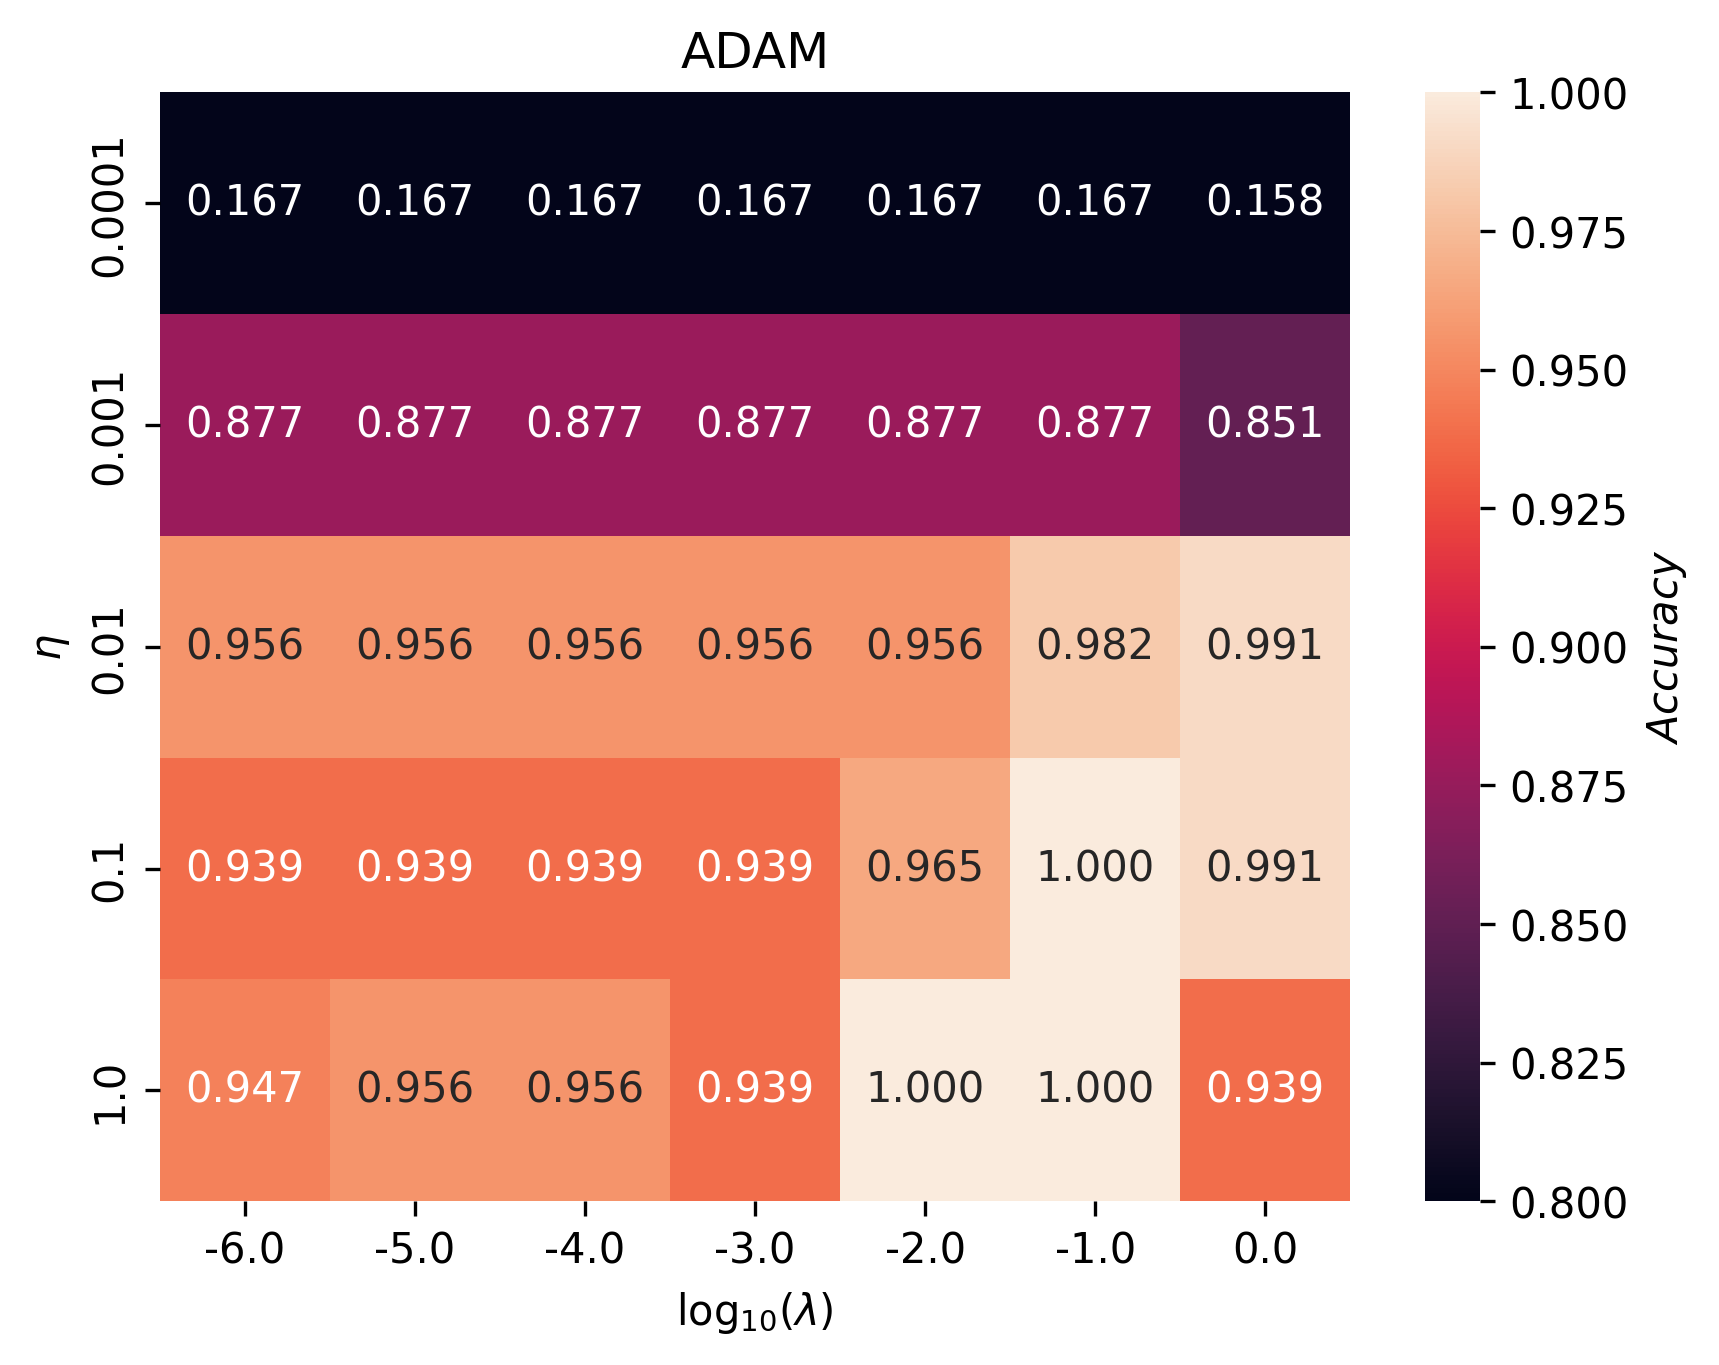
\includegraphics[width=\textwidth]{../figures/logreg_ADAM_best.png}
        \caption{Logistic regression using ADAM}
        \label{fig:}
    \end{subfigure}
    \caption{Accuracy of our own Neural Network for different choices of $\eta$, $\lambda$ and logistic regression using SGD and ADAM for a different train-test split than in figure \ref{fig:NN_cancer} and \ref{fig:logreg_comp}}
    \label{fig:cancer_best}
\end{figure}
We see in figure \ref{fig:cancer_best} that a different shuffle in the train-test split gives us accuracies up to 100\% for both logistic regression and our neural network.
\section{Discussion}
\subsection{Gradient descent}
When looking at figure \ref{fig:compare_GD_SGD} and \ref{fig:compare_GD_SGD_2} we saw that the SGD both performed better and converged faster than normal GD. This leaves us with SGD generally being the method of choice when performing gradient descent. Here it is still worth noticing that the $MSE$ for GD has been calculated as a minimum over all iterations and for SGD at the last iteration. We are therefore not left with a good comparison between the two methods for any given number of iteration, but rather a general indication of performance.
We also see that the different tuning methods have spikes in their $MSE$ at different iterations meaning that a direct comparison at one iteration would not give us any valuable information about the general performance of the methods. These spikes show us the importance of also choosing the right number of iterations or even stop the iterating process when the computed gradient reaches some minimal value $\epsilon$. This has not been done in both the gradient descent methods and the neural network which may have given us worse results from a never stopping oscillating behavior when reaching the global minimum.

When comparing the different tuning methods in table \ref{tab:OLS_compare} it is clear that no tuning has a great cost of performance. No tuning performs in almost all cases worse than all the other tuning functions with ADAM, RMSprop and AdaGrad taking turn in performing the best. This can be explained by how these methods perform their stepping process. They all change the stepping rate depending on the gradient which for ADAM and RMSprop get greatly reduced in regions with gradients of large magnitude. The same can be said about AdaGrad when using SGD. This gives the possibility to use larger learning rates and thereby make the algorithms converge faster towards the global minimum ignoring local minima. They also minimize oscillations around a global minimum from the reduction in the stepping process where the gradient is small.  These methods come with a minimal cost of computing time and can at the same time as seen greatly improve performance.

In table \ref{tab:OLS_compare} we saw that SGD with AdaGrad, RMSprop and ADAM performed better than OLS. Here it is worth noticing that we have not made any optimizations for OLS and used a design matrix of degree 6 when analyzing 4th degree data. In project 1 \cite{project1} we saw when analyzing OLS that we can have a great increase in $MSE$ from overfitting which may be the case here. Our results do therefore not tell us that SGD is generally better than OLS, but rather that it may outperform OLS when a wrong design matrix is chosen. In other words are our gradient descent methods less prone to overfitting.

When looking at our results from Ridge regression from table \ref{tab:ridge_compare_GD} and \ref{tab:ridge_compare_SGD} we see generally better performance than what we saw for OLS, but for AdaGrad we see worse performance. This is not what we would expect after introducing the L2-norm $\lambda$. This is a perfect example of what we discussed earlier. Since we for ridge regression compute the $MSE$ at the last iteration, the values can vary a lot depending on if we have a spike in $MSE$ or not at the last iteration where the $MSE$ is computed.


In all earlier analysis of our one dimensional function we have used a batch size of 16 giving us 5 minibatches. This choice is made based on a balance between computation time and performance, and as we saw in figure \ref{fig:compare_batch_size} this batch size generally converges fast and performs well. We see that larger batch sizes performs worse and that smaller batch sizes only equals small performance gains. We also saw that a batch size of 40 in most cases outperforms a batch size of 20. This can be explained by the shuffle algorithm of the input and target data for each minibatch. This shuffle has been made with a seed to be able to reproduce the results, but when the size of the minibatch varies, the shuffle will too. Because of this it is hard to gain anything more than an indication of what batch size gives the best performance to compute time ratio. A more statistical analysis using for example bootstrap could on the other hand given us information helping us choose the best possible batch size fitting our needs of performance and computation time.

\subsection{Franke function}
For the Franke function we saw in figure \ref{fig:franke_grid}, \ref{fig:franke_grid_2} and \ref{fig:franke_grid_3} together with table \ref{tab:franke_best} that our own neural network using sigmoid as activation function performed best. Here all the target data was scaled to the interval [0,1] for simplicity, which may not have been beneficial for ReLU and leaky ReLU. These methods would prefer to have standard scaled input data \cite{deeplearning} to avoid the weights of the neural network growing large. So even if we have performed a grid search finding the optimal parameters for ReLU and leaky ReLU, we have not used optimal input data and have in that way compromised their performance. An indication of this can be seen in table \ref{tab:franke_best} where the two ReLU functions have optimal learning rates of $\eta=0.02$ which is 10 times lower than sigmoid. Higher learning rates may have started seeing an exploding gradient followed by too fast-growing weights. To improve performance, methods such as batch normalization can be used. This method normalizes the data of each minibatch making it possible to use much higher learning rates both improving performance and allowing for up to 14 times fewer training steps \cite{batchnormalization}. This is left as a further improvement to be implemented in our neural network.

When comparing figure \ref{fig:franke_grid} for sigmoid to \ref{fig:franke_grid_2} for ReLU we saw that different learning rates have been used in the grid search. This is again because of exploding gradients and thereby overflow for the ReLU functions when using learning rates higher than 0.1. In total does our results not show that the sigmoid function is superior for a regression problem, but that it for a min-max scaling between 0 and 1 would outperform the ReLU activation functions. Another way to reduce the performance issues for ReLU could be to let the model run over more iterations which would in the gradient descent process allow for lower learning rates. This may also be beneficial when using sigmoid as activation function. But the performance gains of this will always have to be balanced to the cost of computation time.  An implementation of a scaling function such as ADAM, RMSprop or AdaGrad could also be of help. Adding momentum which in our case was set to 0 could also as seen for the one dimensional function \ref{tab:OLS_compare} greatly improve performance. These are all left as possible improvements for our neural network.

When comparing the two ReLU functions we notice that the leaky ReLU function performs worse. The leaky ReLU function removes a problem found using ReLU with neurons becoming inactive. This would indicate the leaky ReLU being the superior method. An explanation of the leaky ReLU performing worse in our case can also be connected to the scaling of our data. Another explanation may just be the initialization of our weights which in both cases are initialized using the same seed. Another seed may see the opposite results which is what we have seen for TensorFlow keras neural network which greatly varies in performance each time it runs. In order to properly understand the activation functions a statistical approach would be needed. We could then gain an expected value of our neural network for the different methods which would give us a way to differentiate the methods' performance.

\subsection{Cancer data}
In table \ref{tab:cancer_comp} we saw that both our logistic regression using gradient descent and our Neural network performed better than scikit learn's built in logistic regression functionality. Here it is worth noticing that we have used scikit's default settings which may not have been optimal. A direct performance comparison to our other methods where optimal parameters would therefor not be fair.

When initializing and splitting our data in train and test sets we performed a shuffle. The same shuffle were performed every time to be able to compare the methods and reproduce the data. What we saw when using other seeds for the shuffle was that the accuracy of the methods could greatly vary, and even giving accuracies of up to 100\% on test data as we saw in figure \ref{fig:cancer_best}. This means that the contents and order of the train and test data influences our results, indicating that a single prediction can not be taken as the expected performance of both our neural network and the logistic regression methods. A bootstrap analysis could be beneficial for understanding the methods' performance when we have limited data at hand, and is left as a possibility to better understand the performance of our methods. Furthermore, would such an analysis help us to accurately choose which method that is best for breast cancer data. As of now we can only say that both a neural network and logistic regression performs well, and that the only choosing factor that is left is computation time and simplicity of implementation. From this would the logistic regression using SGD and a tuning function such as ADAM be the method of choice.

When analyzing the cancer data, only the sigmoid activation was used from this function seeming to be the better choice for the other datasets.  This means that the output layer got numbers in the interval [0,1] and not only 0 and 1 which are the only possible outcomes. Even though the output data was given values of 0 or 1 after the neural network's predictions, an output activation function such as softmax already outputting 0 or 1 could help to improve performance. We could also combine softmax with the ReLU functions for activation of the hidden layers adding more possibilities to optimize the neural network depending on the problem.

\section{Conclusion}
We have looked at different gradient descent methods and seen that stochastic gradient descent together with a tuning function such as ADAM, RMSprop or AdaGrad generally performs best. In the case of a one-dimensional function this was especially true. AdaGrad reached a $MSE$ of 0.00774 while no tuning has a $MSE$ of 0.01158 when using SGD and a learning rate $\eta=0.1$. For logistic regression on cancer data we found that no tuning performed just as well as the other methods. We ended up using no tuning function in the stochastic gradient descent of our neural network which ends up being a possible further improvement, especially when using ReLU and leaky ReLU which showed poor performance on predicting the Franke function compared to sigmoid with $MSE$ of 0.041 and 0.042 and 0.039 respectively. Furthermore, a scaling in form of methods such as standard scaling or batch normalization are also possibilities for performance improvement of the neural network, which especially may help the ReLU functions in performing better. When it comes to the classification case of predicting breast cancer data we saw great performance for both our neural network and our logistic regression both outperforming scikit learn's built in logistic regression functionality. For both the classification and regression case, we need a further statistical analysis to accurately be able to compare the methods used. We are on the other hand left with indications of our neural network being better than both OLS and Ridge for regression, and logistic regression being the method of choice for a classification case as a result of its simple implementation and fast computation. When using gradient descent we also found that stochastic gradient descent paired with either AdaGrad, ADAM or RMSprop gave the best results.
\nocite{nielsen}
\nocite{Mehta_2019}
\nocite{hastie}
\printbibliography
\end{document}
